\documentclass[11pt]{article}

% --- Encoding / typography ---
\usepackage[utf8]{inputenc}
\usepackage[T1]{fontenc}
\usepackage{lmodern}
\usepackage{microtype}
\usepackage{setspace}
\usepackage{graphicx}
\usepackage{xurl}
\usepackage{url}
\usepackage{subcaption}
\usepackage{float}
\usepackage{placeins}
\def\UrlBreaks{\do\_}

\setstretch{1.05}

% --- Page layout ---
\usepackage[margin=1in]{geometry}

% --- Lists / tables (included even if the current text uses mostly prose) ---
\usepackage{booktabs}
\usepackage{longtable}
\usepackage{tabularx}
\usepackage{enumitem}

% --- Links ---
\usepackage[hidelinks]{hyperref}

% --- Section styling ---
\usepackage{titlesec}
\titleformat{\section}{\Large\bfseries}{\thesection}{0.75em}{}
\titlespacing*{\section}{0pt}{1.25em}{0.5em}

% --- Paragraph style ---
\setlength{\parindent}{0pt}
\setlength{\parskip}{0.55em}

\newcommand{\cvversion}{1.0.2} % TODO(me): update at release

\title{%
  \vspace*{-1cm}
  
\includegraphics[width=0.28\textwidth]{Figures/logo.png}\par
  \vspace{0.6cm}
  \textbf{Cellivista scRNA-seq Shiny App}\\Vignette and User Guide\\[0.3em]
  {\large Version \cvversion}
}
\author{}
\date{Generated \today }

\begin{document}

\maketitle

\begin{abstract}
This document describes the end-to-end workflow implemented in the Cellivista R/Shiny codebase: converting matrix-format single-cell data to Seurat RDS files, loading 10x Genomics HDF5 or Seurat RDS data, quality control, filtering, doublet removal, integration, clustering/visualization, marker discovery, annotation, gene-level feature plots, and a Visualization Options tab for UMAP palettes, marker heatmaps, and cluster composition plots. The vignette is written to be suitable as a methods supplement for publication, with clear inputs, outputs, and parameter definitions.
\end{abstract}
\newpage

\tableofcontents
\newpage

\section{Overview}
The application is a multi-tab Shiny interface that guides users through a typical Seurat-based single-cell RNA-seq analysis pipeline. Each tab corresponds to a logical stage in the analysis workflow, allowing users to interactively adjust settings through the interface and visualize results without writing any code.

\textbf{Key design features}
\begin{itemize}
  \item Accepts uploads up to 25 GB by default. To change the limit, set the environment variable \texttt{CELLIVISTA\_MAX\_UPLOAD\_GB} or the R option \texttt{cellivista.max\_upload\_gb} before starting the app.
  \item Accepts either raw 10x Genomics HDF5 files (\texttt{.h5}) or prebuilt Seurat objects (\texttt{.rds}).
  \item Includes a matrix-to-RDS conversion sub-tab for users who have separate matrix, cell/barcode, and gene/feature files.
  \item {\raggedright Uses helper functions for the computational steps, including \texttt{convert\_matrix\_to\_rds()}, \texttt{read\_h5\_to\_seurat()}, \texttt{run\_qc\_metrics()}, \texttt{post\_qc\_filtering\_and\_plots()}, \texttt{remove\_doublets()}, \texttt{integrate\_seurat\_samples()}, \texttt{run\_downstream\_analysis()}, \texttt{run\_clusterwise\_dgea()}, \texttt{annotate\_clusters()}, \texttt{plot\_genes\_feature()}, \texttt{plot\_umap\_palette()}, \texttt{plot\_marker\_heatmap()}, and \texttt{plot\_cluster\_composition()}.\par}
  \item Also provides \texttt{run\_pairwise\_dgea()}, which compares two groups with \texttt{FindMarkers()}. It is used from R only; the app has no tab for it.
  \item Includes a \textbf{Visualization Options} tab for recoloring the UMAP, drawing a marker heatmap, and plotting cluster composition per sample (Section~\ref{sec:viz}).
  \item Provides plot previews, plot download buttons, and intermediate Seurat object downloads at key workflow stages.
 \item Includes a floating help widget that allows users to download both this vignette and the example dataset (Figure~\ref{fig:help_widget}).

\begin{figure}[h]
\centering
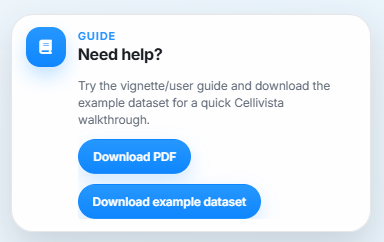
\includegraphics[width=0.5\textwidth]{Figures/help_widget.png}
\caption{Floating help widget in Cellivista providing direct access to the vignette and example dataset downloads.}
\label{fig:help_widget}
\end{figure}
  \item Example data and source code are also available from the Cellivista GitHub repository: \url{https://github.com/asinha639/cellivista}.
\end{itemize}

\subsection*{Sessions and downloads}
Cellivista keeps results per browser session. Plots, tables, and Seurat objects are written to a temporary folder for your session, and that folder is deleted when the session ends. Closing or refreshing the browser tab ends the session, so download anything you want to keep first. When the app runs on a shared server, each user who opens it gets a separate session with its own data and results.

\section{Software requirements}
\textbf{Core R packages}
\begin{itemize}
  \item \texttt{shiny}: Web application framework.
  \item \texttt{Seurat}, \texttt{SeuratObject}: Single-cell analysis framework.
  \item \texttt{Matrix}: Reading sparse matrix files during matrix-to-RDS conversion.
  \item \texttt{ggplot2}, \texttt{dplyr}: Plotting and data manipulation.
  \item \texttt{viridisLite}: The viridis palette in the Visualization Options tab.
  \item \texttt{withr}: Sets a temporary random seed when the marker heatmap samples cells, then restores the previous state.
  \item \texttt{base64enc}: Encoding saved plots for inline display in the Shiny interface.
  \item \texttt{patchwork}, \texttt{purrr}, \texttt{readr}: Plot composition, list/data utilities, and CSV input/output.
  \item \texttt{future}: Memory configuration and support for integration steps.
\end{itemize}

\textbf{Other packages}
\begin{itemize}
  \item \texttt{DoubletFinder}: Doublet detection. It is not on CRAN. Install it from GitHub with \texttt{remotes::install\_github("chris-mcginnis-ucsf/DoubletFinder")}.
  \item \texttt{hdf5r}: Needed only to read 10x Genomics \texttt{.h5} files.
  \item \texttt{svglite}: Optional. Needed only to export plots as \texttt{.svg}.
\end{itemize}

Notes

\begin{itemize}[leftmargin=*,nosep]
\item The code assumes a functioning C/C++ toolchain when compiling some dependencies (typical for Seurat/DoubletFinder).
\item For large datasets, memory requirements can be substantial; consider running the app on a machine with sufficient RAM.
\end{itemize}

\section{Step 1 -- Upload data}

\textbf{Purpose.}
This step allows users to either load an existing single-cell dataset into Cellivista or convert matrix-format files into a Seurat \texttt{.rds} object for later use.

The \textbf{Upload Data} tab contains two sub-tabs:
\begin{itemize}
  \item \textbf{Load Data}
  \item \textbf{Convert Matrix to RDS}
\end{itemize}

\subsection*{Load Data}

\textbf{What to do.}
Use this sub-tab to upload either a raw 10x Genomics HDF5 file (\texttt{.h5}) or a prebuilt Seurat object saved as an \texttt{.rds} file. The \texttt{.h5} option is intended for raw 10x-compatible count matrices, while the \texttt{.rds} option is intended for users who already have a valid Seurat object.

\textbf{What Cellivista does.}
\begin{itemize}
  \item Reads raw 10x Genomics \texttt{.h5} files and converts them into a Seurat object.
  \item Reads uploaded \texttt{.rds} files and verifies that they contain a valid Seurat object.
  \item Adds or normalizes the \texttt{SampleLabel} metadata field when needed.
  \item Calculates basic summary information for each cell, including detected features and total RNA counts.
  \item If multiple samples are present, preserves sample identity for later comparison, integration, and visualization.
\end{itemize}

\textbf{Key options explained.}
\begin{itemize}
  \item \textbf{Input type:} Selects whether the uploaded file is a raw 10x \texttt{.h5} file or a Seurat \texttt{.rds} object.
  \item \textbf{Sample label map:} Optional relabeling of sample IDs parsed from cell barcodes, using a format such as \texttt{Sample1=Control, Sample2=Treatment}.
  \item \textbf{Project name:} Project name assigned to the Seurat object when loading raw \texttt{.h5} data.
\end{itemize}

\textbf{Output.}
After this step, the dataset is loaded as a Seurat object and is ready for quality control.

\subsection*{Convert Matrix to RDS}

\textbf{Purpose.}
This sub-tab is provided for datasets distributed as separate matrix, cell/barcode, and gene/feature files rather than as a single \texttt{.h5} or \texttt{.rds} file. It converts those files into a Seurat \texttt{.rds} object that can then be uploaded through the \textbf{Load Data} sub-tab.

\textbf{What to do.}
Upload the matrix file, cell/barcode file, and gene/feature file. The matrix file is typically in Matrix Market format, such as \texttt{.mtx} or \texttt{.mtx.gz}. The cell and gene files may be plain-text, tab-delimited, comma-delimited, or compressed files depending on the source dataset.

\textbf{Important note about matrix-format datasets.}
Matrix, cell/barcode, and gene/feature files are not always standardized across public datasets. In particular, cell and gene files often have different column structures or column names depending on the data source. Cellivista provides suggested options for assigning gene names and sample labels, but these should be checked carefully before proceeding. In many cases, users must manually inspect the cell and gene files to confirm which column contains the correct barcode, gene symbol, gene ID, or sample label information.

\textbf{What Cellivista does.}
\begin{itemize}
  \item Reads the sparse matrix file.
  \item Reads the uploaded cell/barcode and gene/feature files.
  \item Assigns cell barcodes and gene names to the matrix.
  \item Creates a Seurat object using the selected minimum cell and feature thresholds.
  \item Adds a \texttt{SampleLabel} metadata field using the selected sample-label option.
  \item Saves the converted object as a downloadable Seurat \texttt{.rds} file.
\end{itemize}

\textbf{Key options explained.}
\begin{itemize}
  \item \textbf{Project name:} Project name assigned to the converted Seurat object.
  \item \textbf{Minimum cells per gene:} Genes detected in fewer than this number of cells are excluded.
  \item \textbf{Minimum features per cell:} Cells with fewer detected genes than this value are removed.
  \item \textbf{Sample label option:} Determines how \texttt{SampleLabel} metadata is created. Depending on the dataset, labels may come from barcode suffixes, a single user-provided sample label, or a column in the uploaded cell/barcode file.
  \item \textbf{Sample label column:} Used only when sample labels are stored in a specific column of the cell/barcode file. Users should manually verify the correct column before conversion.
\end{itemize}

\textbf{Output.}
This sub-tab produces a downloadable Seurat \texttt{.rds} file. After downloading it, users can return to the \textbf{Load Data} sub-tab, select \texttt{Seurat .rds object}, and upload the converted file to begin the standard Cellivista workflow.

\textbf{Example data.}
The example dataset used in this vignette can be downloaded from the floating help widget in the app. It is also available from the Cellivista GitHub repository: \url{https://github.com/asinha639/cellivista}.

\section{Step 2 -- Run quality control (QC)}

\textbf{Purpose.}  
This step evaluates the overall quality of your single-cell dataset and helps identify low-quality or damaged cells before downstream analysis.

\textbf{What to do.}  
Run the quality control step to visualize key metrics that describe each cell, such as the number of detected genes, total RNA content, and the fraction of mitochondrial transcripts.

\textbf{What Cellivista does.}
\begin{itemize}[leftmargin=*,nosep]
\item Calculates quality control metrics for every cell in the dataset.
\item Identifies mitochondrial genes and estimates the proportion of mitochondrial RNA, which is a common indicator of cell stress or degradation.
\item Generates clear visual summaries that allow users to assess data quality at a glance.
\end{itemize}

\textbf{How to interpret the plots.}
\begin{itemize}[leftmargin=*,nosep]
\item \textbf{Violin plots} show the distribution of quality metrics across all cells, helping identify unusually low- or high-quality populations.
\item \textbf{Scatter plots} highlight relationships between metrics (e.g., RNA content vs.\ mitochondrial percentage) and make outlier cells easier to detect.
\item If multiple samples are present, plots can be viewed separately for each sample to assess consistency.
\end{itemize}

\textbf{Key options explained.}
\begin{itemize}[leftmargin=*,nosep]
\item \textbf{Mitochondrial gene pattern:} Defines how mitochondrial genes are recognized. The default works for human data; an alternative is provided for mouse datasets.
\item \textbf{Metadata column to split violin plots:} The metadata column used to split the QC violin plots, so samples can be compared side by side. The default is \texttt{SampleLabel}.
\item \textbf{Y-limit for percent.mt plot:} Lower and upper y-axis bounds for the mitochondrial percentage plot. The default range is 0 to 80.
\end{itemize}

\textbf{Output.}  
This step produces quality control plots that can be reviewed and downloaded. The calculated QC metrics are stored internally and will be used in the next step to filter out low-quality cells.

\begin{figure}[htbp]
\centering
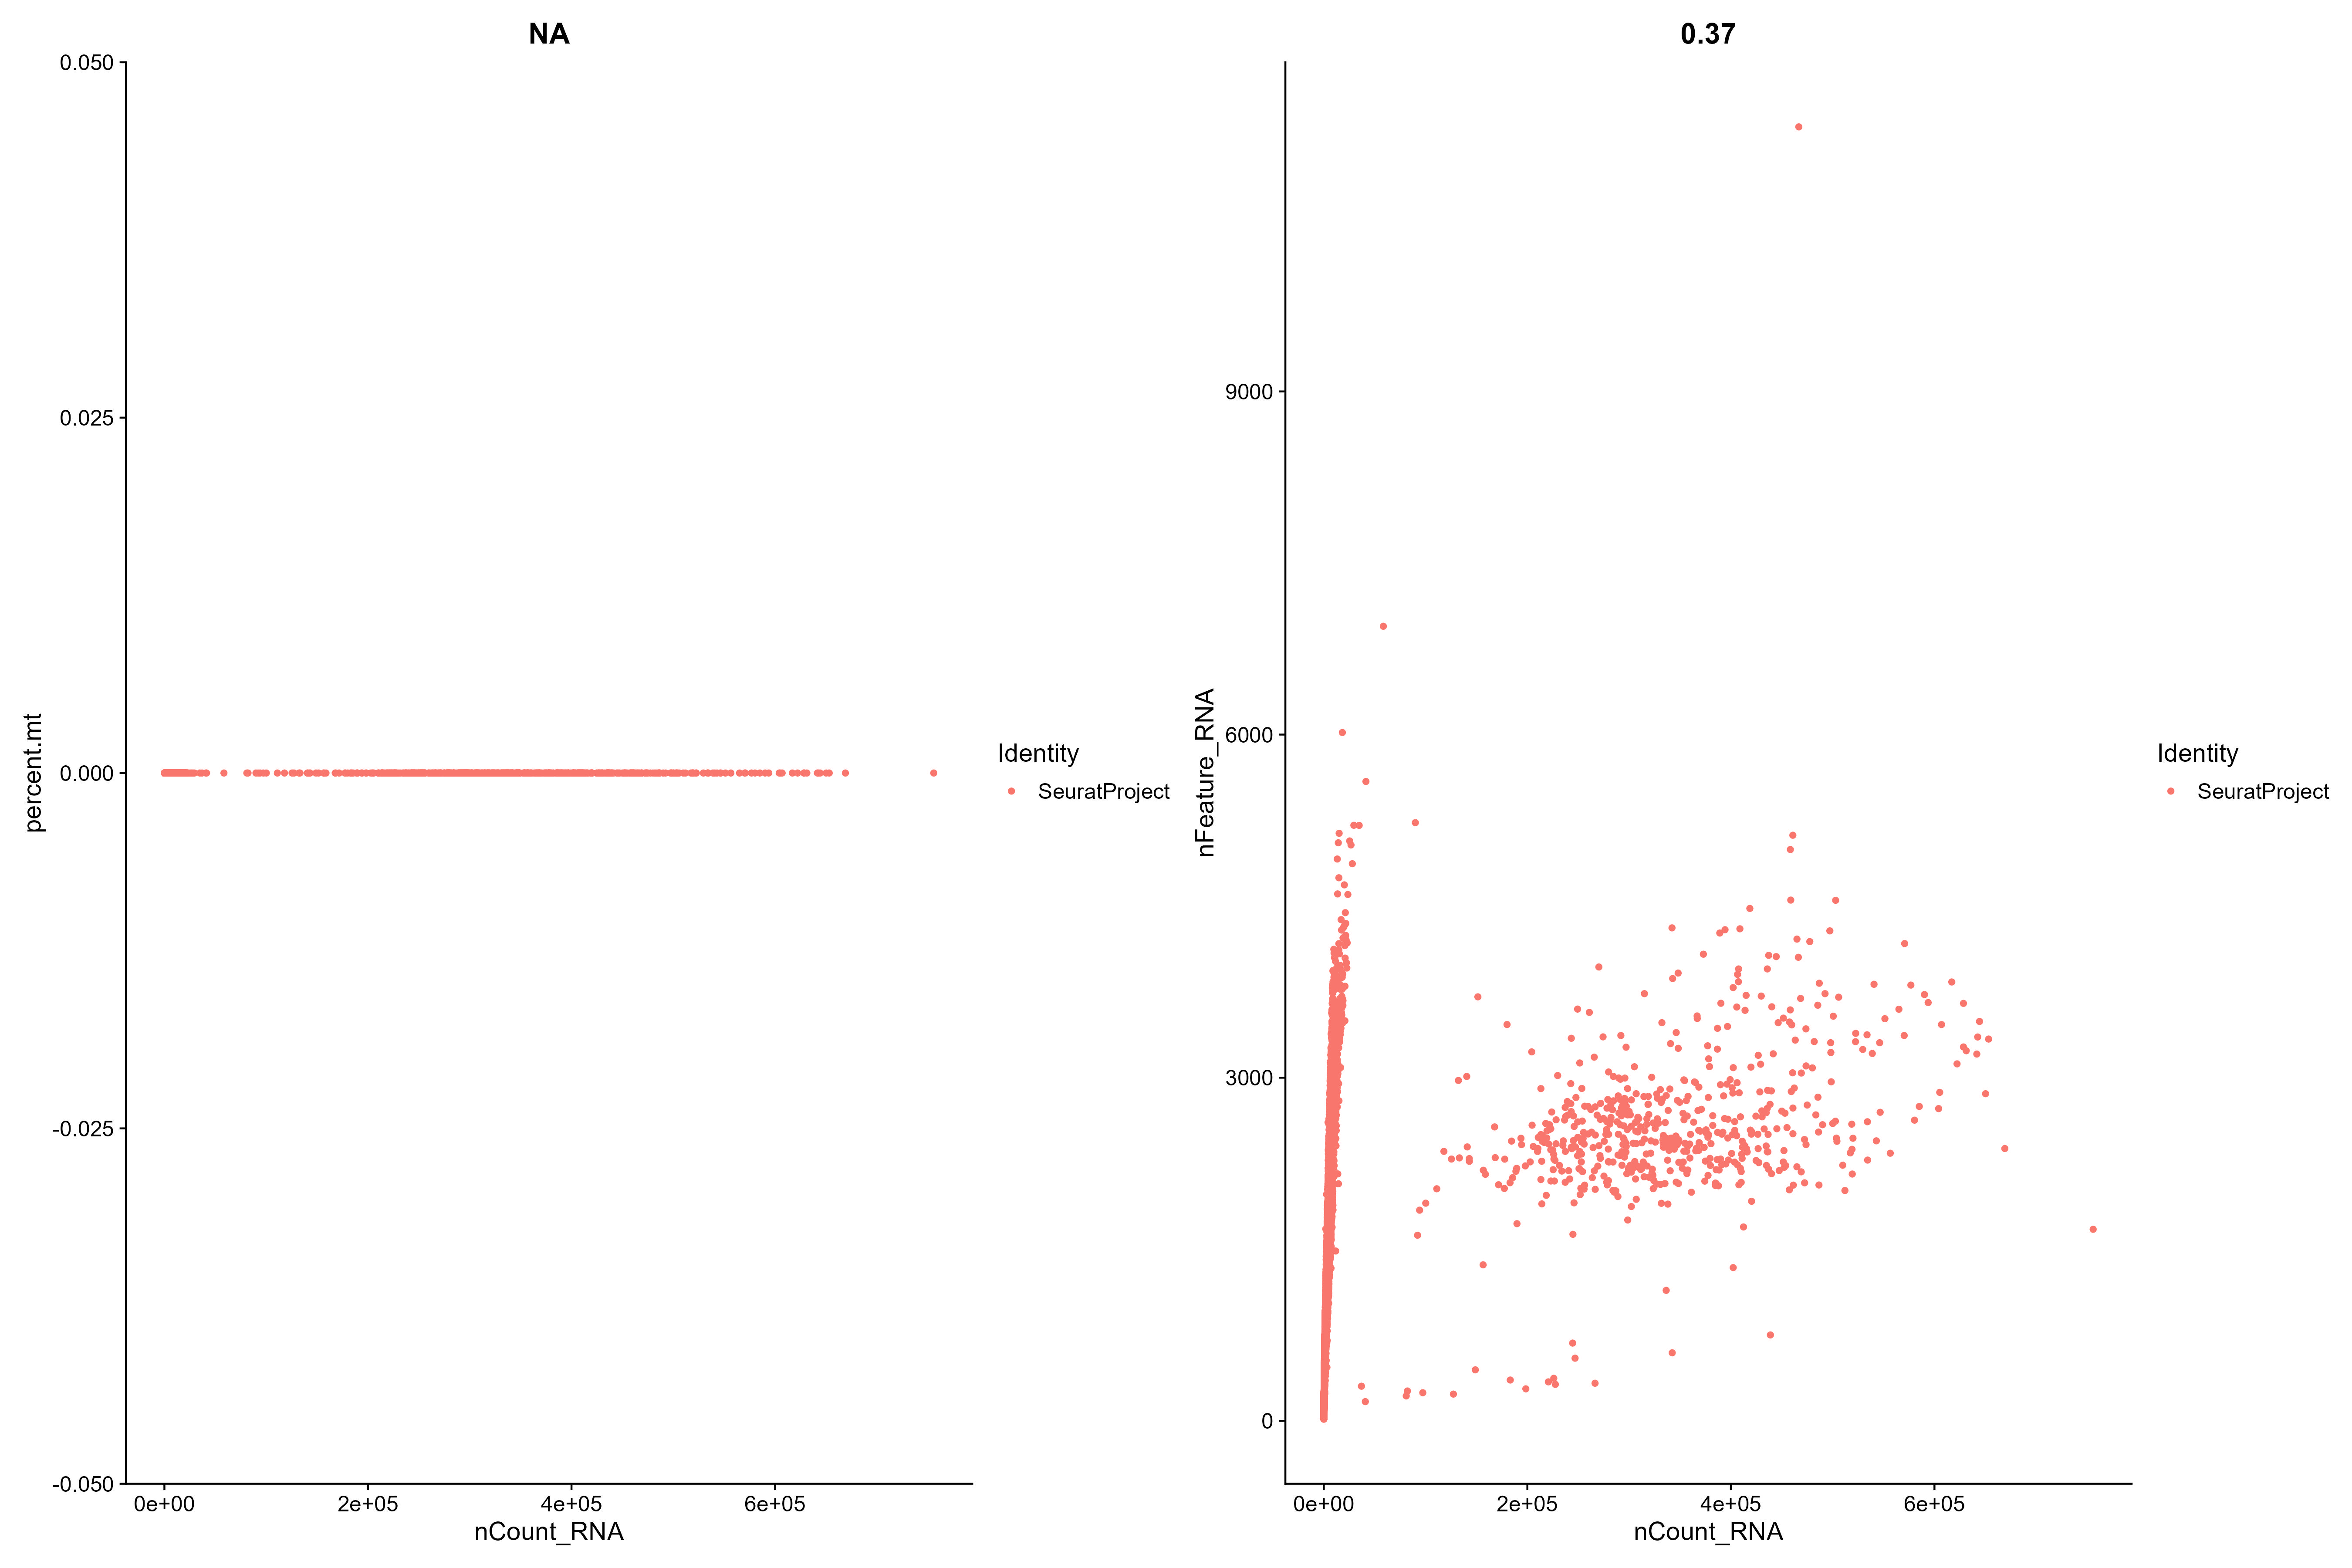
\includegraphics[width=0.32\textwidth]{Figures/pre_qc_FeatureScatterplot.jpg}
\hfill
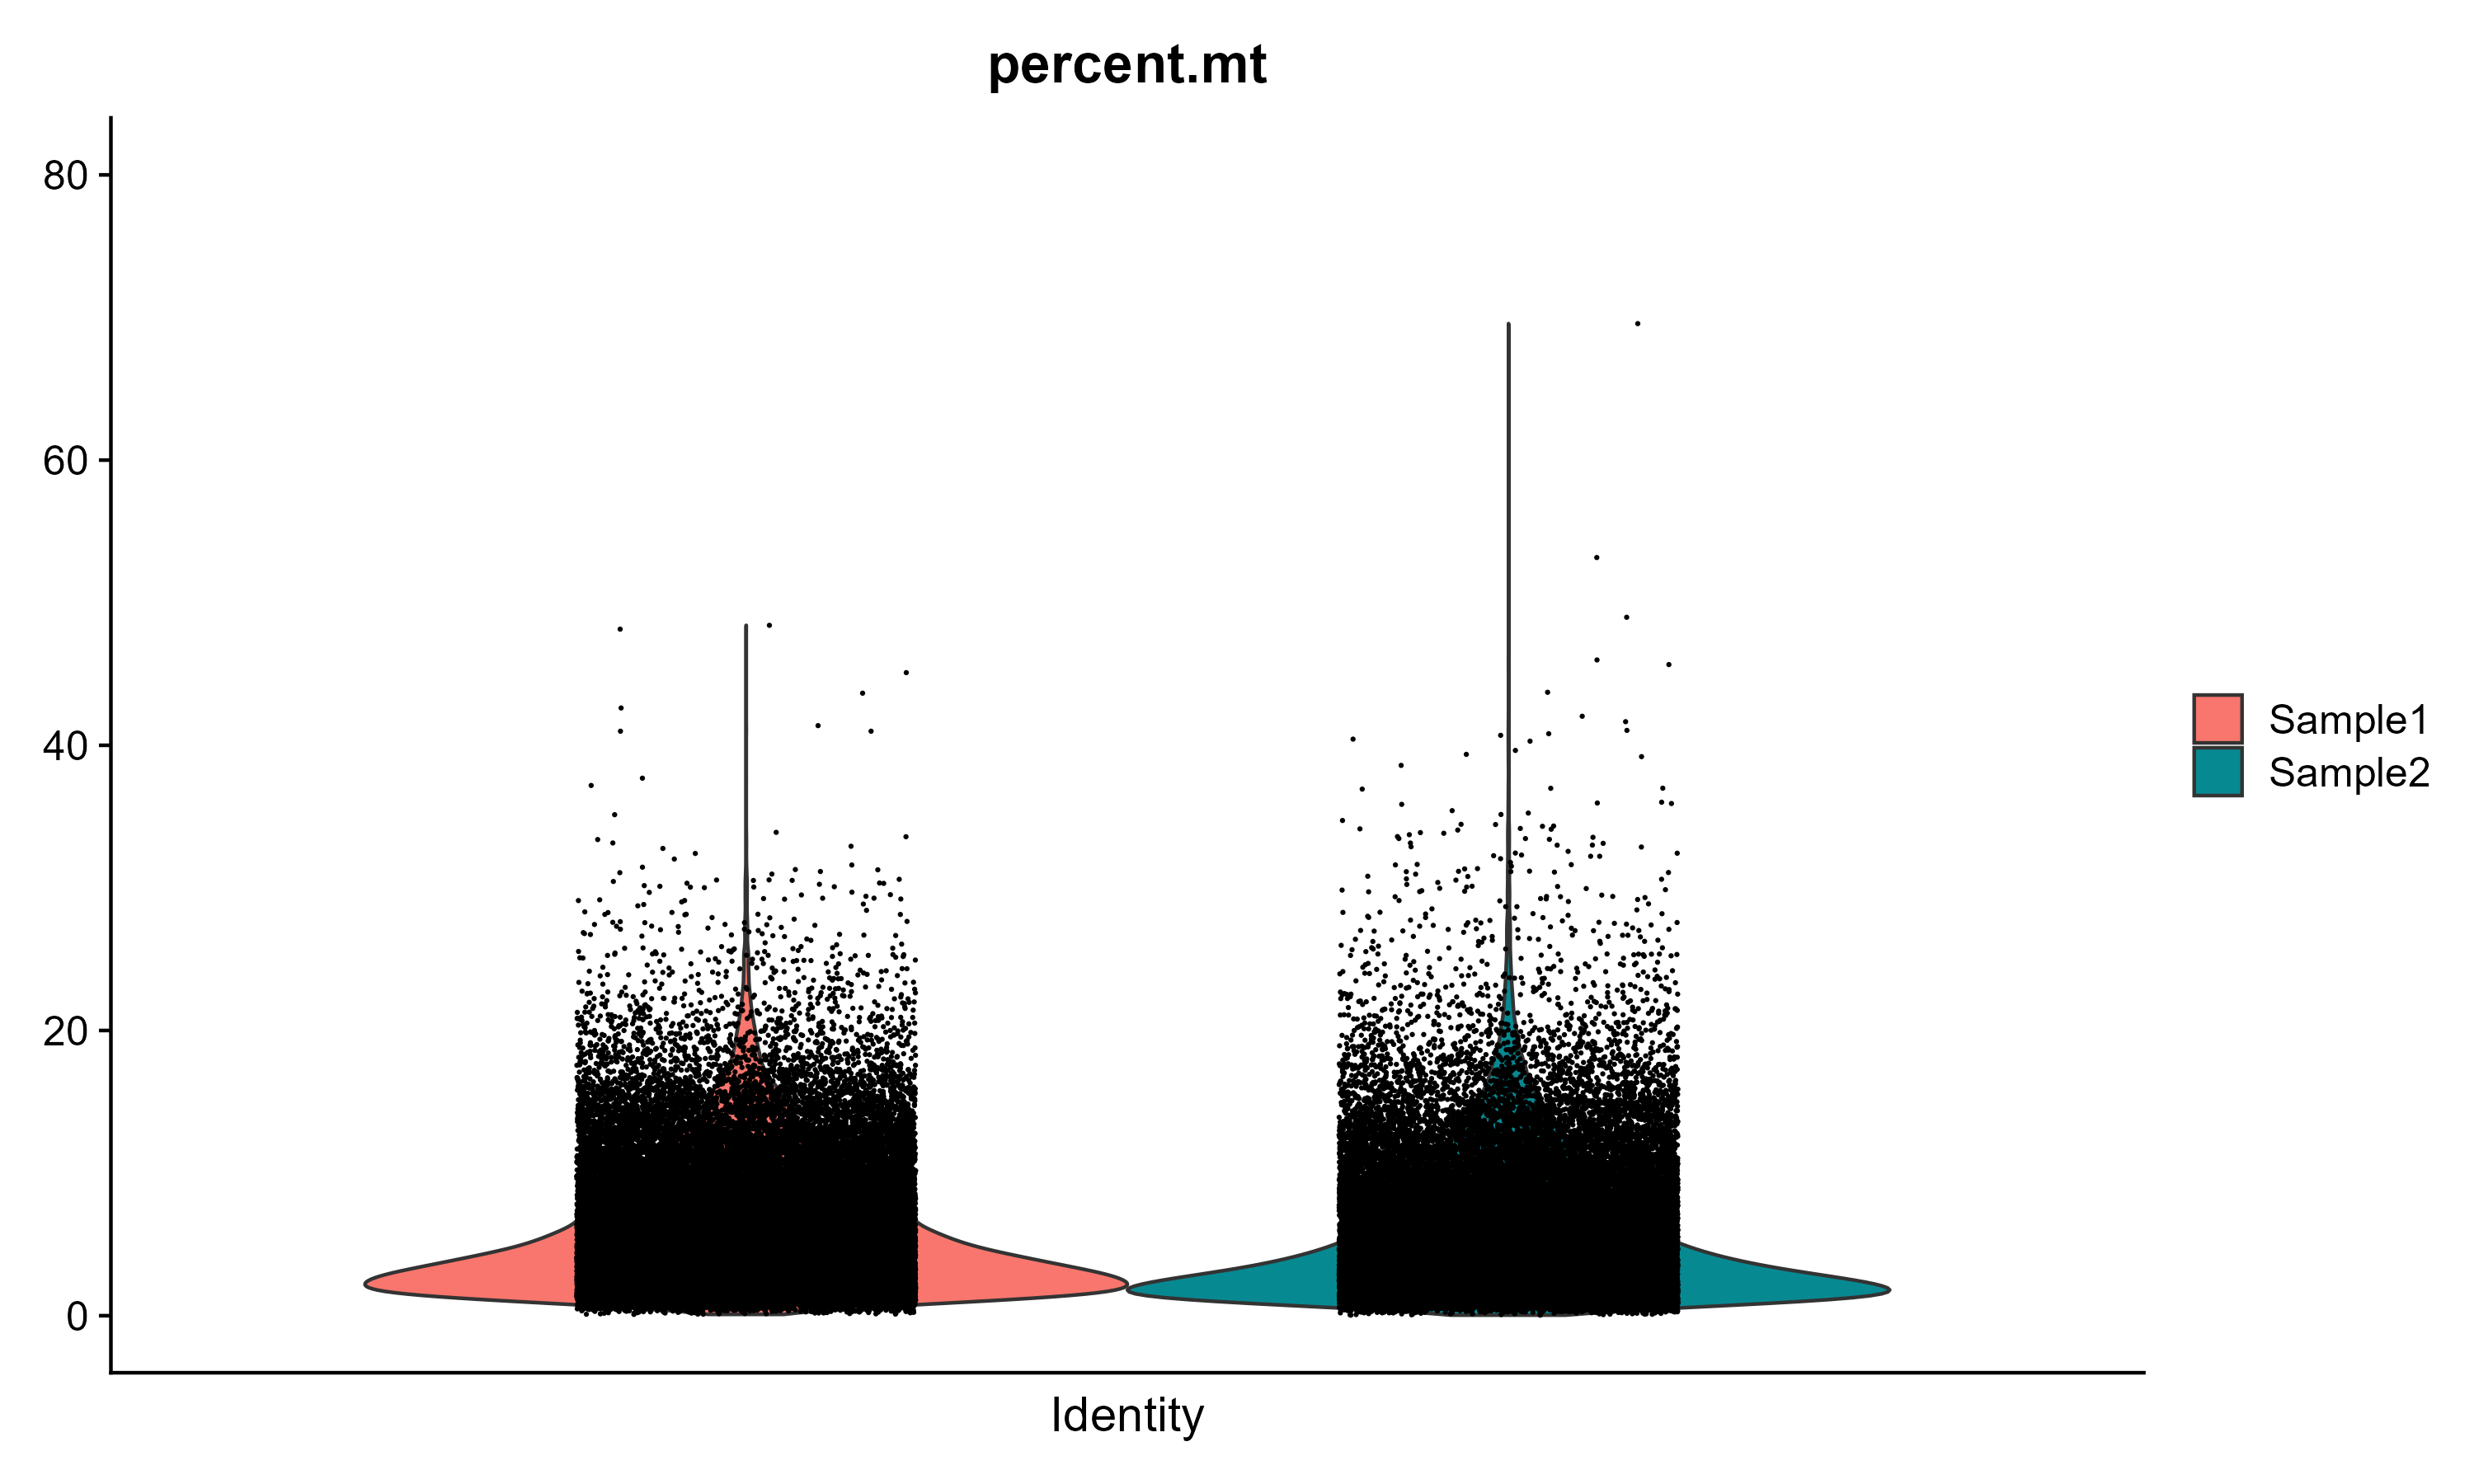
\includegraphics[width=0.32\textwidth]{Figures/pre_qc_percent.mt.png}
\hfill
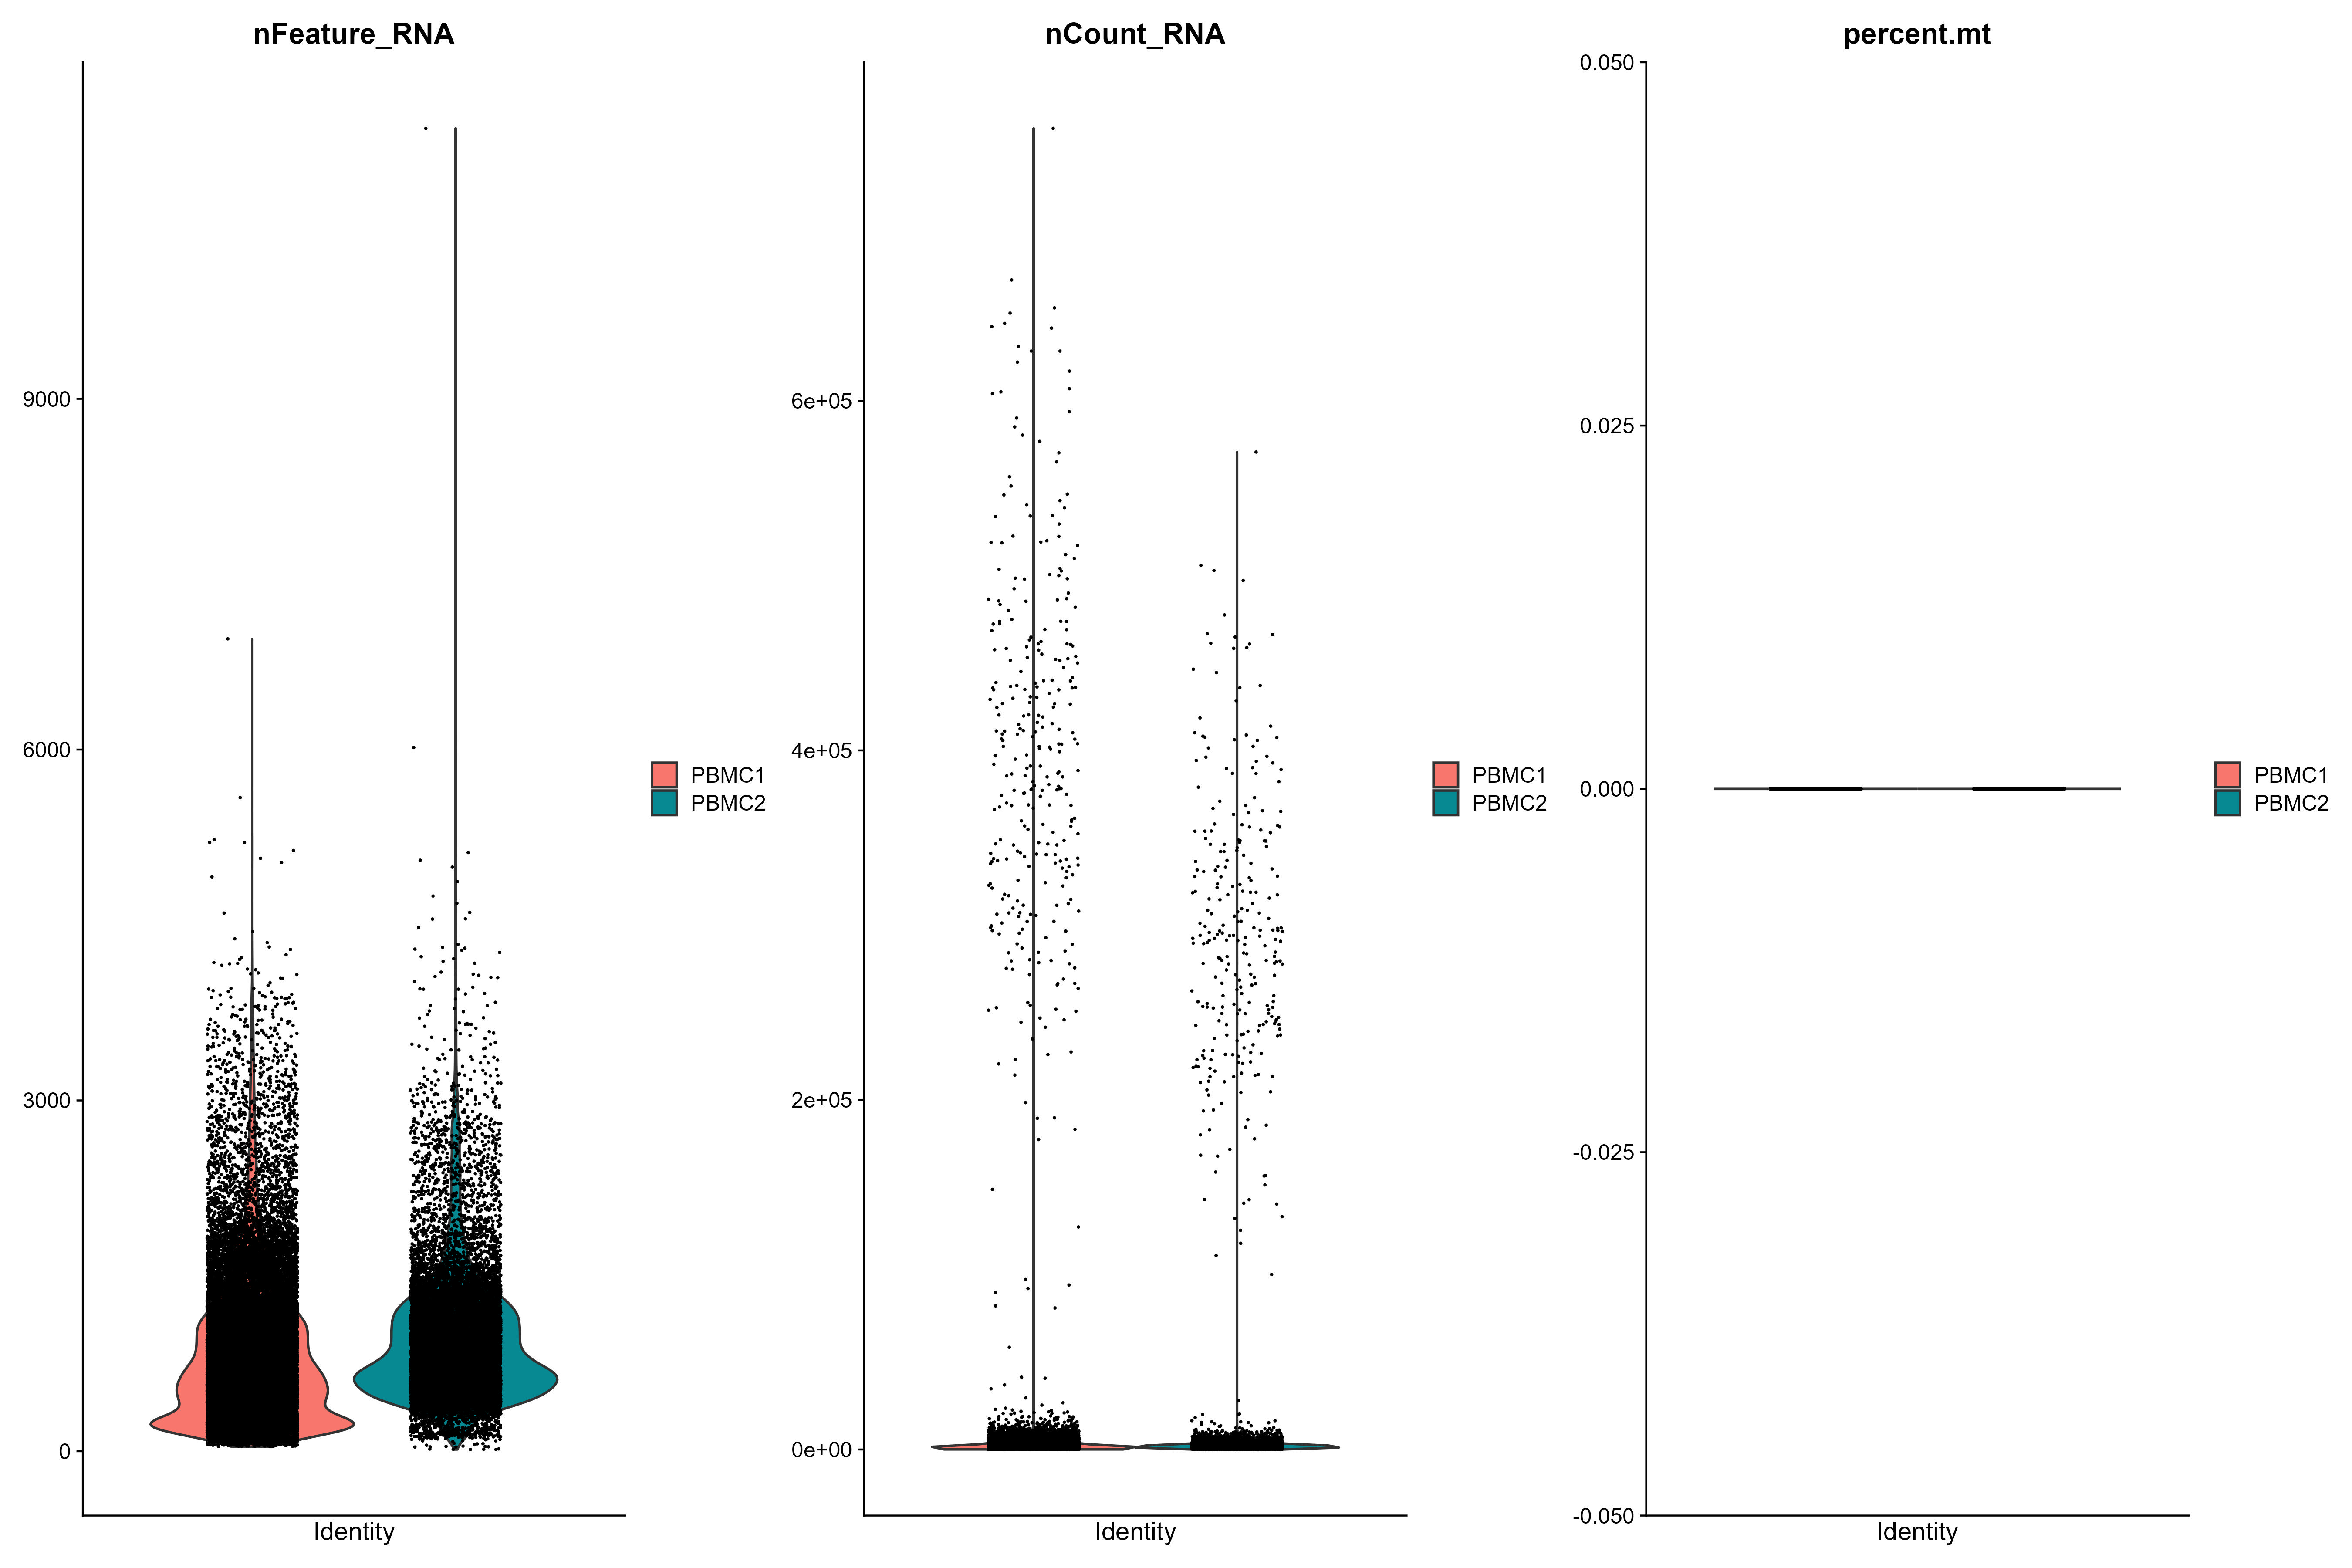
\includegraphics[width=0.32\textwidth]{Figures/pre_qc_violin.jpg}

\caption{Quality control visualizations generated during the QC step.
Left: relationship between total RNA counts and detected genes per cell.
Middle: distribution of mitochondrial transcript percentages.
Right: violin plots summarizing key QC metrics across all cells.}
\label{fig:qc_plots}
\end{figure}

\section{Step 3 -- Post-quality control filtering}

\textbf{Purpose.}  
This step removes low-quality cells and technical outliers identified during quality control, resulting in a cleaner and more reliable dataset for downstream analysis.

\textbf{What to do.}  
Based on the QC plots from the previous step, adjust filtering thresholds to exclude cells with unusually low or high gene detection, or high mitochondrial content. These thresholds can be refined iteratively to balance data quality and cell retention.

\textbf{What Cellivista does.}
\begin{itemize}[leftmargin=*,nosep]
\item Filters out cells that fall outside the selected quality thresholds.
\item Recalculates summary statistics after filtering to reflect the cleaned dataset.
\end{itemize}

\textbf{How to interpret the plots.}
\begin{itemize}[leftmargin=*,nosep]
\item \textbf{Density plots} show the distribution of total RNA counts per cell (\texttt{nCount\_RNA}) for each sample after filtering and help confirm that low-quality populations have been removed.
\item \textbf{Violin plots} summarize the remaining cells and allow comparison with pre-filtering distributions.
\end{itemize}

\textbf{Key options explained.}
\begin{itemize}[leftmargin=*,nosep]
\item \textbf{Minimum and maximum features per cell:} Removes cells with unusually low or high numbers of detected genes. The defaults are 200 and 7500.
\item \textbf{Maximum percent mitochondrial:} Filters cells with high mitochondrial RNA, often associated with cell stress or degradation. The default is 25.
\item \textbf{Split plots by:} The metadata column used to split the post-filtering plots. The default is \texttt{SampleLabel}.
\end{itemize}

\textbf{Output.}  
After filtering, the dataset contains only high-quality cells suitable for downstream analyses such as clustering and differential expression. Updated QC plots are generated and can be downloaded for record keeping or publication, and the filtered Seurat object can be downloaded as an \texttt{.rds} file.

\begin{figure}[H]
\centering
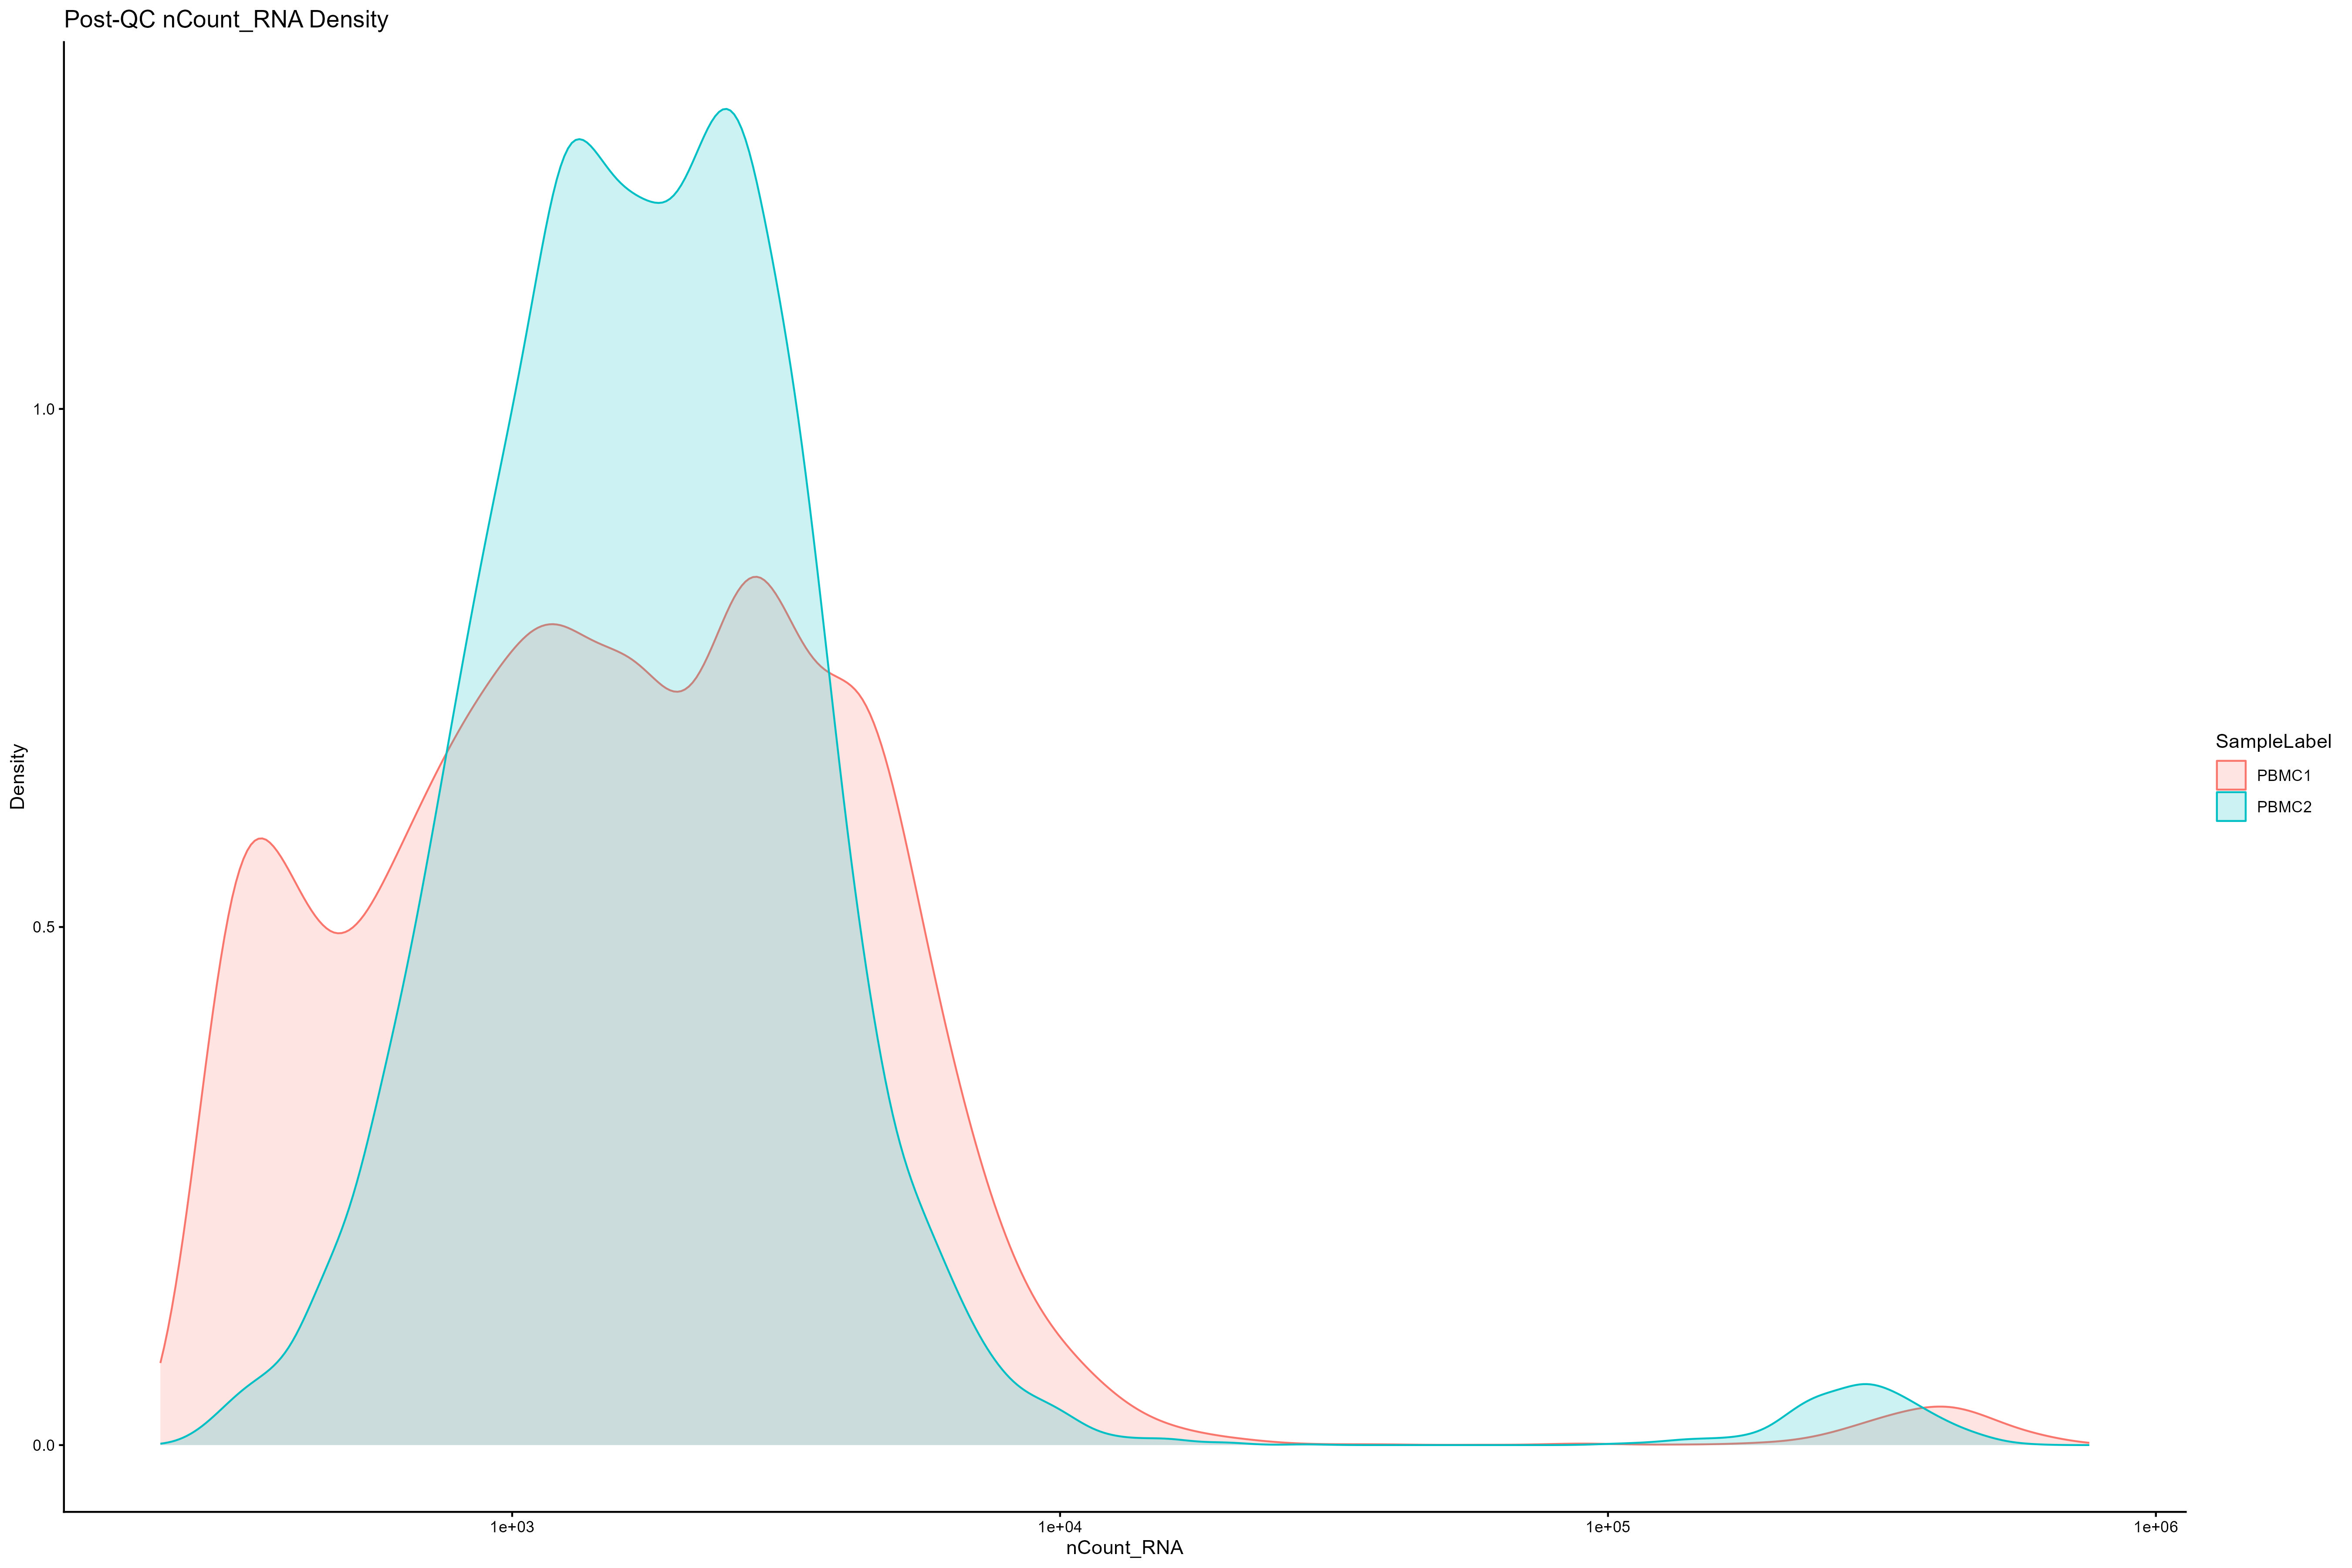
\includegraphics[width=0.48\textwidth]{Figures/post_qc_densityplot.jpg}
\hfill
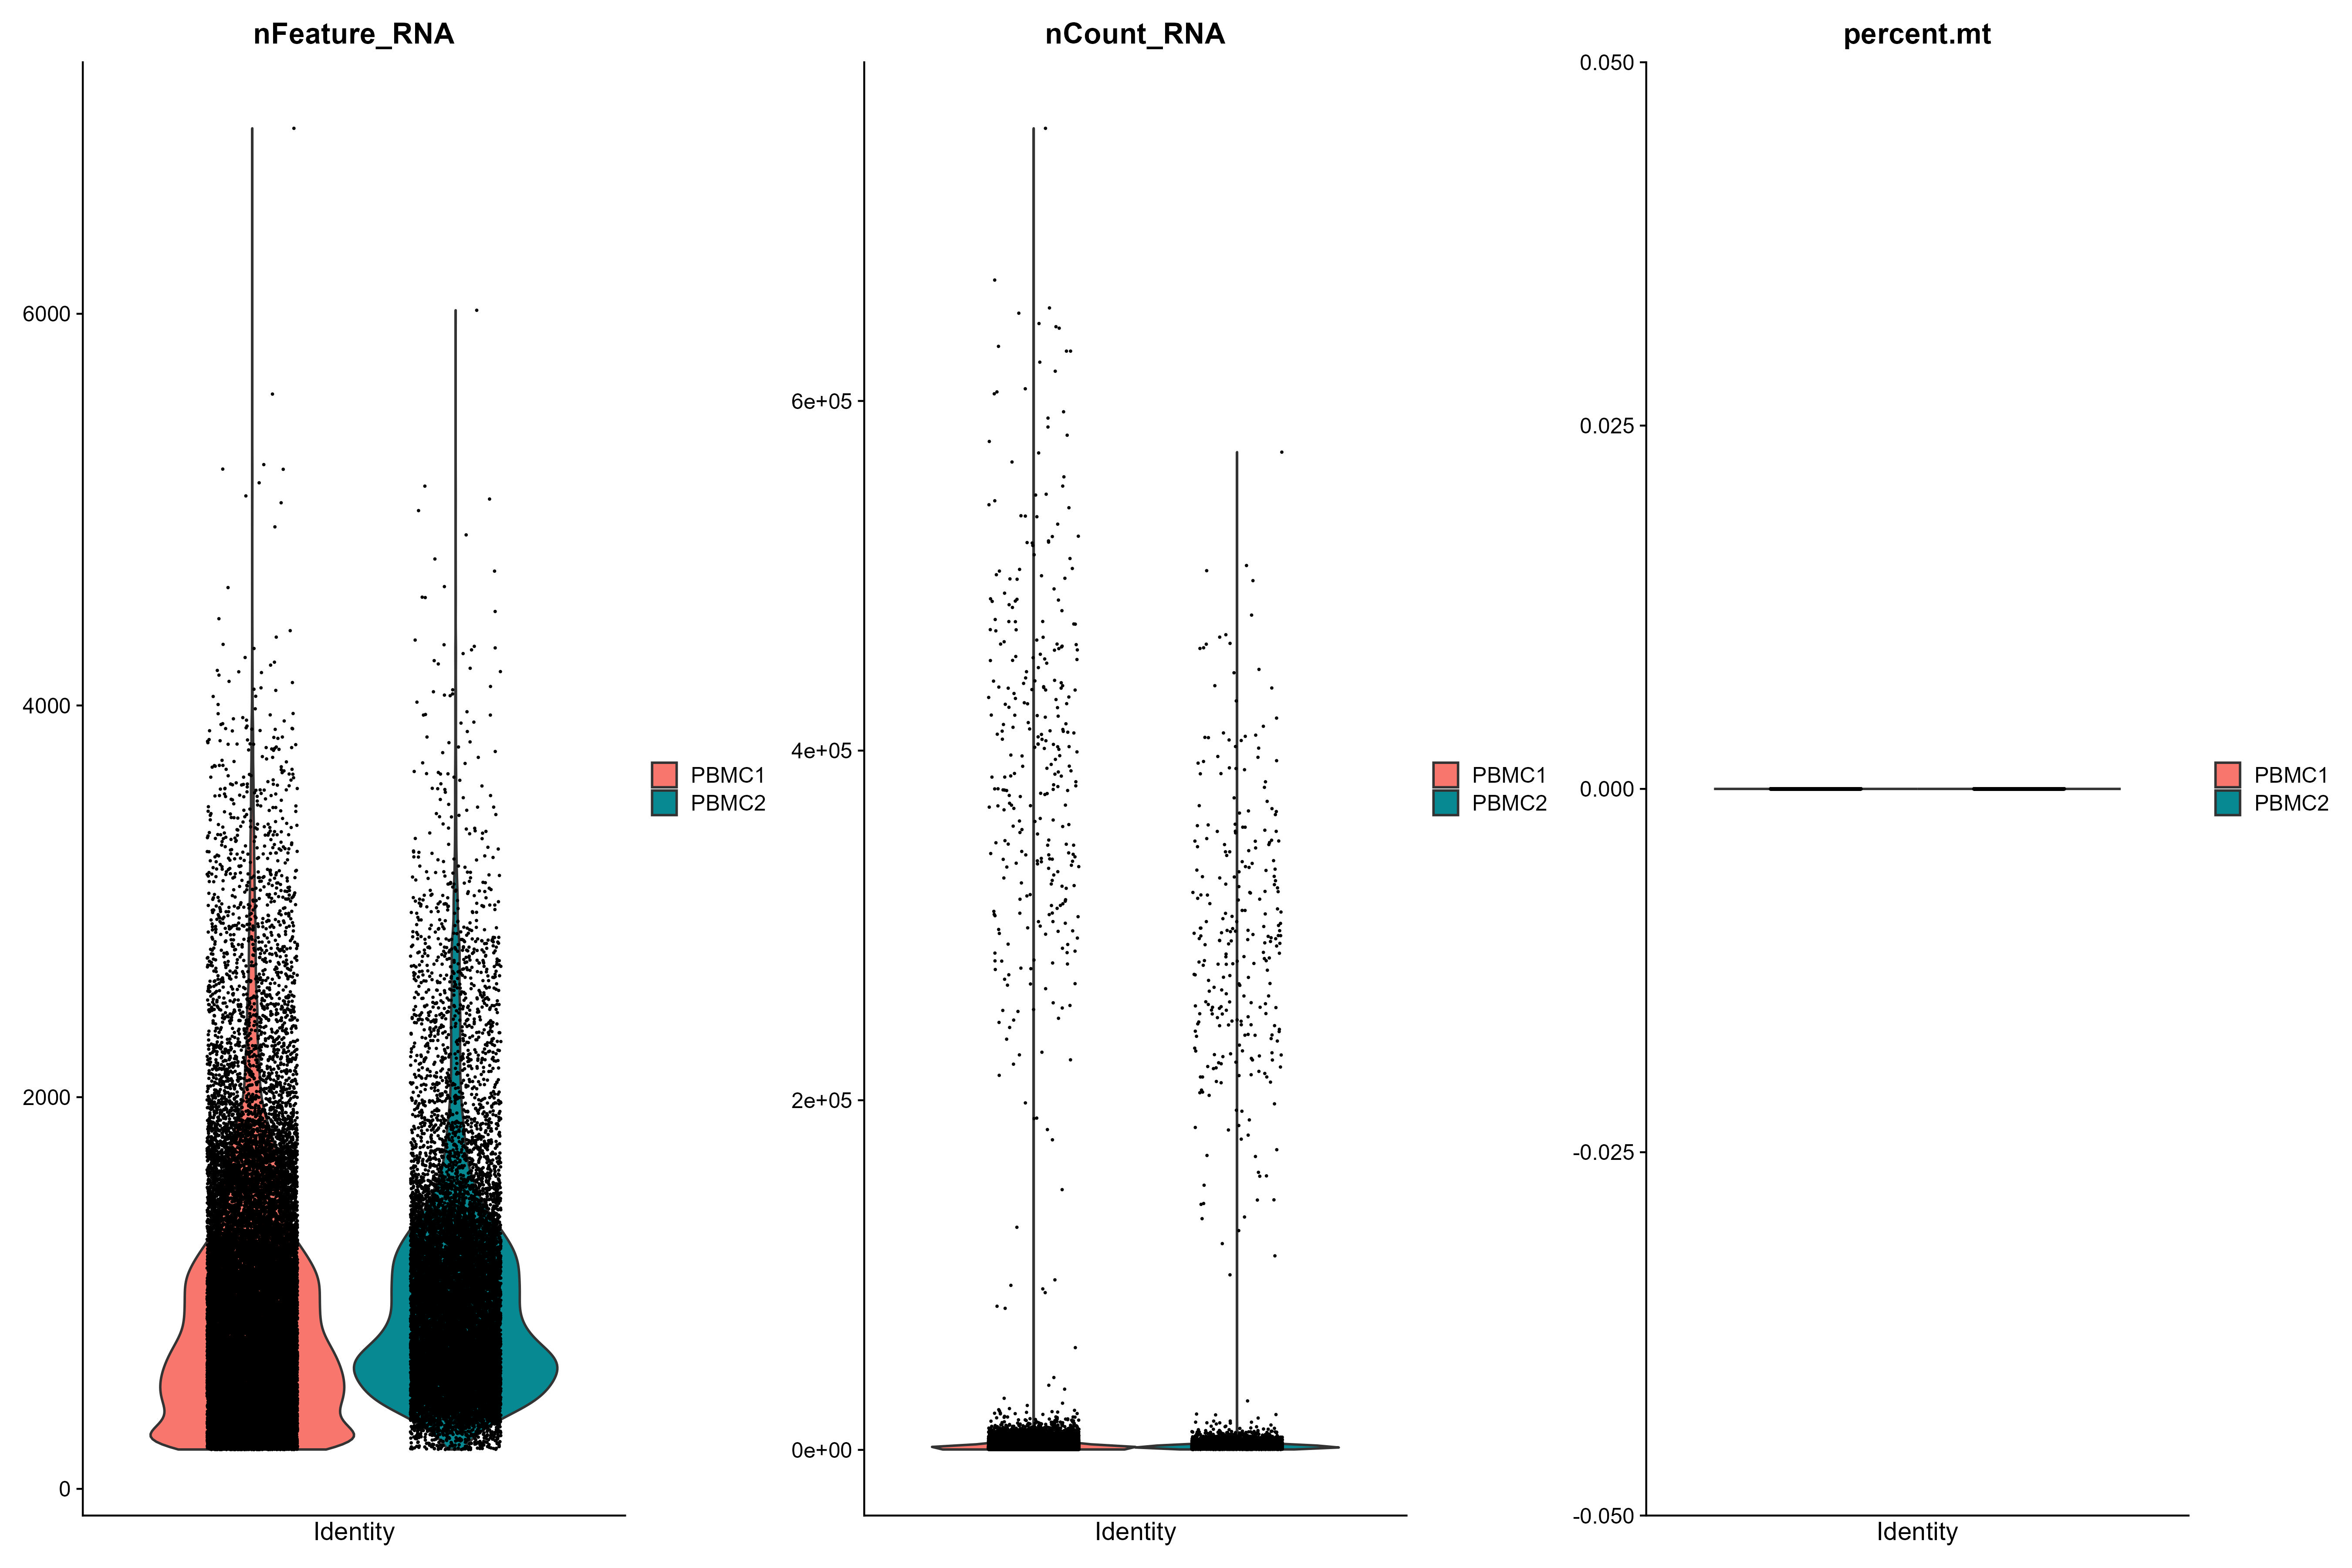
\includegraphics[width=0.48\textwidth]{Figures/post_qc_vplot.jpg}

\caption{Post-quality control visualizations after filtering.
Left: density plot showing the distribution of total RNA counts (\texttt{nCount\_RNA}) per sample after low-quality cells have been removed.
Right: violin plots summarizing gene counts, RNA counts, and mitochondrial content in the filtered dataset.}
\label{fig:post_qc_plots}
\end{figure}


\section{Step 4 -- Remove doublets}

\textbf{Purpose.}  
This step identifies and (optionally) removes \textit{doublets}—droplets that captured two cells instead of one. Doublets can look like “hybrid” cells and may create misleading clusters or false marker genes if not removed.

\textbf{What to do.}  
Provide an \textbf{Expected doublet rate} (usually based on how many cells were loaded/recovered in the 10x run). Then review the summary plot showing how many cells were labeled as singlets vs.\ doublets. If the results look reasonable, proceed with removing doublets.

\textbf{What Cellivista does.}
\begin{itemize}[leftmargin=*,nosep]
\item Scores each cell for how strongly it resembles an artificial “two-cell mixture” profile.
\item Labels cells as \textbf{Singlet} or \textbf{Doublet} using the expected doublet rate you provide.
\item Summarizes the results visually so you can confirm the outcome before moving forward.
\item Optionally removes predicted doublets and keeps only singlets for downstream analysis.
\end{itemize}

\textbf{Why the \textit{Expected doublet rate} is required.}  
\textbf{DoubletFinder} does not automatically decide how many doublets exist in your dataset. Instead, it ranks cells by a doublet-likeness score and then assigns the top cells as doublets based on the \textbf{expected number of doublets} (\texttt{nExp}). In other words, the expected doublet rate determines \textit{how many cells will be labeled as doublets}. 

\textbf{What “Expected doublet rate” means in practice.}
\begin{itemize}[leftmargin=*,nosep]
\item It is the estimated fraction of droplets that contain more than one cell.
\item This fraction increases as more cells are loaded onto a 10x run (higher throughput generally means higher multiplet rates).
\item Cellivista uses this rate to compute an expected number of doublets (approximately: \textit{rate} $\times$ \textit{cells recovered}), which directly controls how many cells are labeled as doublets by \textbf{DoubletFinder}. 
\end{itemize}

\textbf{How to interpret the plot.}  
The barplot generated in this step reflects your chosen expected doublet rate: a higher expected rate will generally label more cells as doublets, and a lower rate will label fewer. Use this plot as a quick sanity check that the singlet/doublet split matches expectations for your experiment.

\textbf{Additional options.}
\begin{itemize}
  \item \textbf{Load Seurat object from \texttt{.rds}:} Allows the doublet-removal step to start from an uploaded Seurat object instead of the object currently stored in the app session.
  \item \textbf{Save plots:} Enables export of DoubletFinder UMAP plots and the singlet/doublet summary bar plot.
  \item \textbf{Plot export settings:} Users can customize filename prefixes, plot titles, output format (\texttt{jpeg}, \texttt{png}, or \texttt{svg}), and image dimensions.
\end{itemize}

\textbf{Output.}
This step produces a filtered Seurat object containing predicted singlets, downloadable DoubletFinder UMAP images, and a downloadable singlet/doublet count summary plot. The generated plot images are displayed in the app after the analysis is complete.

\begin{figure}[H]
\centering
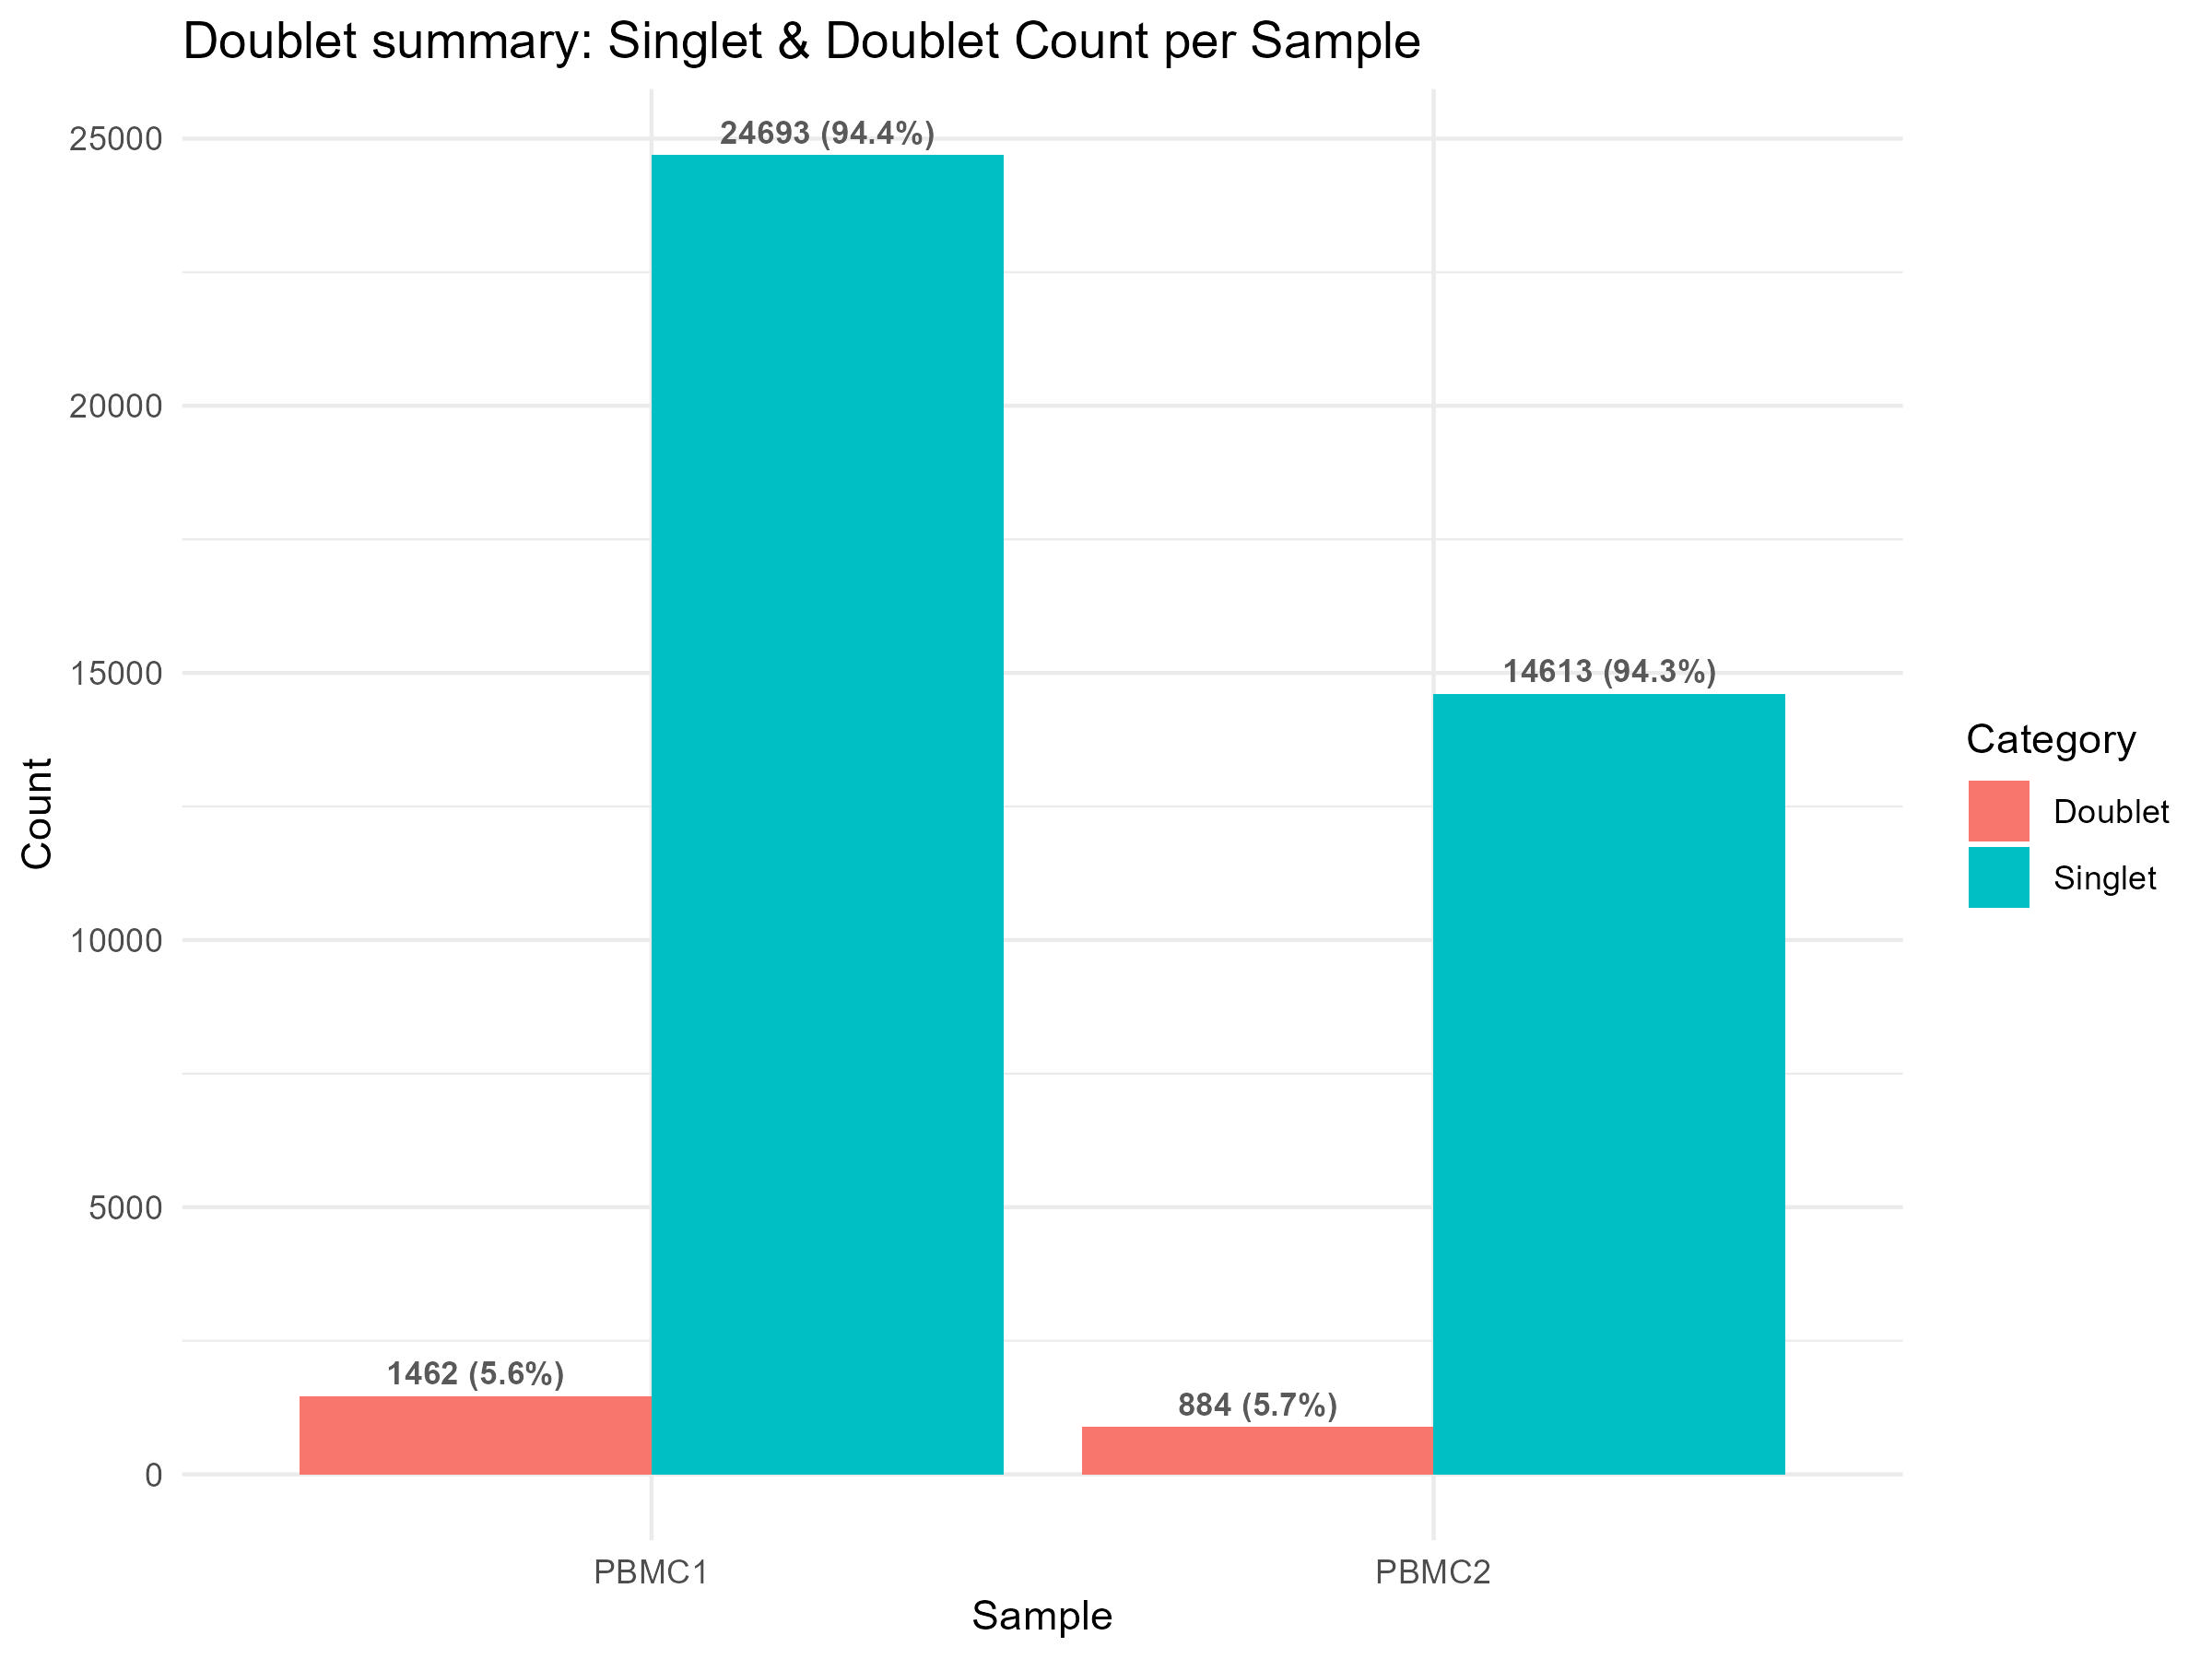
\includegraphics[width=0.4\textwidth]{Figures/singlet.doublet_count_barplot.jpeg}
\caption{Summary of predicted singlets and doublets per sample. The number of cells labeled as doublets is determined by the expected doublet rate provided by the user (used to set the expected number of doublets).}
\label{fig:doublet_barplot}
\end{figure}

\begin{figure}[H]
\centering
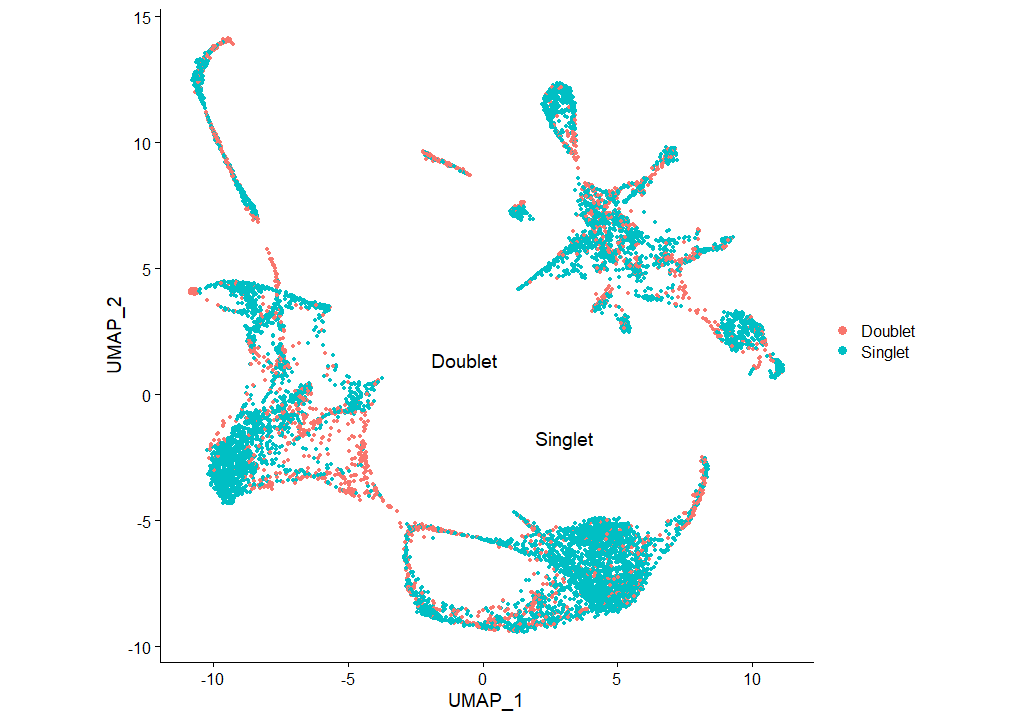
\includegraphics[width=0.6\textwidth]{Figures/DoubletRemoval_UMAP.png}
\caption{UMAP visualization of predicted singlets and doublets. Doublets often appear enriched at boundaries between clusters or in intermediate regions, reflecting mixed expression profiles.}
\label{fig:doublet_umap}
\end{figure}

\FloatBarrier

\section{Step 5 -- Integrate samples}

\textbf{Purpose.}  
When multiple samples are analyzed together, technical differences between experiments (often referred to as \textit{batch effects}) can cause cells from the same biological population to appear artificially separated. This step aligns samples into a shared reference space so that downstream analyses reflect biological variation rather than technical noise.

\textbf{What to do.}
If the dataset contains more than one sample, run the integration step to combine samples into a shared expression space. Users may either use the Seurat object already stored in the app session or upload a Seurat \texttt{.rds} object directly for integration.

\textbf{What Cellivista does.}
\begin{itemize}[leftmargin=*,nosep]
\item Identifies shared cell populations across samples that can be used as reference points for alignment.
\item Adjusts expression values to reduce technical differences between samples.
\item Normalizes each sample with SCTransform. This method is fixed.
\item Chooses the number of dimensions automatically: up to 30, and fewer when the smallest sample is too small.
\item Produces an integrated dataset that is used for all subsequent analyses.
\end{itemize}

\textbf{Key options explained.}
\begin{itemize}[leftmargin=*,nosep]
\item \textbf{Load Seurat object from \texttt{.rds}:} Allows integration to start from an uploaded Seurat object instead of the object currently stored in the app session.
\item \textbf{Number of integration features:} Controls how many informative genes are used to align samples. The default is 3000. Larger values may capture more biological variation but can increase computation time.
\item \textbf{Save plots:} Saves the UMAP grouped by samples, the UMAP split by samples, and the cell count pie chart. All three are selected by default, and each has its own export settings.
\end{itemize}

\textbf{Output.}  
An integrated dataset in which cells from different samples are aligned into a common reference space. This dataset is carried forward to downstream analysis steps, where visualization and clustering results will be generated. The integrated Seurat object can be downloaded as an \texttt{.rds} file.

\section{Step 6 -- Downstream analysis and visualization}

\textbf{Purpose.}  
This step performs the core analysis that reveals the structure of your single-cell dataset. Cells are grouped based on similarity in gene expression, visualized in low-dimensional space, and organized into clusters that often correspond to biological cell types or states.

\textbf{What to do.}  
Run the downstream analysis to generate dimensionality reduction plots and identify cell clusters. These results form the basis for interpretation, annotation, and differential expression analysis in later steps.

\textbf{What Cellivista does.}
\begin{itemize}[leftmargin=*,nosep]
\item Identifies highly informative genes that capture biological variation.
\item Reduces the complexity of the dataset to summarize each cell’s expression profile.
\item Groups cells into clusters based on shared expression patterns.
\item Generates two-dimensional visualizations that allow intuitive exploration of the data.
\end{itemize}

\textbf{How to interpret the plots.}
\begin{itemize}[leftmargin=*,nosep]
\item \textbf{UMAP plots} represent each cell as a point, with nearby points indicating similar gene expression profiles.
\item \textbf{Grouped UMAPs} show all samples together and are useful for examining overall cluster structure.
\item \textbf{Split UMAPs} display each sample separately in the same coordinate system, helping assess consistency across samples.
\item Distinct clusters often correspond to different cell types, while gradients may reflect continuous biological states.
\end{itemize}

\textbf{Key options explained.}
\begin{itemize}
  \item \textbf{Load Seurat object from \texttt{.rds}:} Allows downstream analysis to begin from an uploaded Seurat object instead of the object currently stored in the app session.
  \item \textbf{PCA/UMAP dimensions:} Determines which dimensions are used for UMAP, neighbor finding, and clustering.
  \item \textbf{Clustering resolution:} Controls cluster granularity. Lower values produce fewer, broader clusters; higher values yield more, finer clusters.
  \item \textbf{Select plots to save:} Users can choose whether to save the grouped UMAP, split UMAP, and cell-count pie chart.
  \item \textbf{Plot export settings:} Each selected plot has customizable filename, title, output format, width, and height.
\end{itemize}

\textbf{Output.}
This step produces a downstream-analyzed Seurat object, UMAP visualizations, cluster assignments, and a sample cell-count pie chart. Selected plots are displayed in the app and can be downloaded individually.


\begin{figure}[H]
\centering
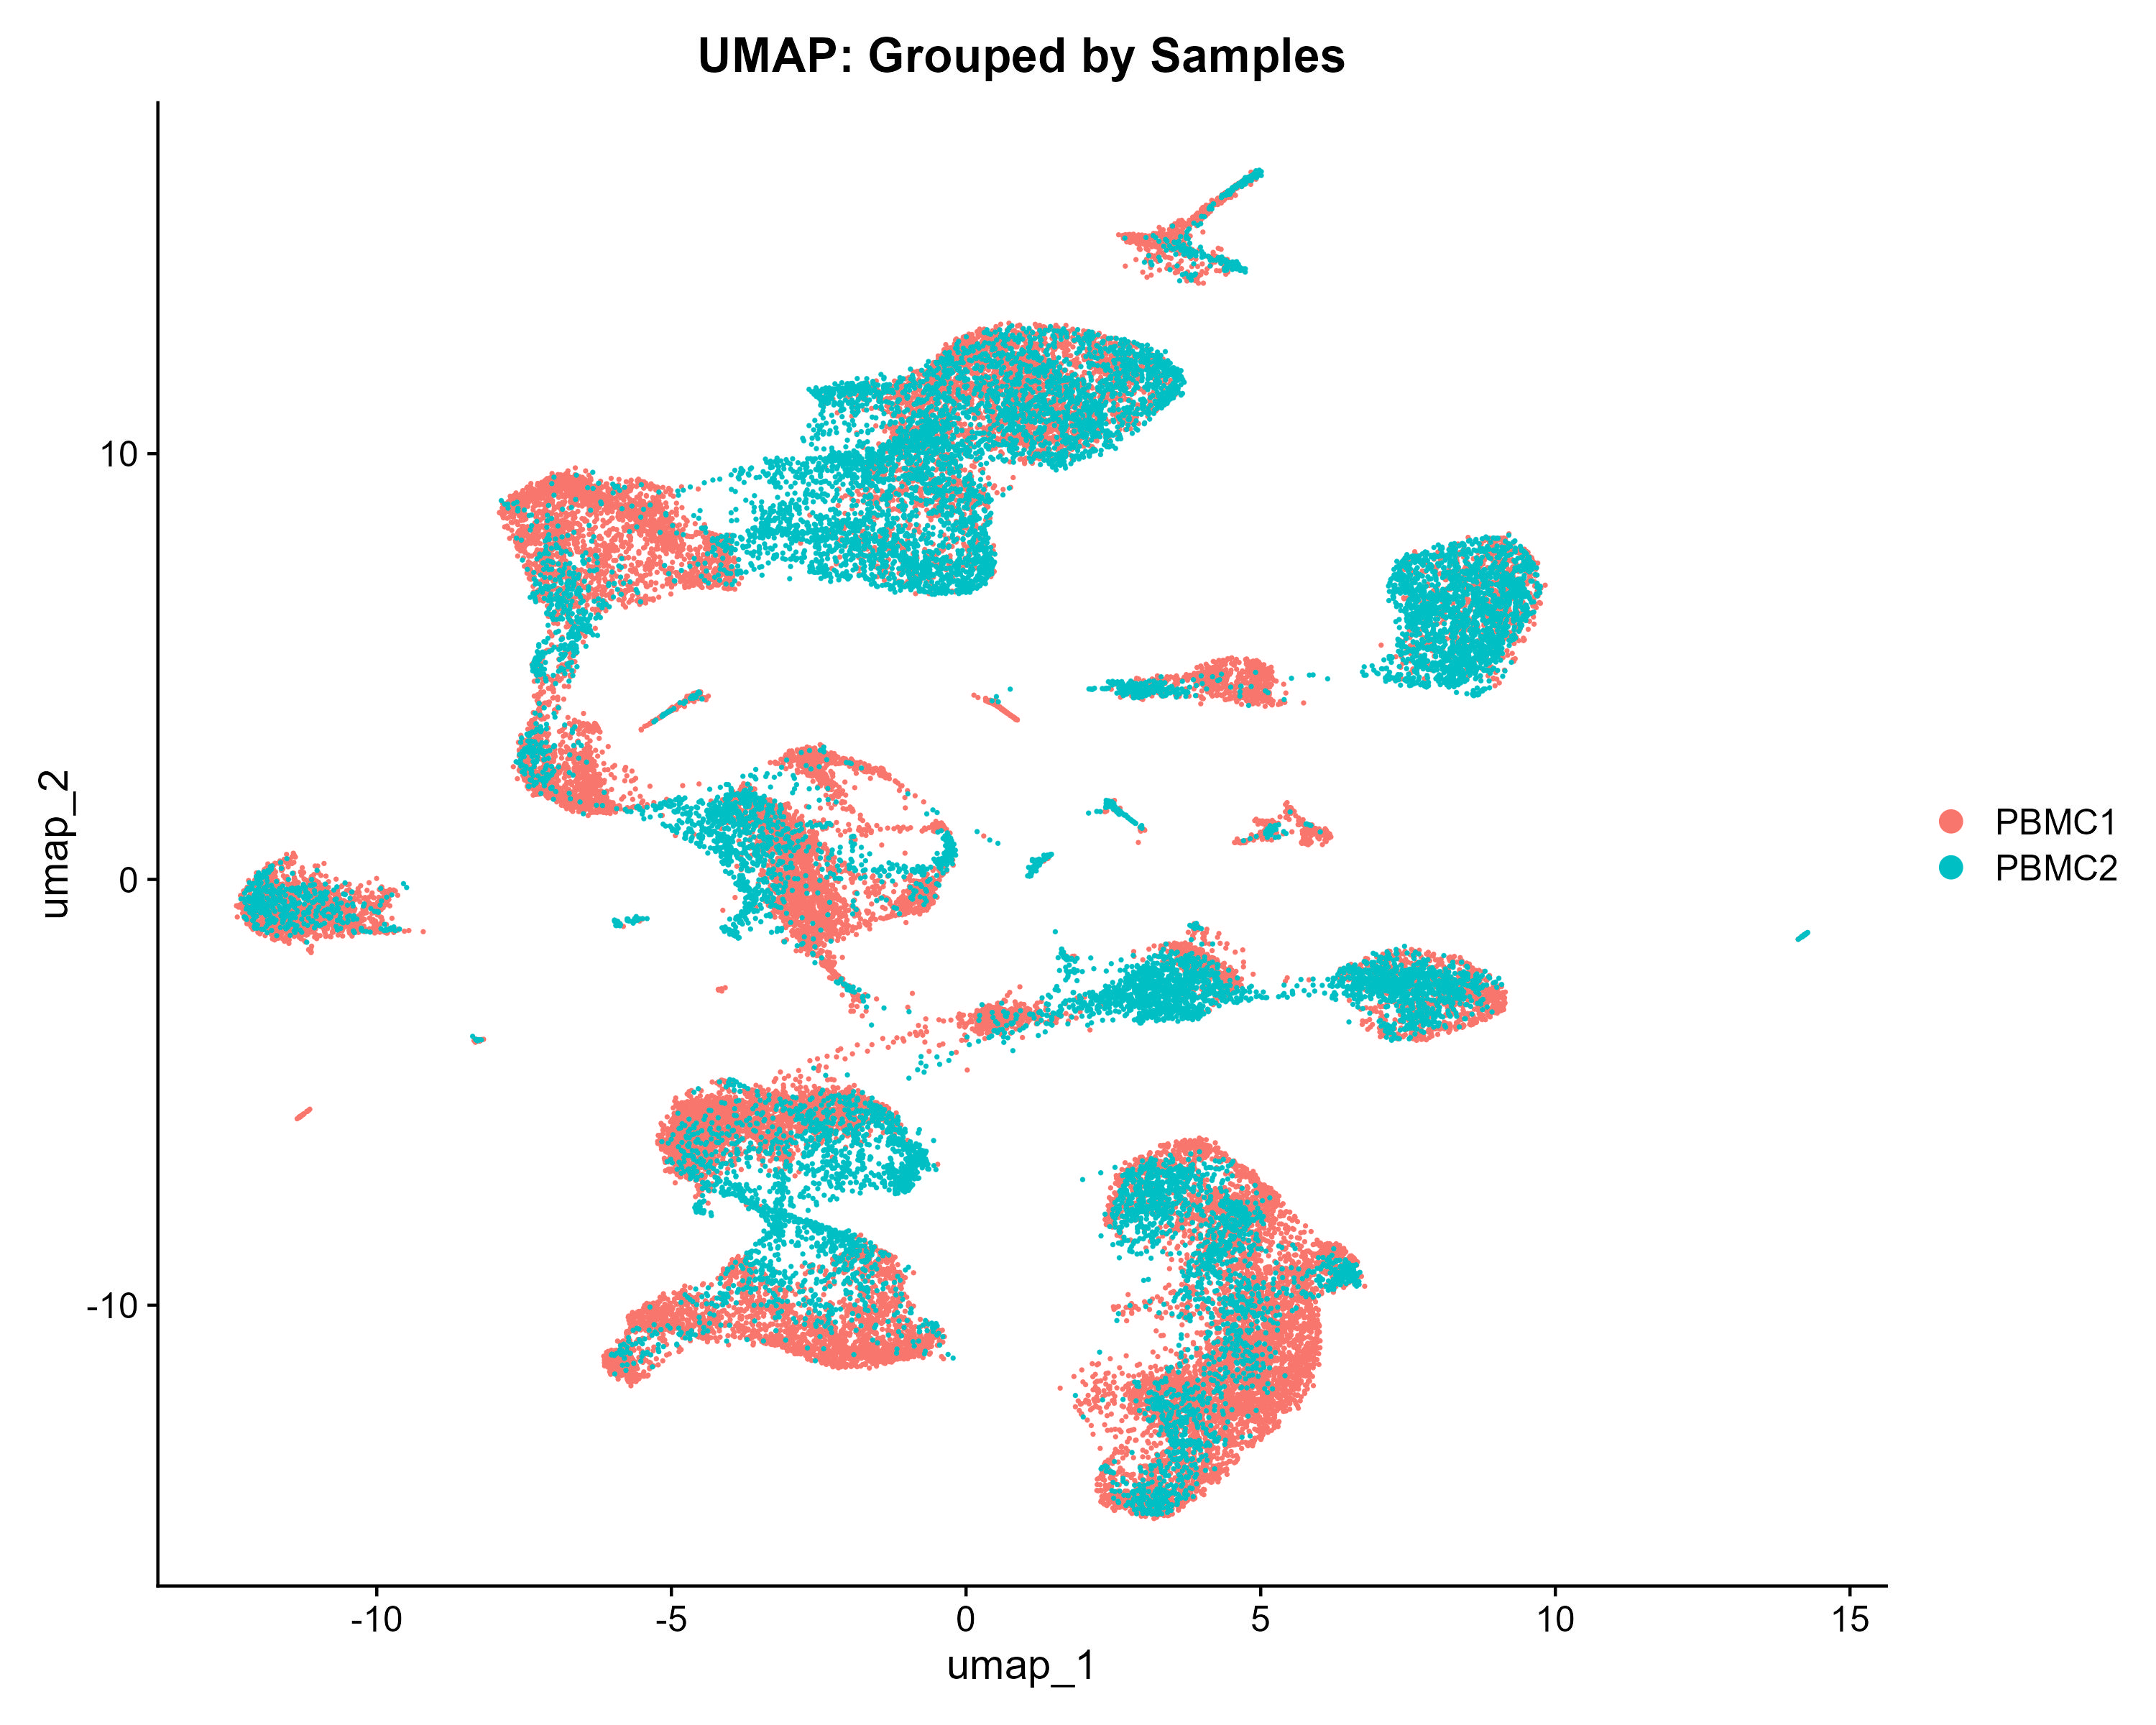
\includegraphics[width=0.55\textwidth]{Figures/integrated_umap_grouped.jpeg}

\vspace{0.5cm}

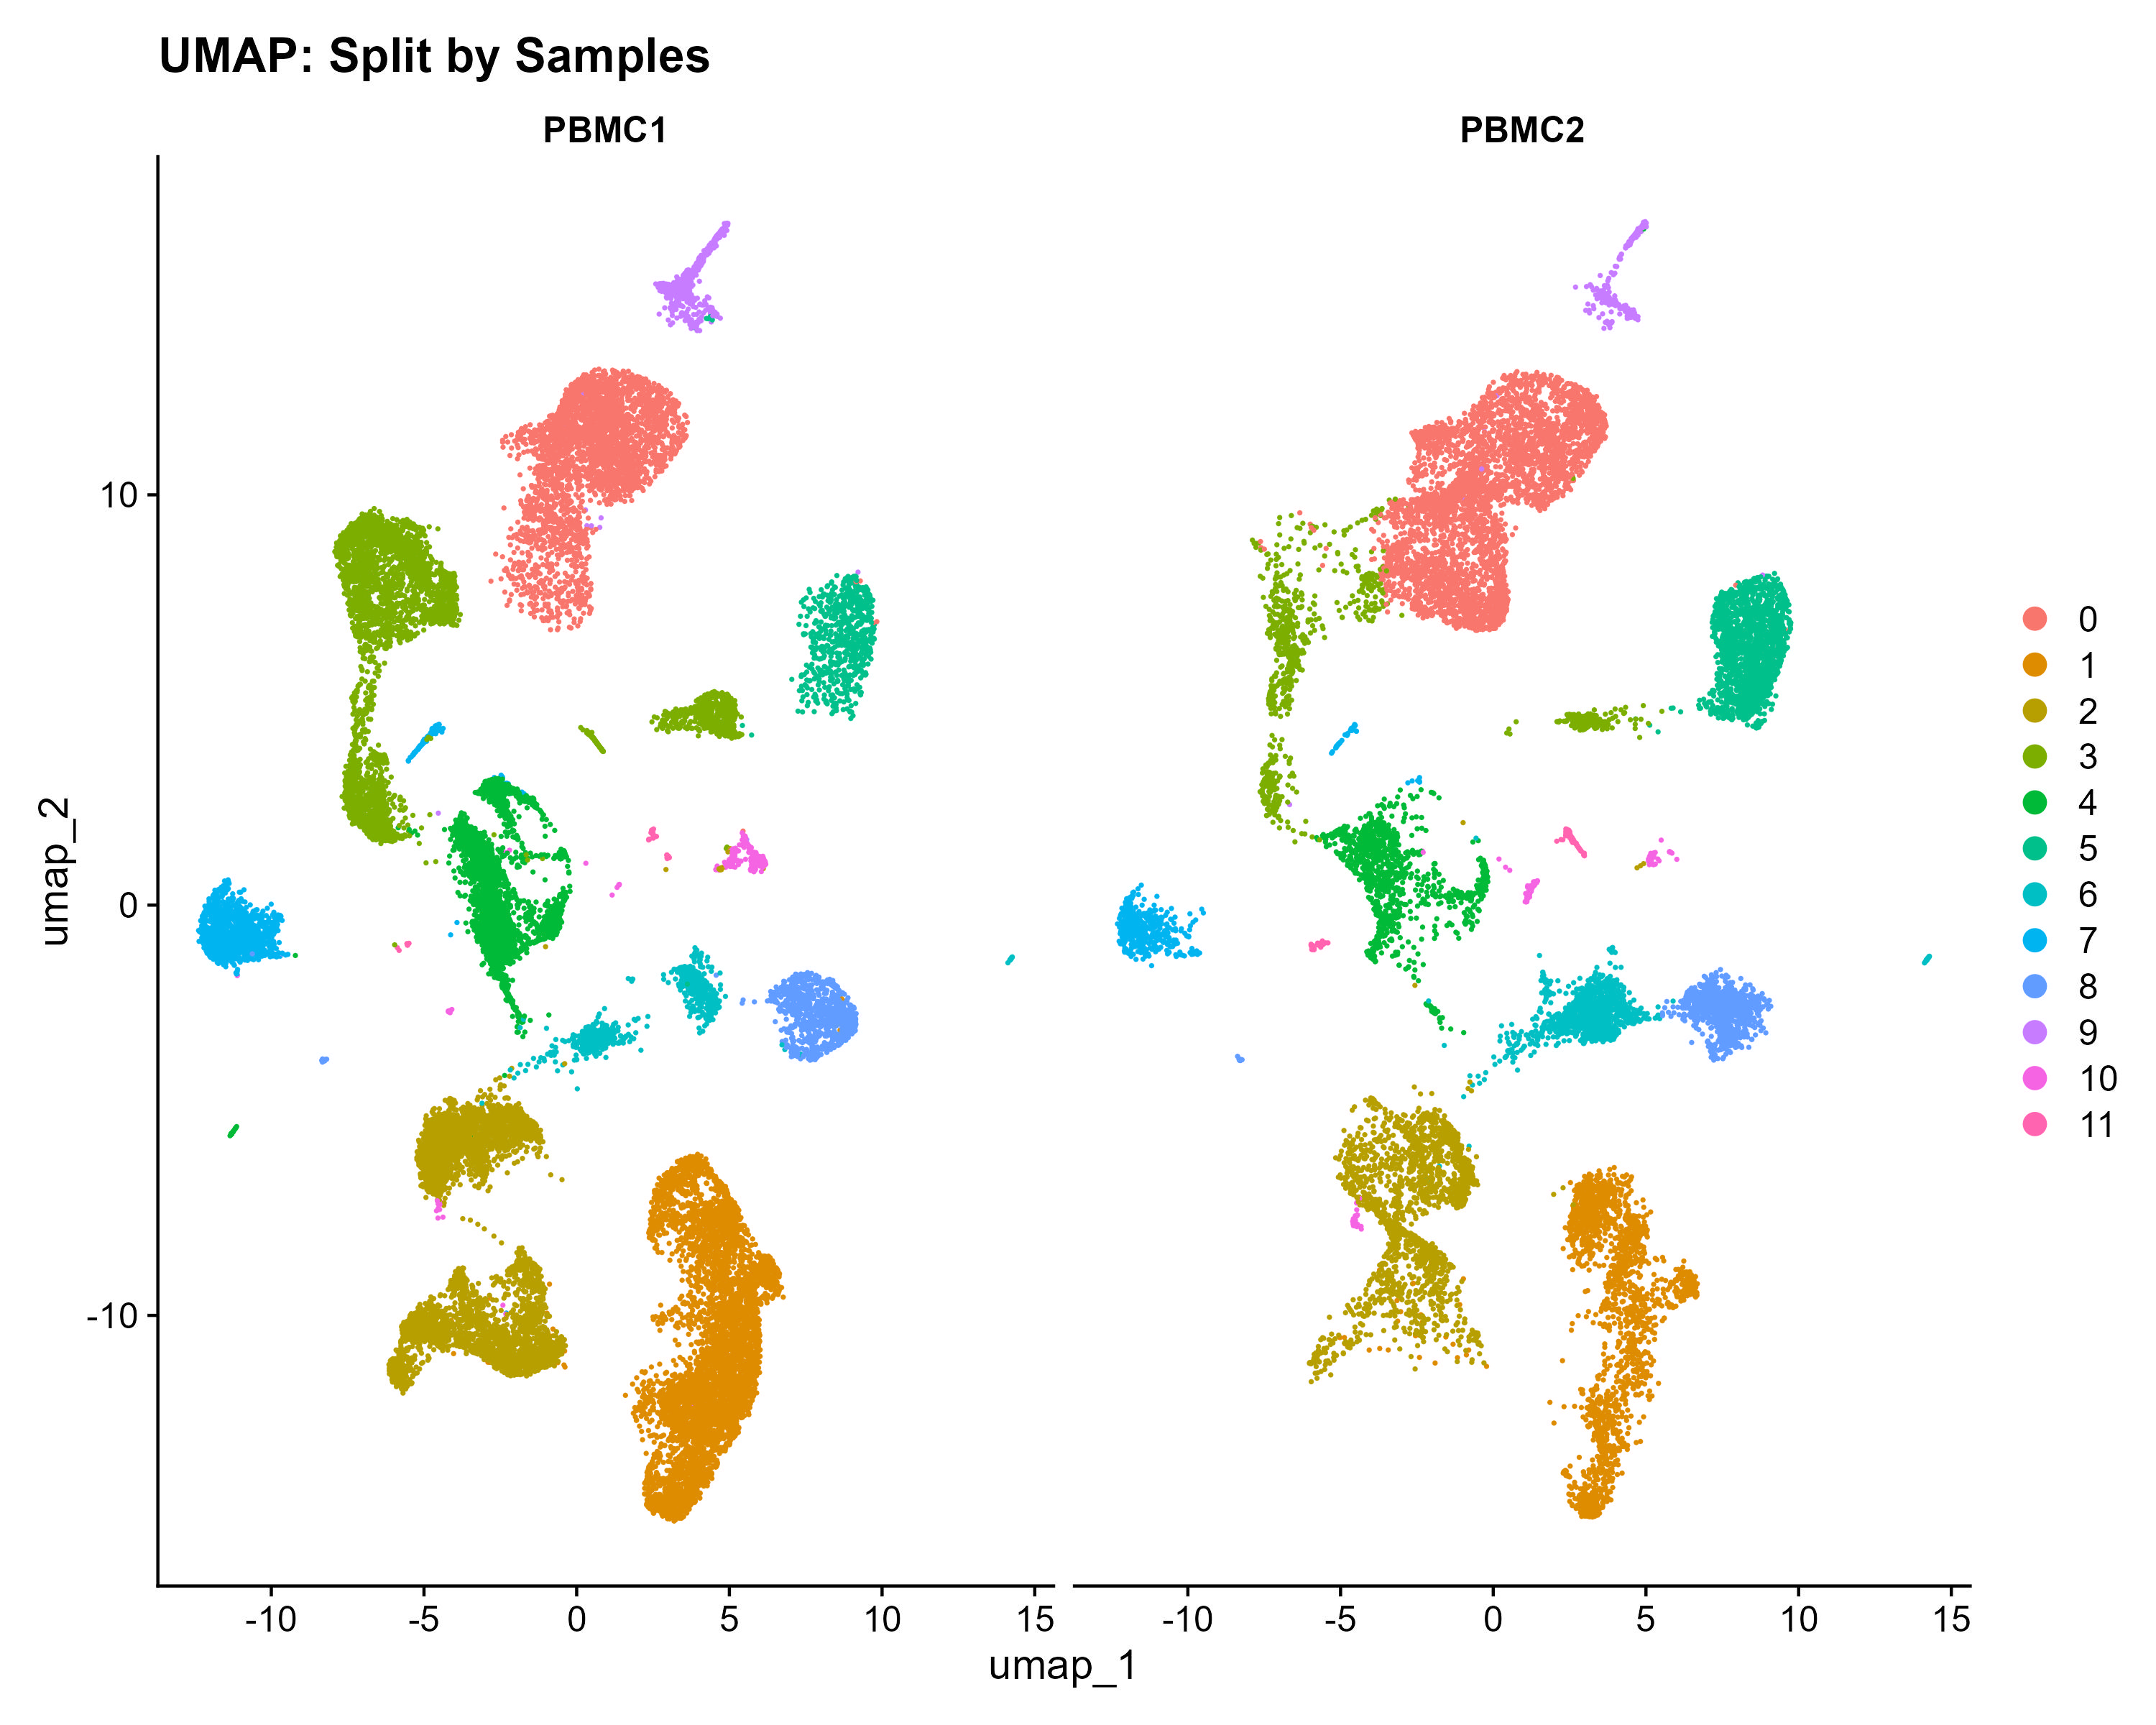
\includegraphics[width=0.55\textwidth]{Figures/integrated_umap_split.jpeg}

\caption{UMAP visualizations generated during downstream analysis.
Top: grouped view showing all samples together in a shared embedding.
Bottom: split view showing each sample separately, used to assess consistency of clustering across samples.}
\label{fig:downstream_umap}
\end{figure}

\begin{figure}[H]
\centering
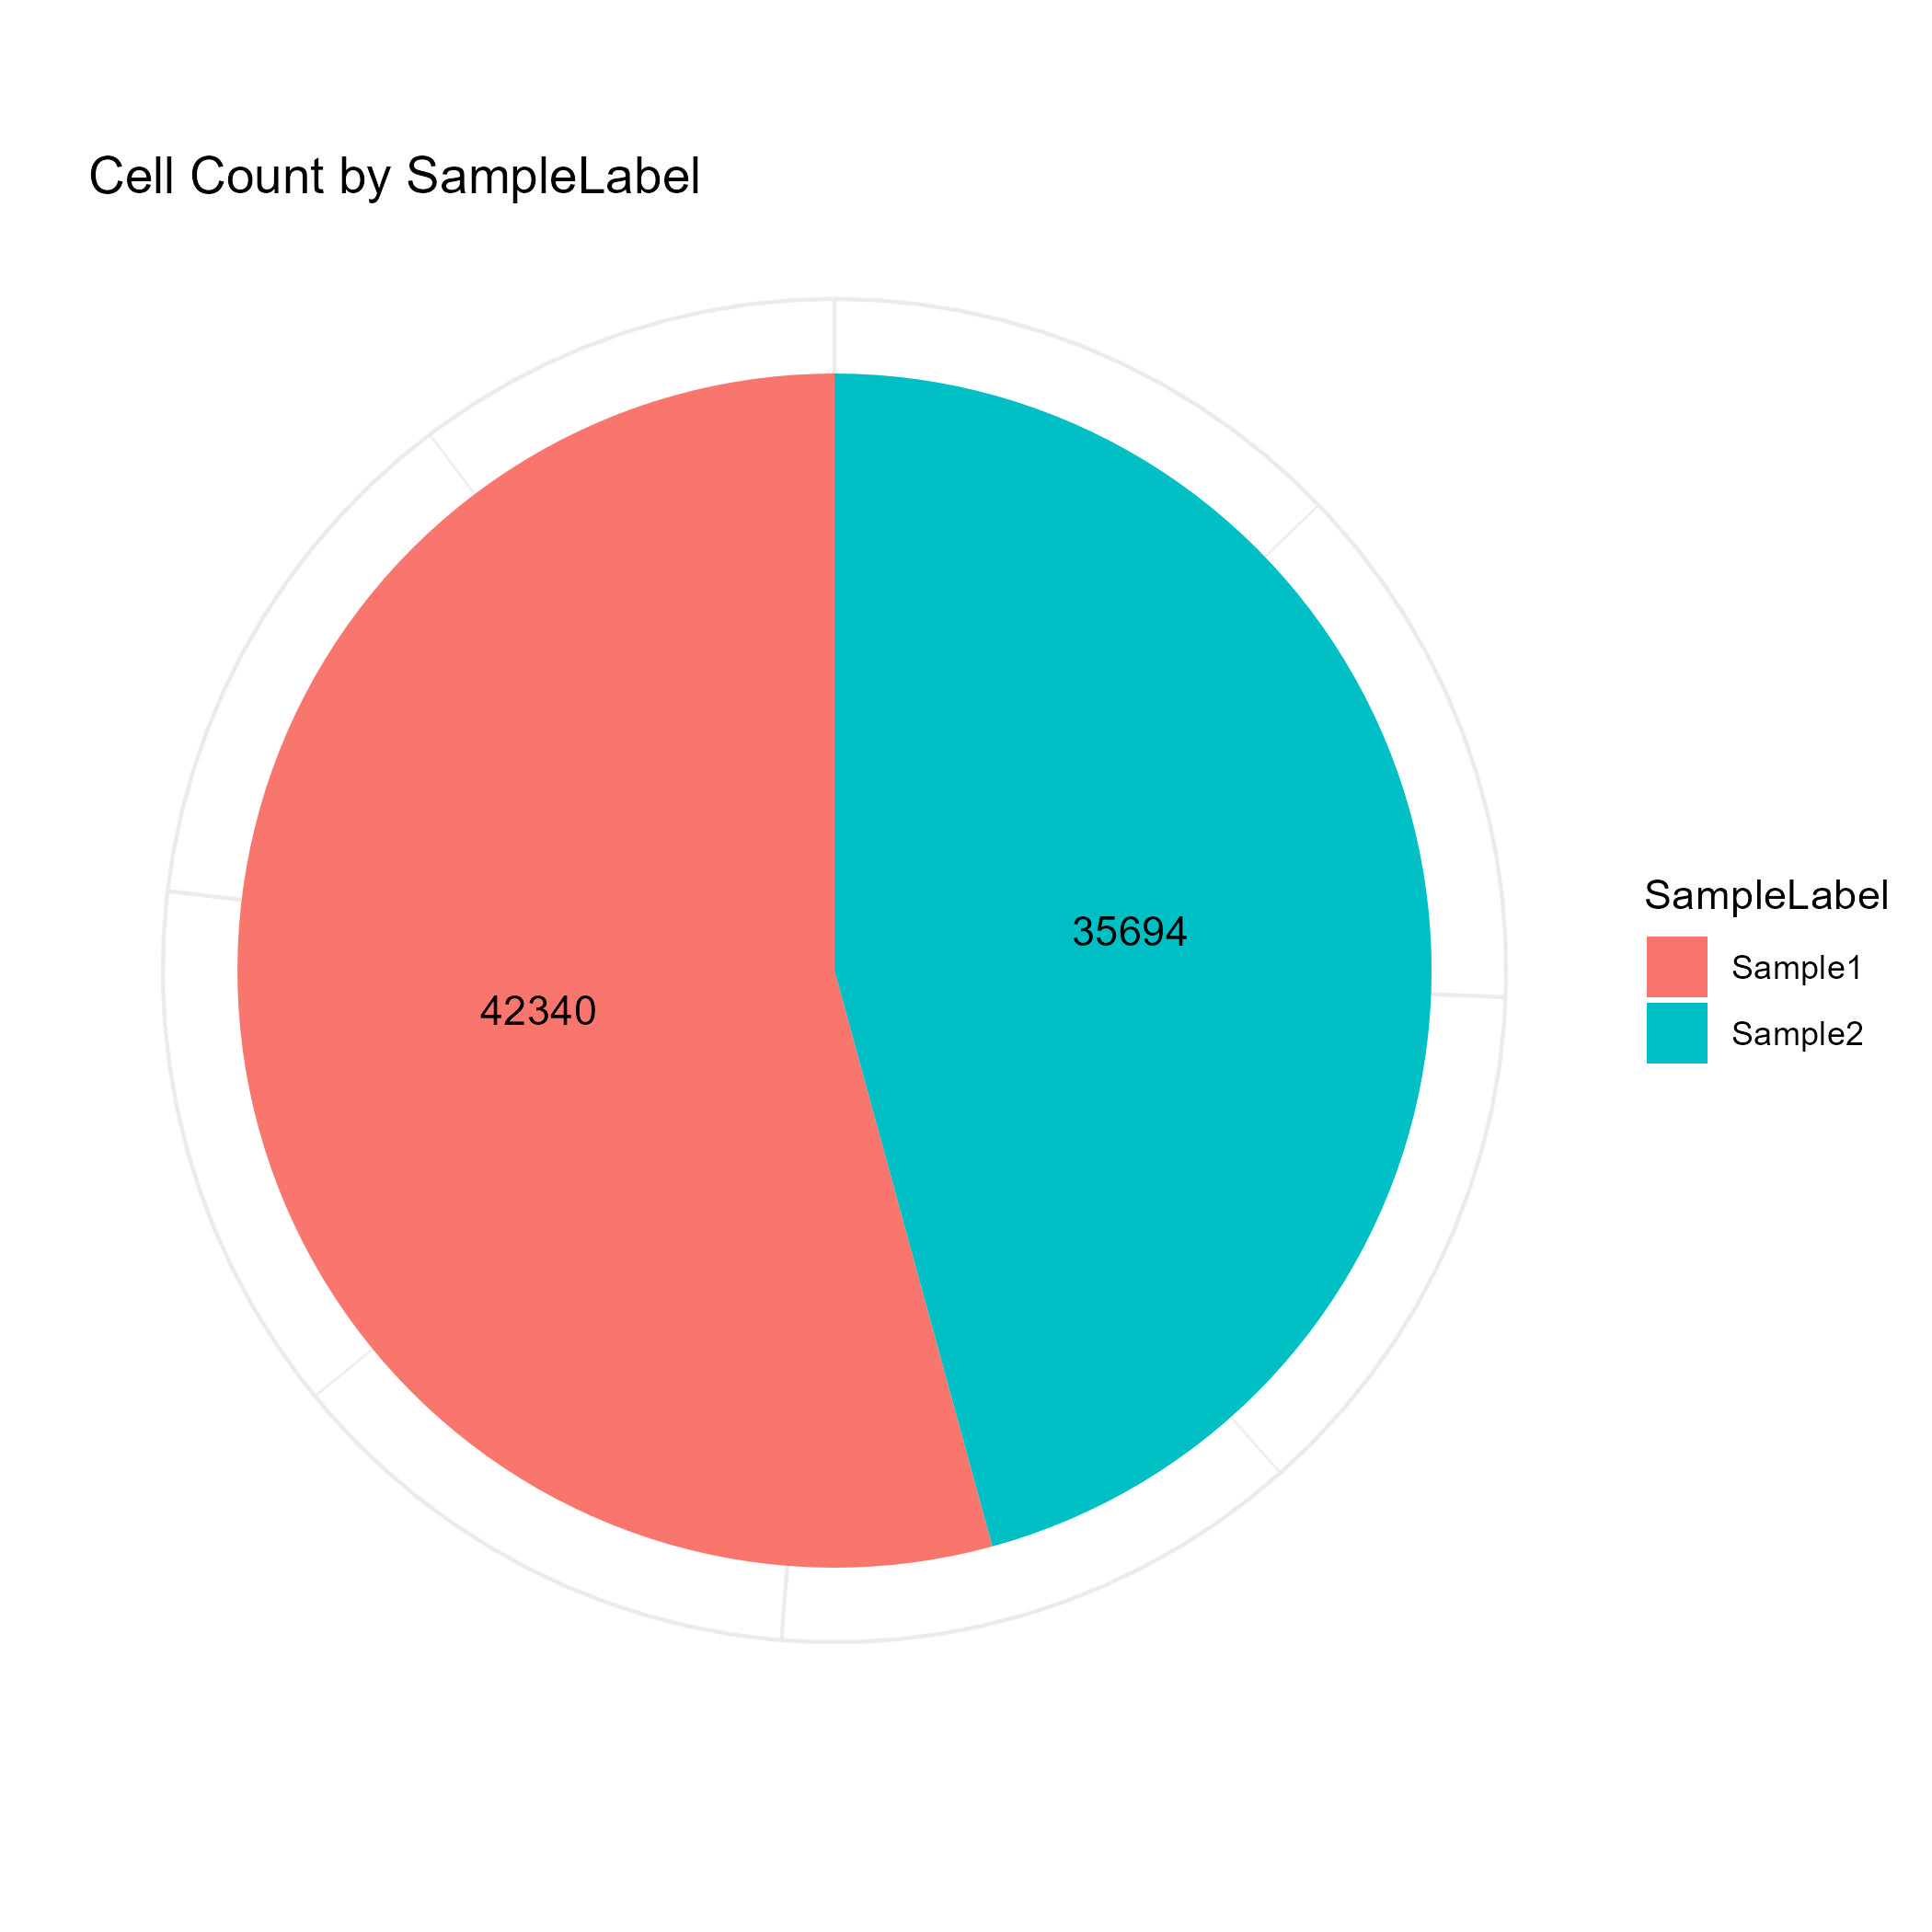
\includegraphics[width=0.5\textwidth]{Figures/cellcount_piechart.jpg}
\caption{Distribution of cells across samples after downstream analysis. The pie chart summarizes the relative contribution of each sample to the integrated dataset and provides a quick overview of sample balance.}
\label{fig:cellcount_pie}
\end{figure}

\begin{figure}[H]
\centering
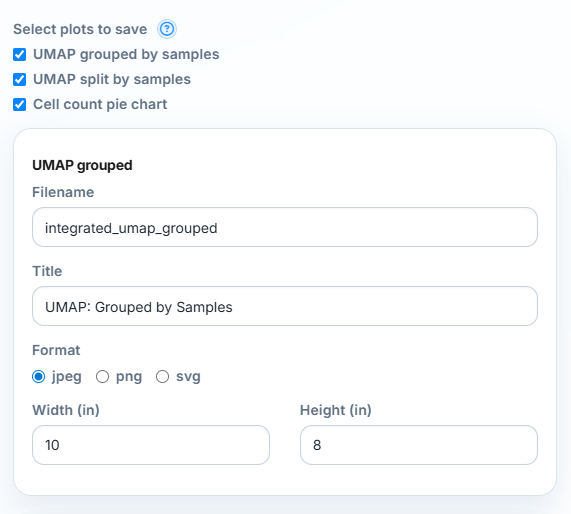
\includegraphics[width=0.5\textwidth]{Figures/downstream_plot_customization.png}
\caption{Plot export and customization options available in \emph{cellivista}. Similar controls are available across plot-generating tabs, allowing users to select visualizations, customize filenames and titles, choose output formats, and adjust image dimensions for publication or presentation.}
\label{fig:plot_customization}
\end{figure}
\FloatBarrier


\section{Step 7 -- Cluster-wise marker gene identification}

\textbf{Purpose.}  
This step identifies genes that are specifically enriched in each cluster. These \textit{marker genes} are essential for understanding the biological identity of clusters and for assigning cell type labels.

\textbf{What to do.}  
Run the marker detection step to compare each cluster against all others. Review the resulting gene lists and visualizations to determine which genes best characterize each cluster.

% Replace relevant DGEA method text in Section 9 Step 7 Cluster-wise marker gene identification

\textbf{What Cellivista does.}
\begin{itemize}
  \item Uses the \texttt{SCT} assay for cluster-wise marker detection.
  \item Prepares the object for SCT-based marker testing using \texttt{PrepSCTFindMarkers()}.
  \item Compares each cluster against all remaining cells using \texttt{FindAllMarkers()} with \texttt{only.pos = FALSE}.
  \item Identifies genes that are differentially expressed across clusters and ranks them by statistical evidence and effect size.
  \item Generates a full marker table and a top-marker summary table.
  \item Optionally generates violin plots, dot plots, and FeaturePlots for top markers.
\end{itemize}

\textbf{Key outputs explained.}
\begin{itemize}
  \item \textbf{All markers table:} A comprehensive table containing detected marker genes for every cluster, including expression levels, fold changes, and statistical significance.
  \item \textbf{Top markers table:} A simplified table listing the top positive marker genes for each cluster, intended for rapid inspection and annotation.
  \item \textbf{Dot plots:} Visual summaries showing how strongly and how frequently marker genes are expressed across clusters.
  \item \textbf{Feature plots:} UMAP-based visualizations showing where individual marker genes are expressed within the dataset.
  \item \textbf{Violin plots:} Distribution plots illustrating expression levels of marker genes across clusters.
\end{itemize}

\textbf{Key options explained.}
\begin{itemize}
  \item \textbf{Load Seurat object from \texttt{.rds}:} Allows marker detection to begin from an uploaded Seurat object.
  \item \textbf{Minimum percent expression:} Requires that a gene be detected in a minimum fraction of cells to be considered during marker testing.
  \item \textbf{LogFC threshold:} Filters genes based on the minimum log fold-change threshold.
  \item \textbf{Save plots:} Enables or disables marker-gene plot generation.
  \item \textbf{Choose plot types to save:} Allows users to select violin plots, dot plots, FeaturePlots, or any combination of these.
  \item \textbf{Plot export settings:} Users can customize filename prefixes, title prefixes, output format, width, and height for each plot type.
\end{itemize}

\textbf{Output.}
This step produces downloadable full and top-marker CSV files. When plot saving is enabled, Cellivista also displays and provides download buttons for the selected marker-gene plot images.

\begin{figure}[H]
\centering
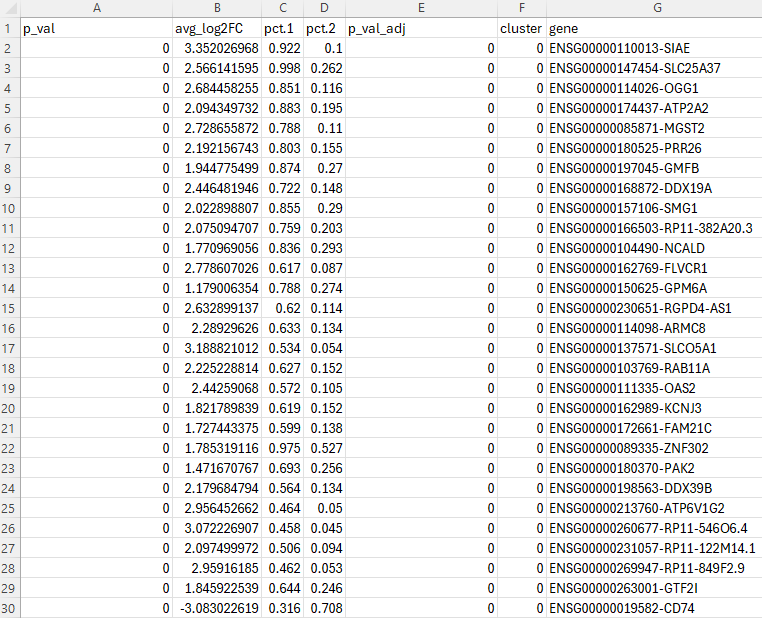
\includegraphics[width=0.25\textwidth]{Figures/all_marker.png}
\caption{Example of the full marker gene table generated during cluster-wise differential expression analysis. The table lists all detected marker genes across clusters along with expression statistics and significance values.}
\label{fig:all_markers}
\end{figure}

\begin{figure}[H]
\centering
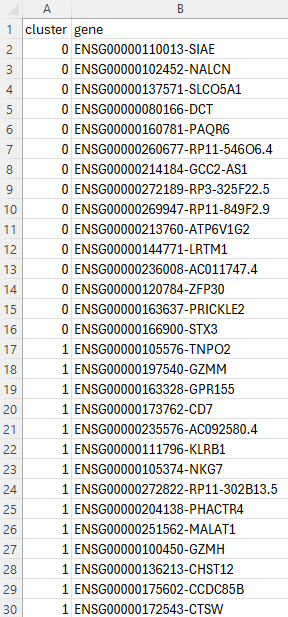
\includegraphics[width=0.2\textwidth]{Figures/top15_marker.png}
\caption{Example of the top 15 positive marker genes per cluster, ranked by average log2 fold change (\texttt{avg\_log2FC}). The table has two columns, \texttt{cluster} and \texttt{gene}. This summary table is commonly used for rapid inspection and cell type annotation.}
\label{fig:top15_markers}
\end{figure}
\FloatBarrier

\begin{figure}[H]
\centering
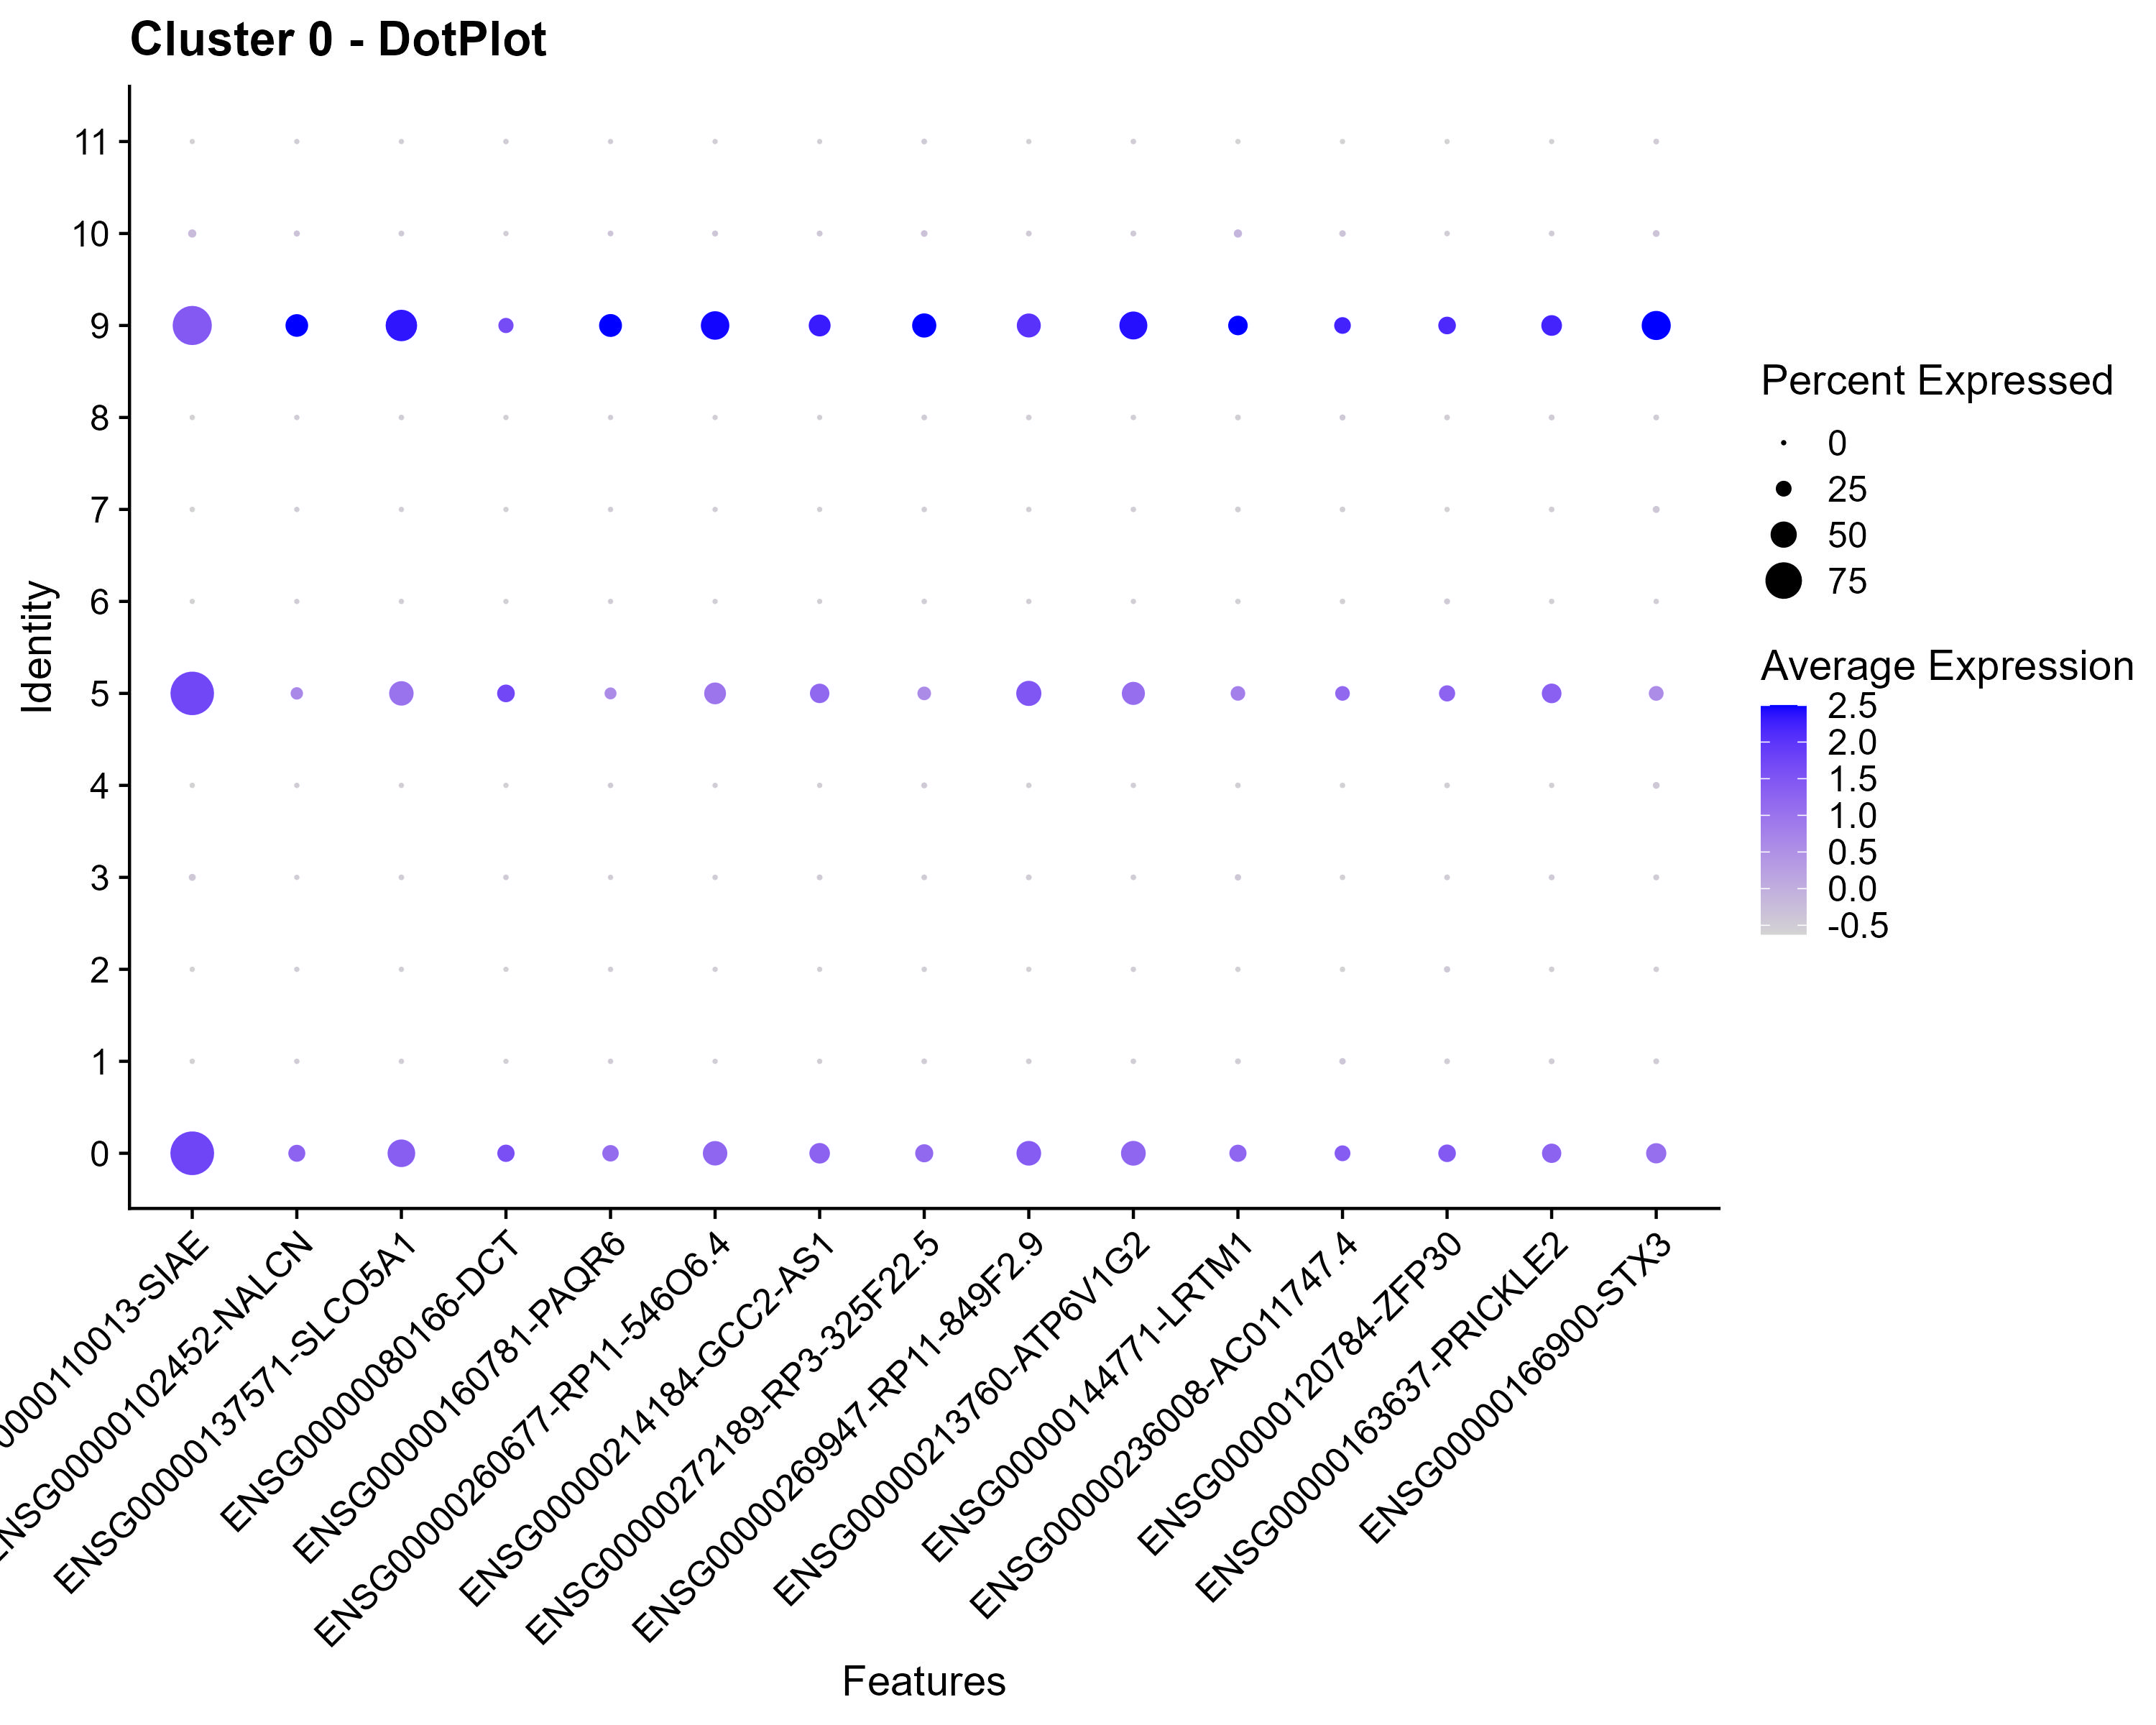
\includegraphics[width=0.5\textwidth]{Figures/dotplot_cluster0.jpeg}
\caption{Dot plot showing expression of the top marker genes for Cluster 0 across all clusters. Dot size reflects the fraction of expressing cells, while color intensity indicates average expression level.}
\label{fig:marker_dotplot}
\end{figure}
\FloatBarrier

\begin{figure}[H]
\centering
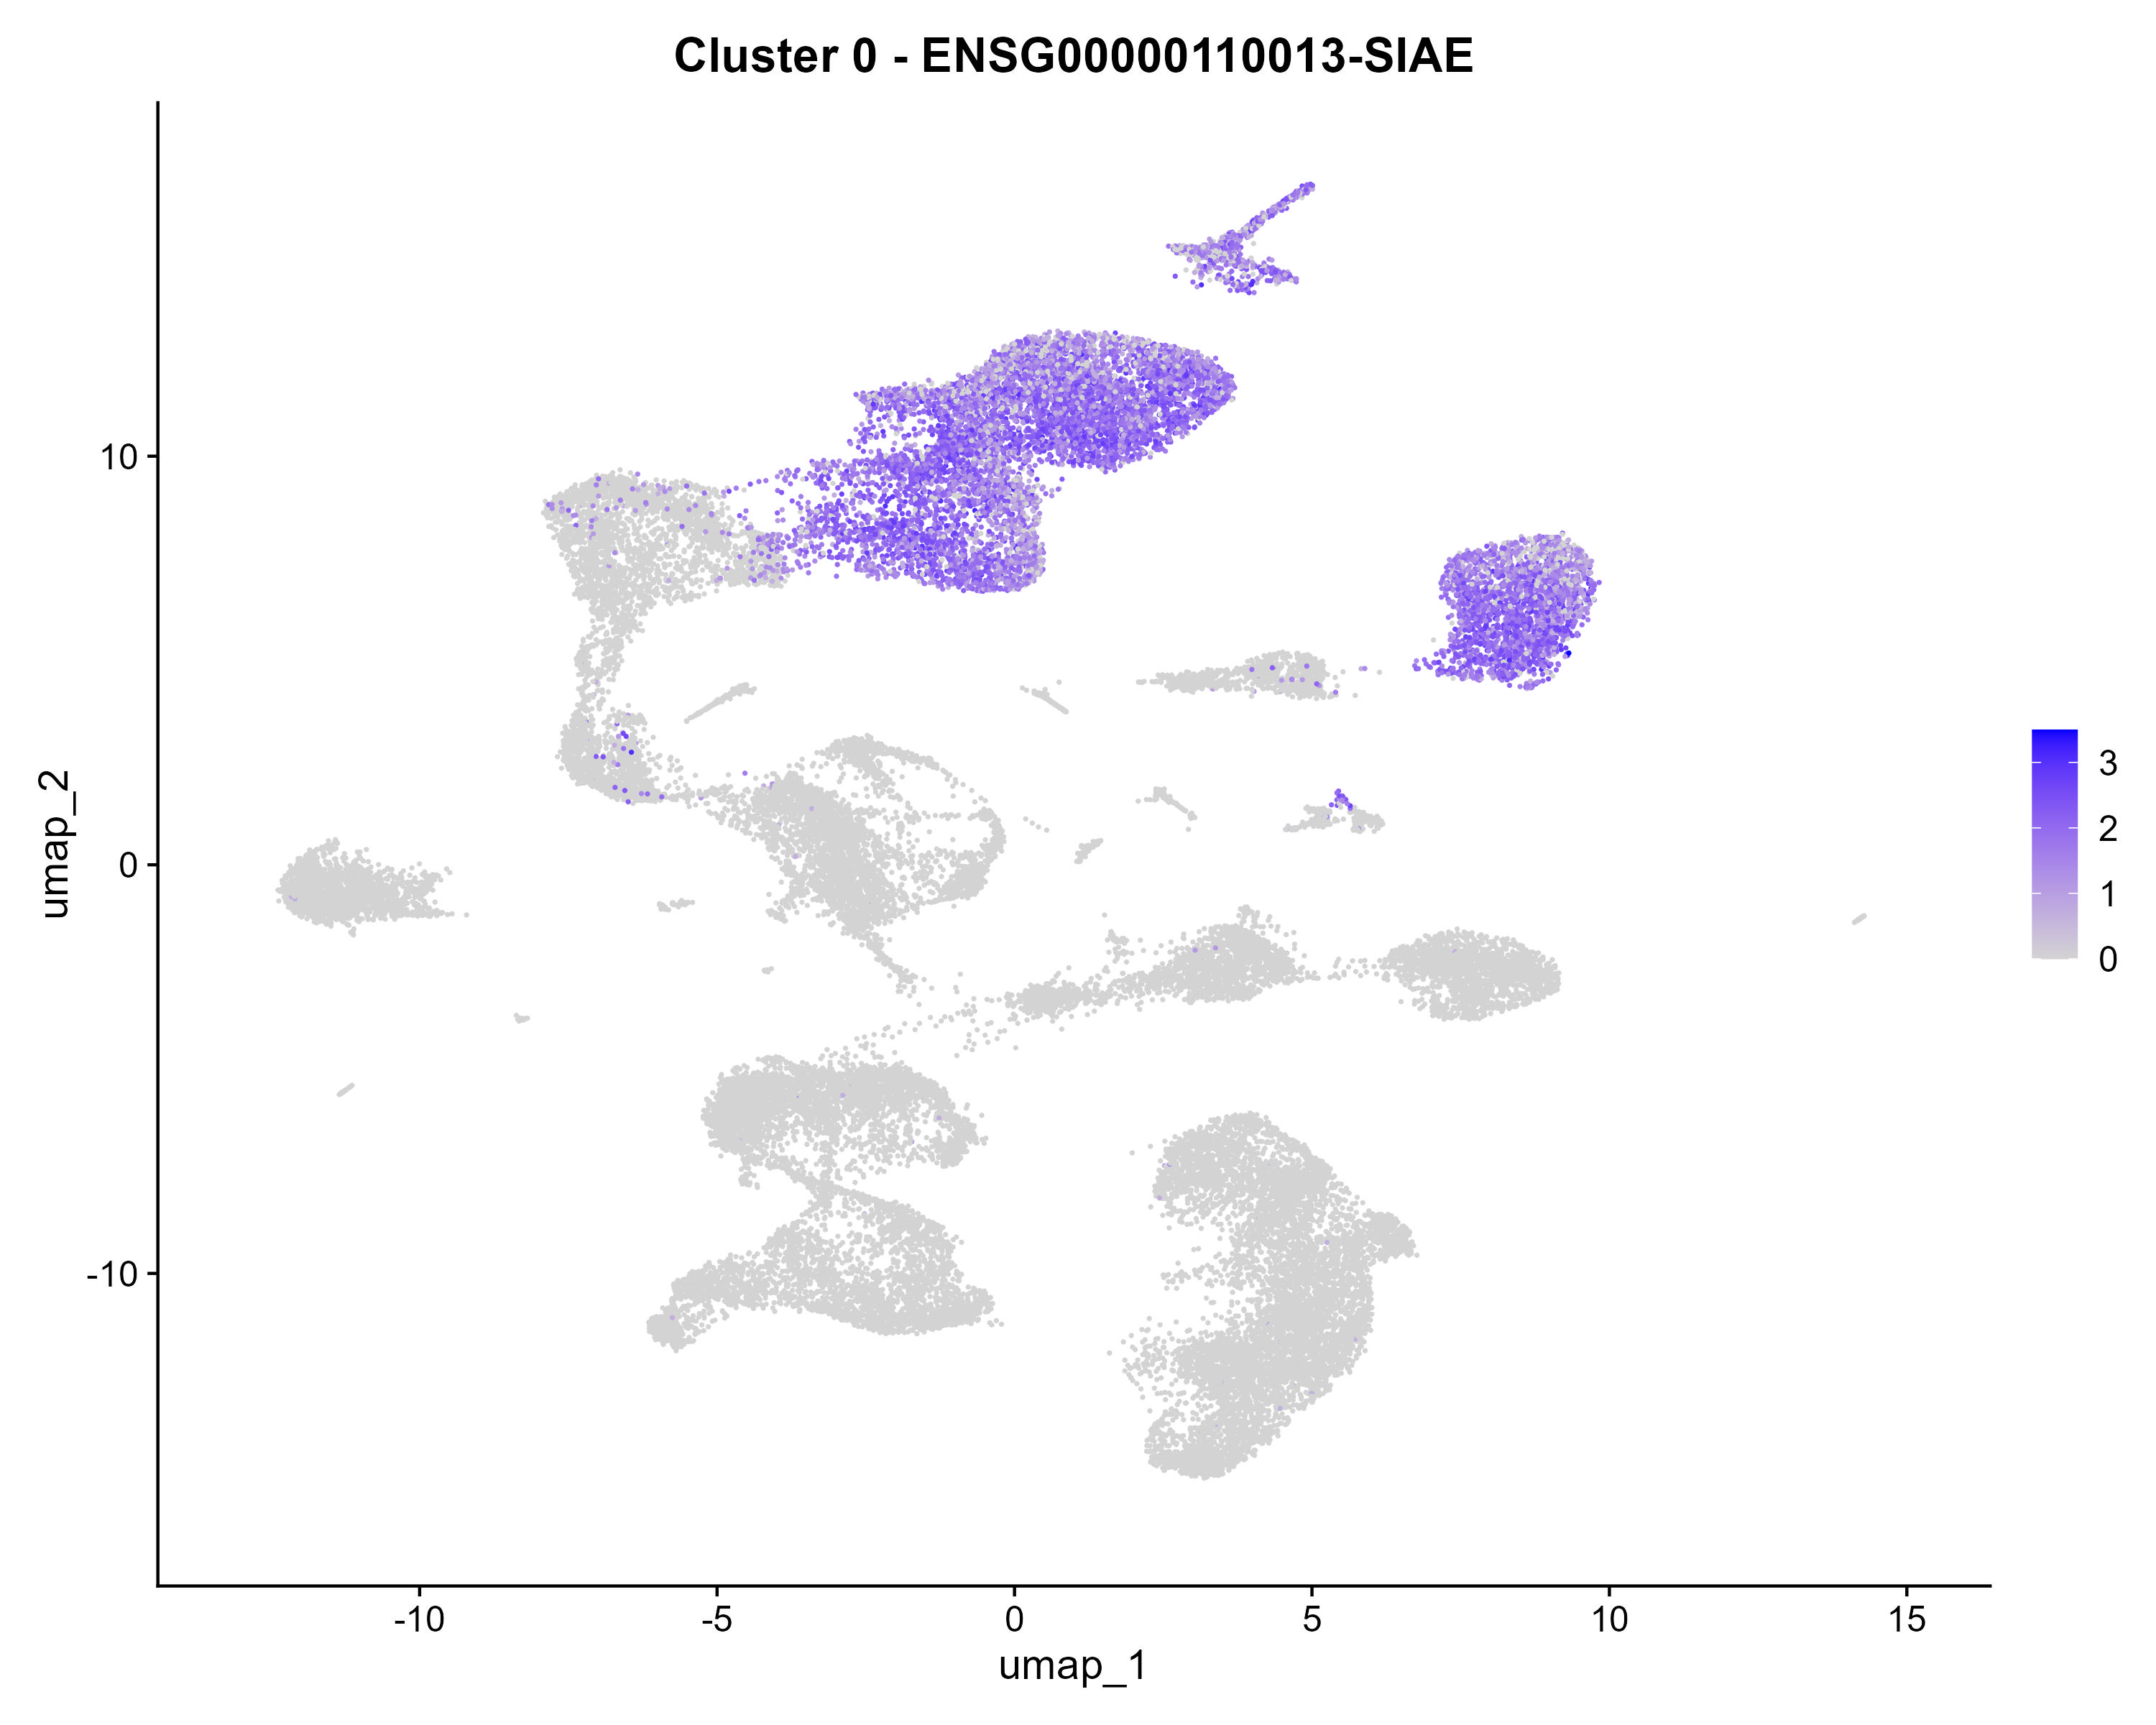
\includegraphics[width=0.5\textwidth]{Figures/featureplot_cluster0_ENSG00000110013-SIAE.jpeg}
\caption{Feature plot showing expression of the marker gene \textit{SIAE} within Cluster 0 projected onto the UMAP embedding.}
\label{fig:marker_featureplot}
\end{figure}
\FloatBarrier

\begin{figure}[H]
\centering
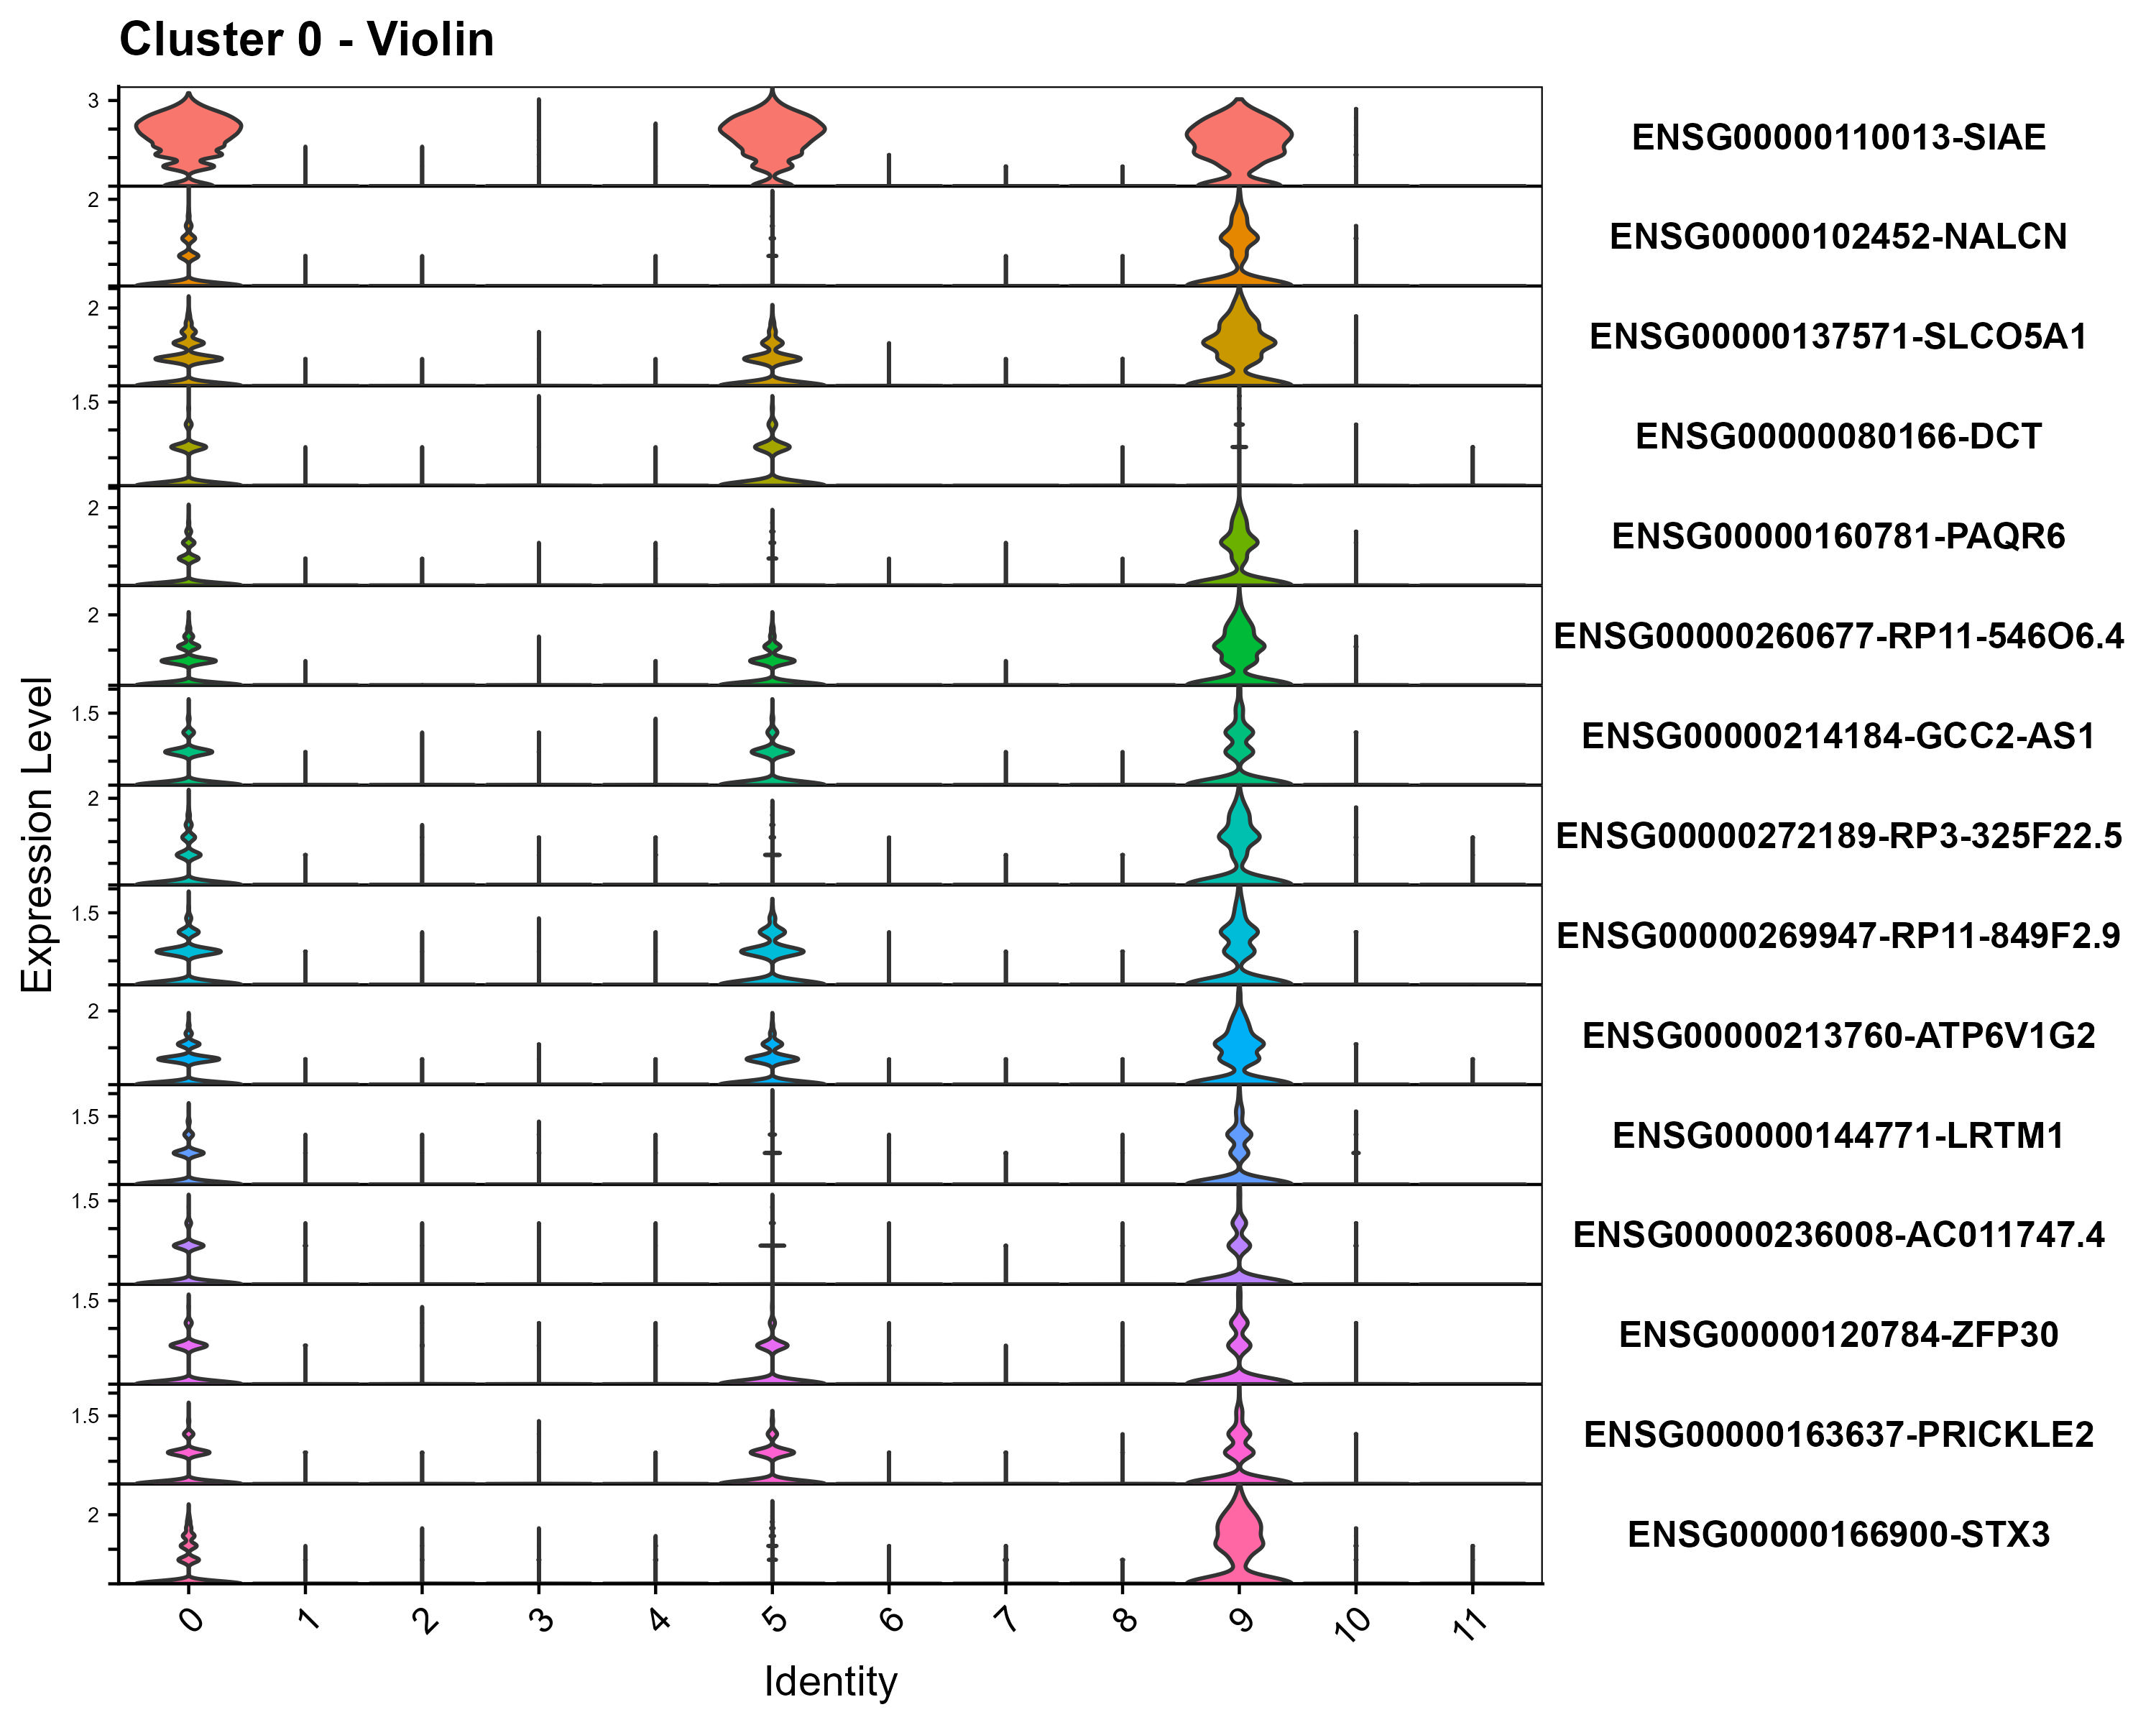
\includegraphics[width=0.5\textwidth]{Figures/violin_cluster0.jpeg}
\caption{Violin plots illustrating expression distributions of the top marker genes for Cluster 0 across all clusters.}
\label{fig:marker_violin}
\end{figure}
\FloatBarrier

Both marker tables can be reused in Step 10: upload \texttt{all\_marker.csv} or \texttt{top15\_marker.csv} in the Marker heatmap section of the Visualization Options tab (Section~\ref{sec:viz}).

\section{Step 8 -- Annotate clusters (assign cell types)}

\textbf{Purpose.}
After clusters are identified, the next goal is to assign a biological meaning to each cluster. This step converts numeric cluster IDs into interpretable cell type labels.

\textbf{What to do.}
Use the marker gene results from Step 7 to decide what each cluster represents. Then provide annotations in one of two ways: upload a CSV annotation file or manually enter comma-separated cell type labels in cluster order.

\textbf{Annotation input options.}
\begin{itemize}
  \item {\raggedright \textbf{Upload CSV:} Upload a CSV file with columns named \texttt{seurat\_clusters} and \texttt{cell\_annotation}.\par}
  \item \textbf{Enter manually:} Enter one cell type label per cluster as comma-separated text, in numeric cluster order (0, 1, 2, \ldots, 10). % TODO(me): verify after the fix is merged
\end{itemize}

\textbf{Annotation file requirements.}
The CSV file must contain these two columns. They are matched by name, so their order does not matter, and any other columns are ignored.
\begin{itemize}
  \item \texttt{seurat\_clusters} --- the cluster ID, such as 0, 1, 2, and so on.
  \item \texttt{cell\_annotation} --- the biological label assigned to that cluster.
\end{itemize}

\textbf{Additional options.}
\begin{itemize}
  \item \textbf{Load Seurat object from \texttt{.rds}:} Allows annotation to begin from an uploaded clustered Seurat object.
  \item \textbf{Save plots:} Enables export of the annotated UMAP, split-by-sample annotated UMAP, and cell-type composition pie chart.
  \item \textbf{Plot export settings:} Users can customize filenames, titles, output formats, widths, and heights for annotation plots.
\end{itemize}

\textbf{Output.}
This step produces an annotated Seurat object available for download as an \texttt{.rds} file, along with annotated UMAP plots and a cell-type composition summary. Saved plots are displayed in the app and can be downloaded individually. The labels are stored in a \texttt{cell\_annotation} metadata column, which the Visualization Options tab (Step 10) detects and uses as its default grouping.

\begin{figure}[H]
\centering
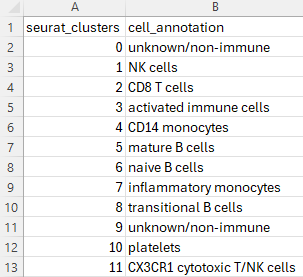
\includegraphics[width=0.45\textwidth]{Figures/annotation.png}
\caption{Example format for the required annotation file (\texttt{.csv}). The file must contain columns named \texttt{seurat\_clusters} and \texttt{cell\_annotation}; other columns are ignored.}
\label{fig:annotation_csv}
\end{figure}
\FloatBarrier

\begin{figure}[H]
\centering
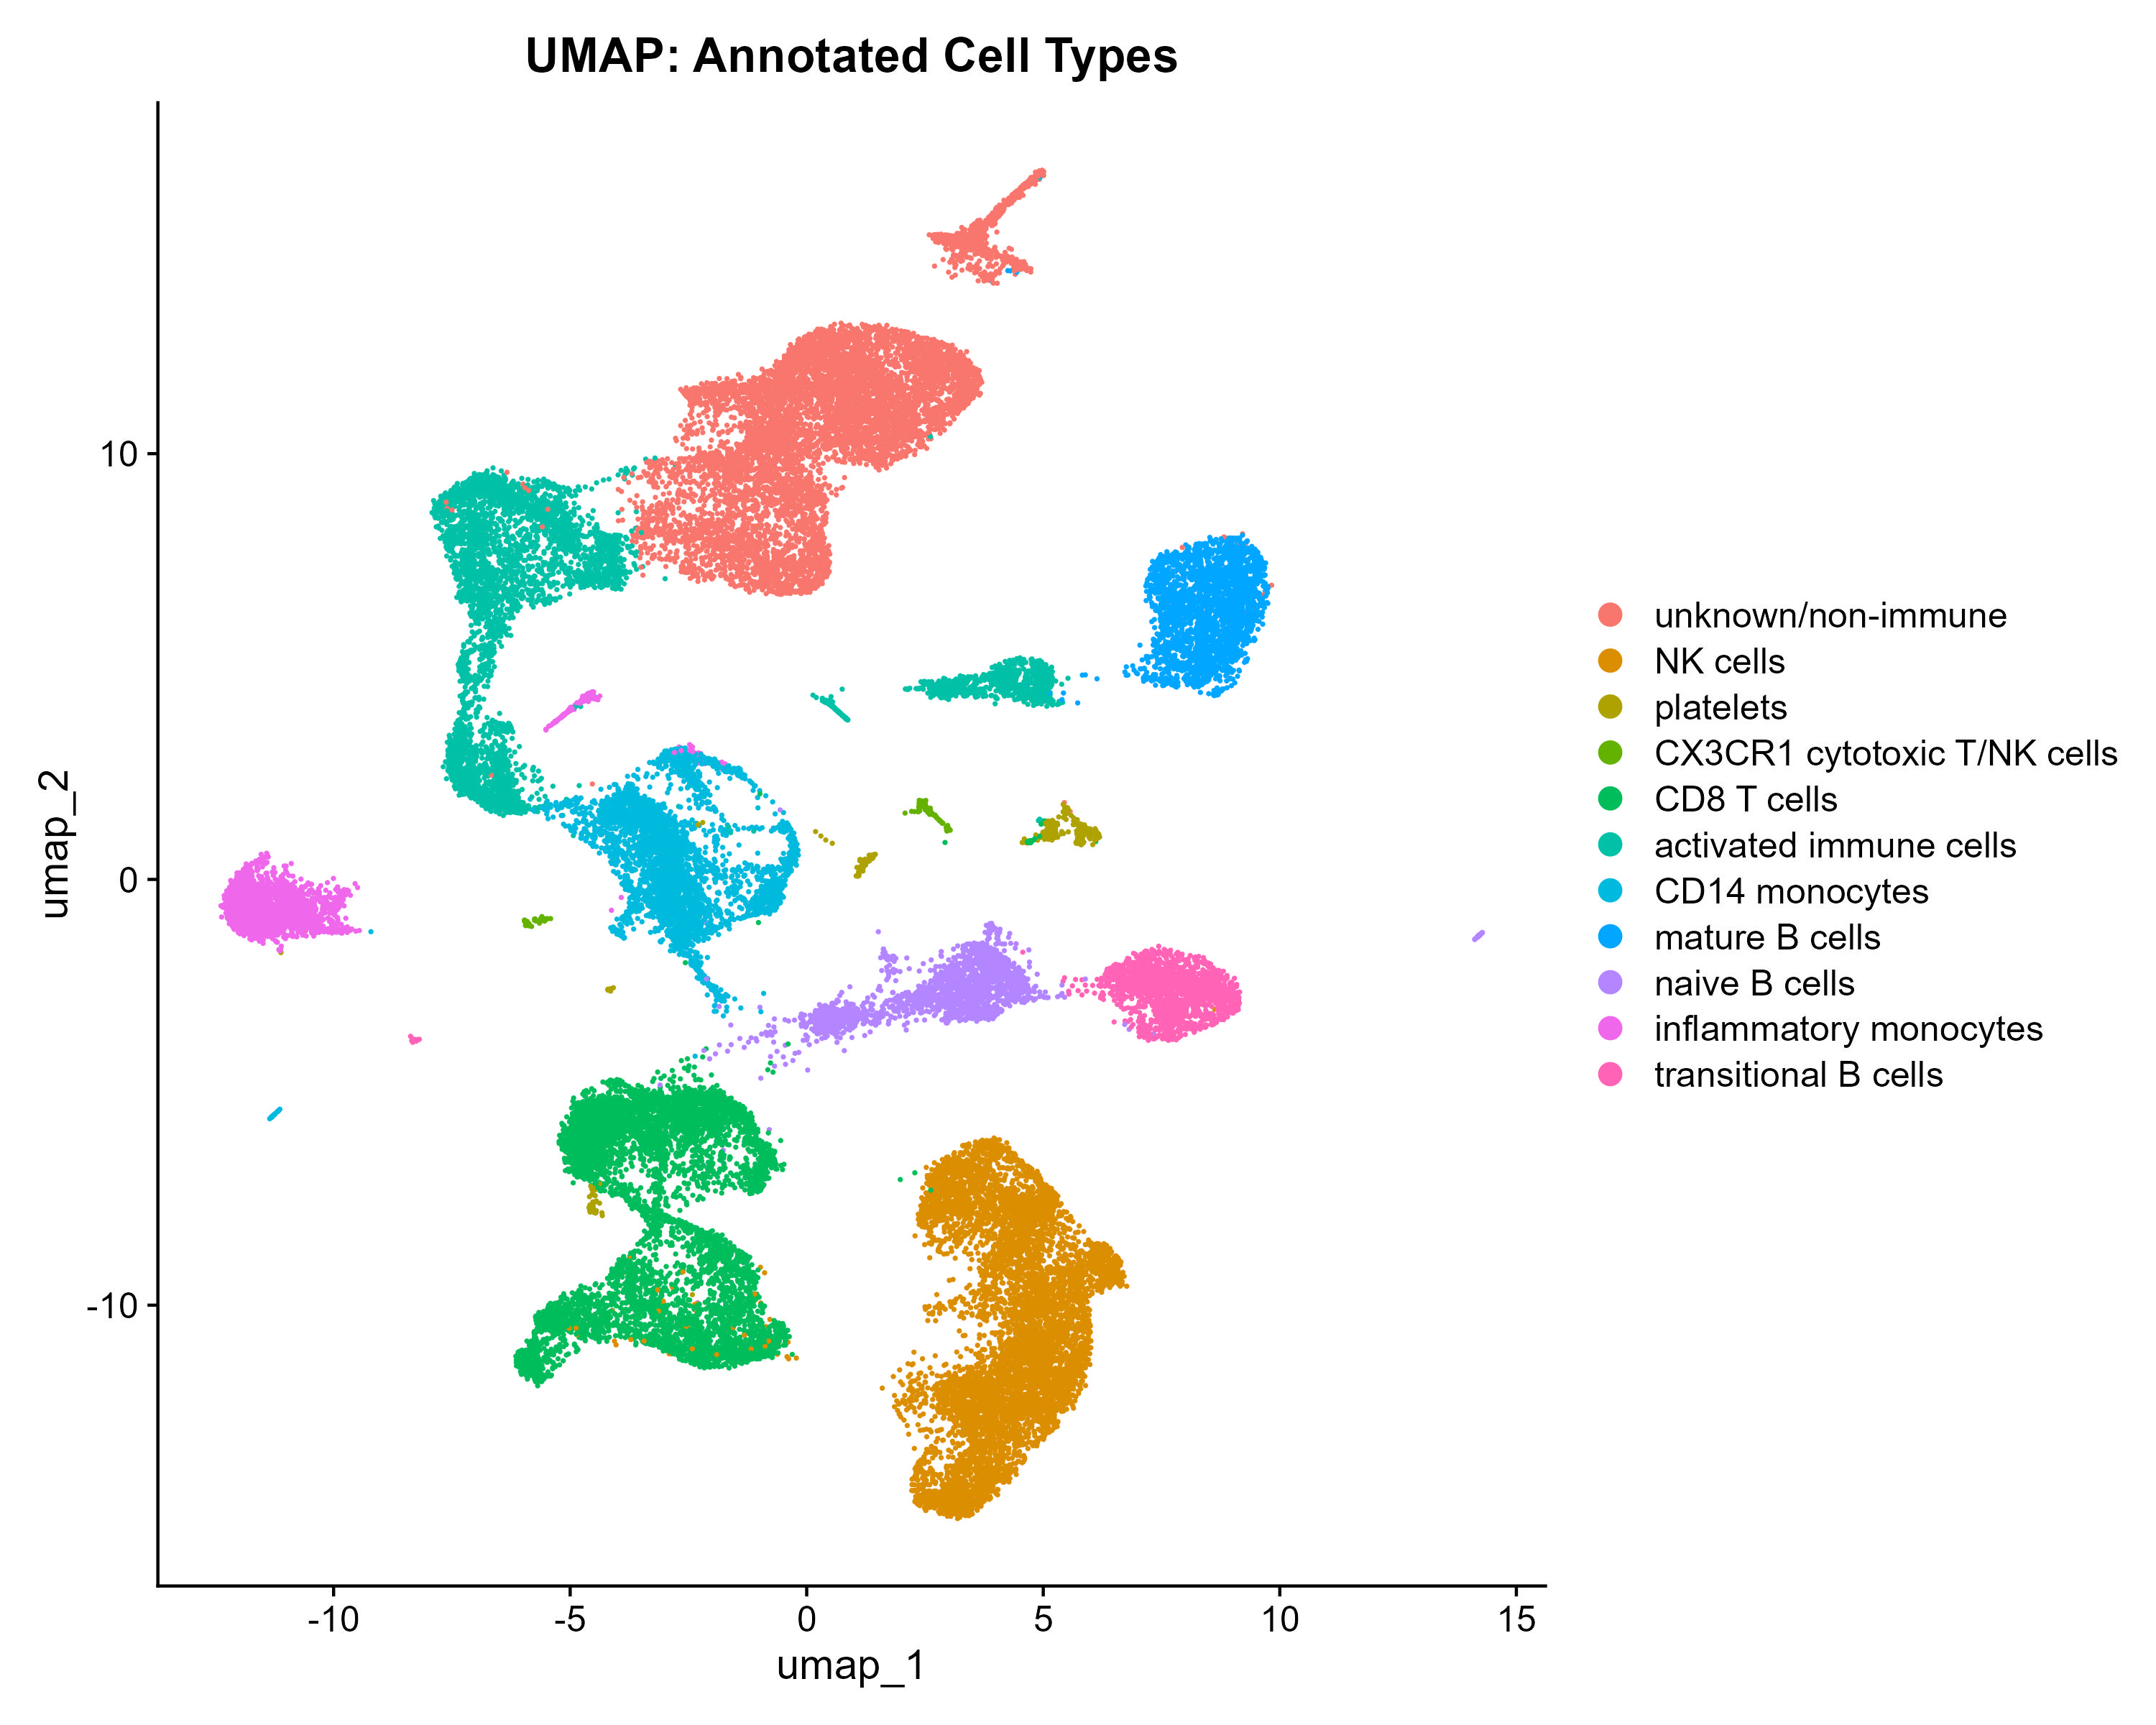
\includegraphics[width=0.5\textwidth]{Figures/umap_annotated.jpeg}
\caption{UMAP visualization with annotated cell types. Each point represents a cell and colors correspond to the user-assigned cell type labels.}
\label{fig:umap_annotated}
\end{figure}
\FloatBarrier

\begin{figure}[H]
\centering
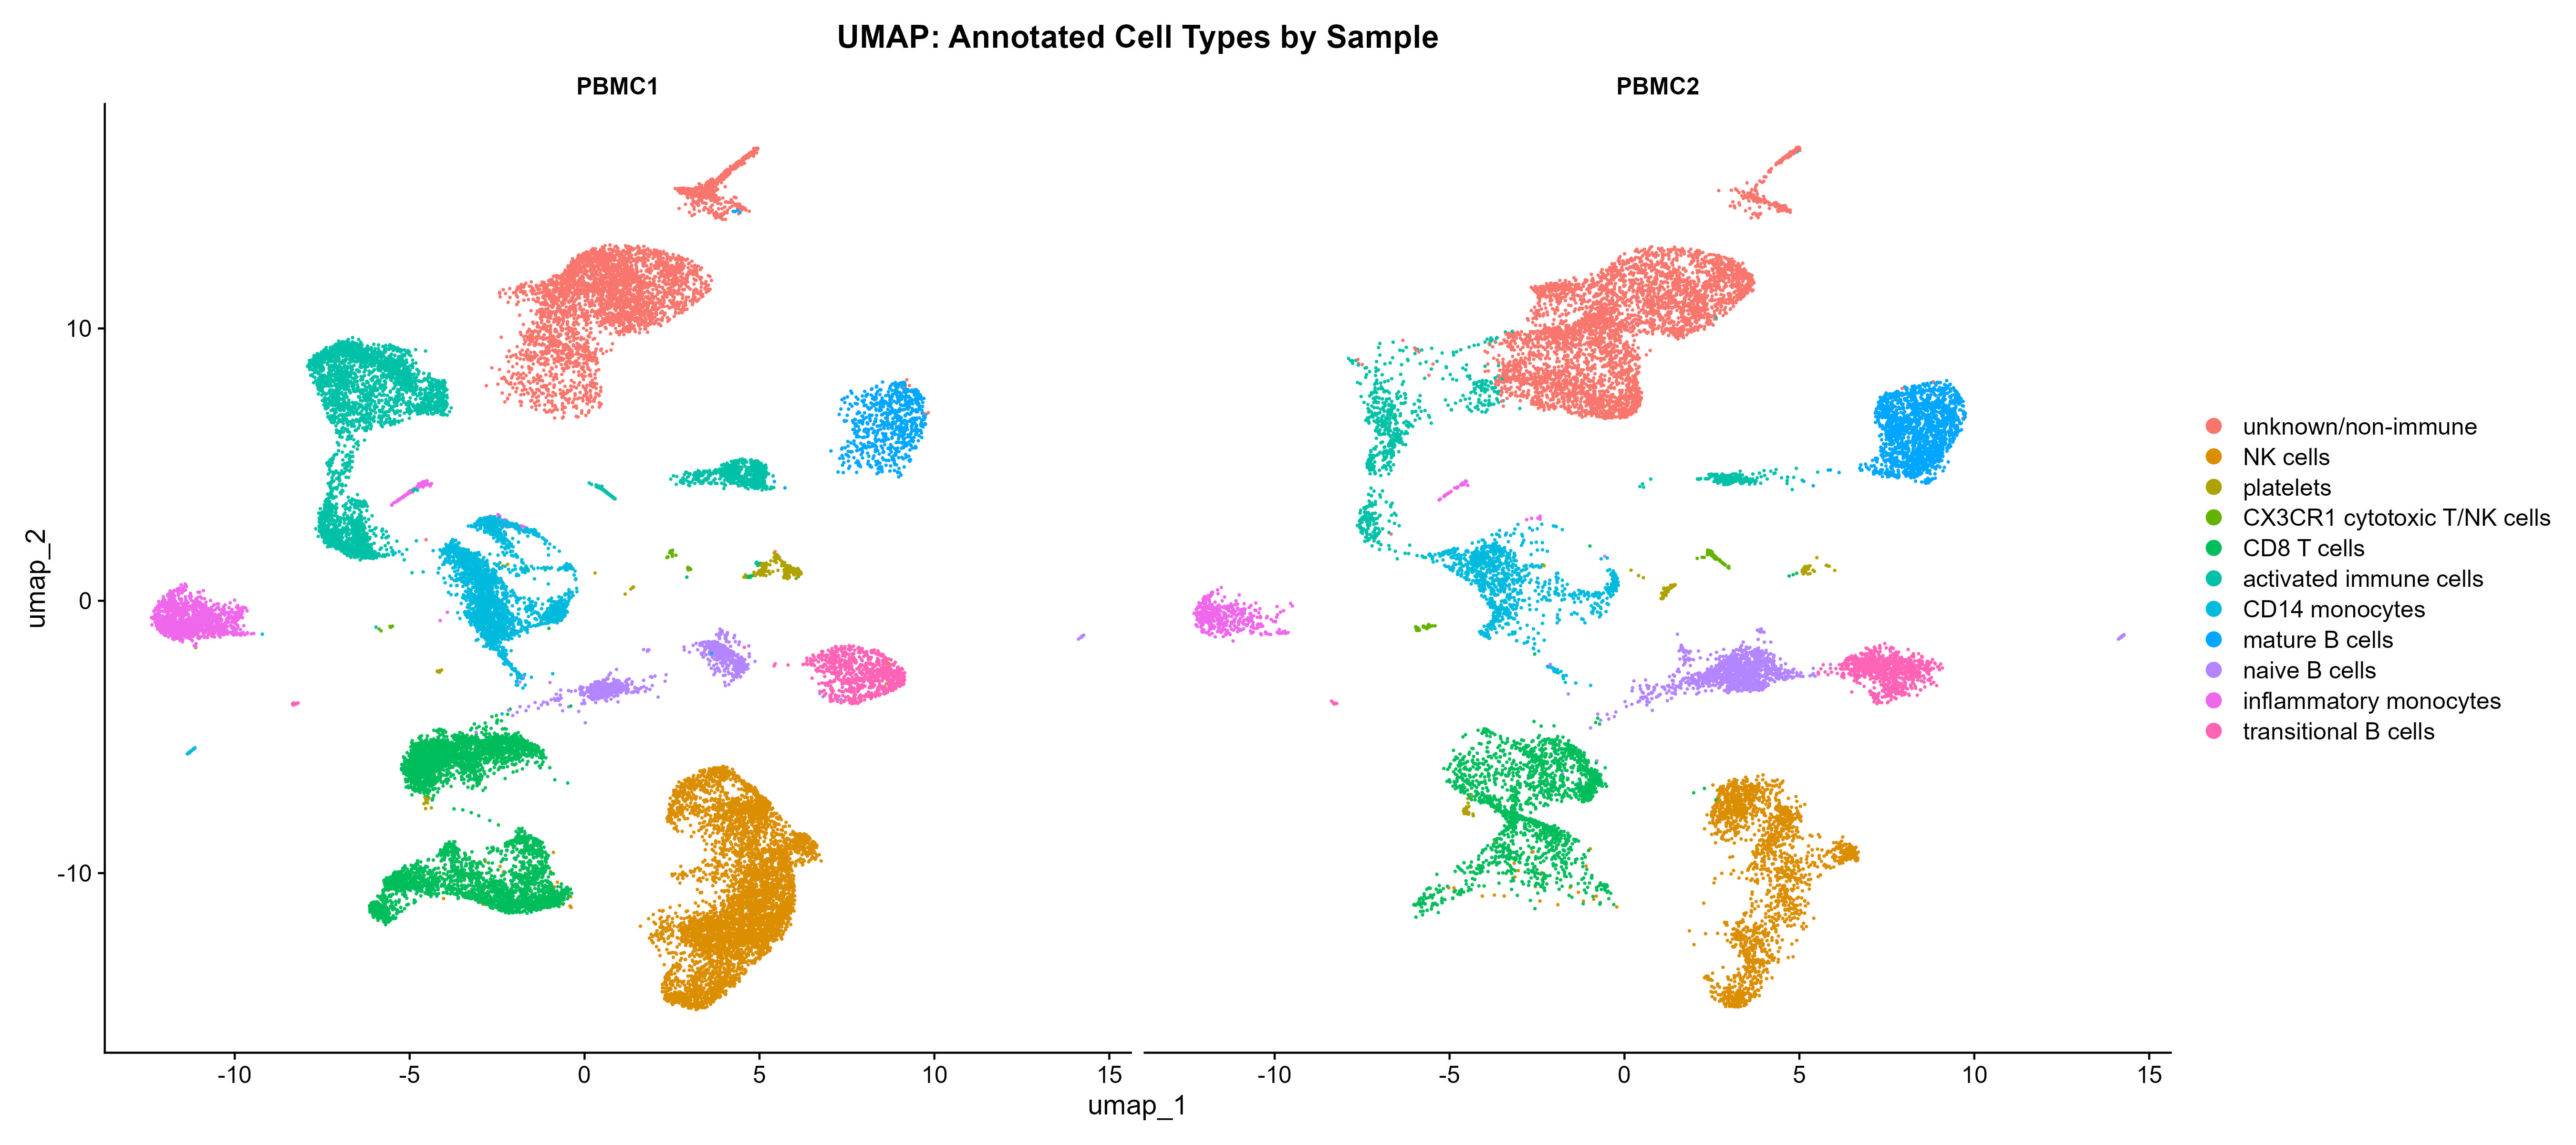
\includegraphics[width=0.8\textwidth]{Figures/umap_split_by_sample.jpeg}
\caption{Annotated UMAP split by sample. This view helps compare cell type distributions and cluster structure across different samples or conditions.}
\label{fig:umap_split_annotated}
\end{figure}
\FloatBarrier

\section{Step 9 -- Visualize gene expression (FeaturePlots)}

\textbf{Purpose.}  
This step allows users to visualize where specific genes are expressed within the dataset. Feature plots project gene expression levels onto the UMAP embedding, making it easy to see which cell populations express a gene of interest.

\textbf{What to do.}  
Enter one or more gene names (comma-separated) and generate feature plots. These plots are especially useful for confirming marker gene expression, validating cluster annotations, and exploring spatial expression patterns across cell types.

\textbf{What Cellivista does.}
\begin{itemize}[leftmargin=*,nosep]
\item Retrieves expression values for each selected gene.
\item Projects expression levels onto the UMAP embedding.
\item Generates one feature plot per gene, which can be viewed and downloaded individually or all together as a \texttt{.zip} file.
\end{itemize}

\textbf{How to interpret the plots.}
\begin{itemize}[leftmargin=*,nosep]
\item Each point represents a single cell in the UMAP space.
\item Color intensity reflects expression level, with darker colors indicating higher expression.
\item Genes that are strong markers for a cell type typically show localized expression in specific clusters.
\item Broad expression patterns may indicate shared biological functions or housekeeping roles.
\end{itemize}

\textbf{Input explained.}
\begin{itemize}
  \item \textbf{Load Seurat object from \texttt{.rds}:} Allows FeaturePlot generation from an uploaded Seurat object.
  \item \textbf{Gene list:} Enter gene symbols separated by commas, such as \texttt{ENSG00000251562-MALAT1, ENSG00000236008-AC011747\_4, ENSG00000137571-SLCO5A1, ENSG00000110013-SIAE}.
  \item \textbf{Save FeaturePlots as images:} Enables or disables export of the generated FeaturePlots.
  \item \textbf{FeaturePlot export settings:} Users can customize filename prefix, title prefix, output format, width, and height.
\end{itemize}

\textbf{Output.}
FeaturePlots for each selected gene are generated and displayed in the app. When image saving is enabled, each FeaturePlot is also made available as an individually downloadable image file.

\begin{figure}[H]
\centering

\begin{subfigure}{0.4\textwidth}
  \centering
  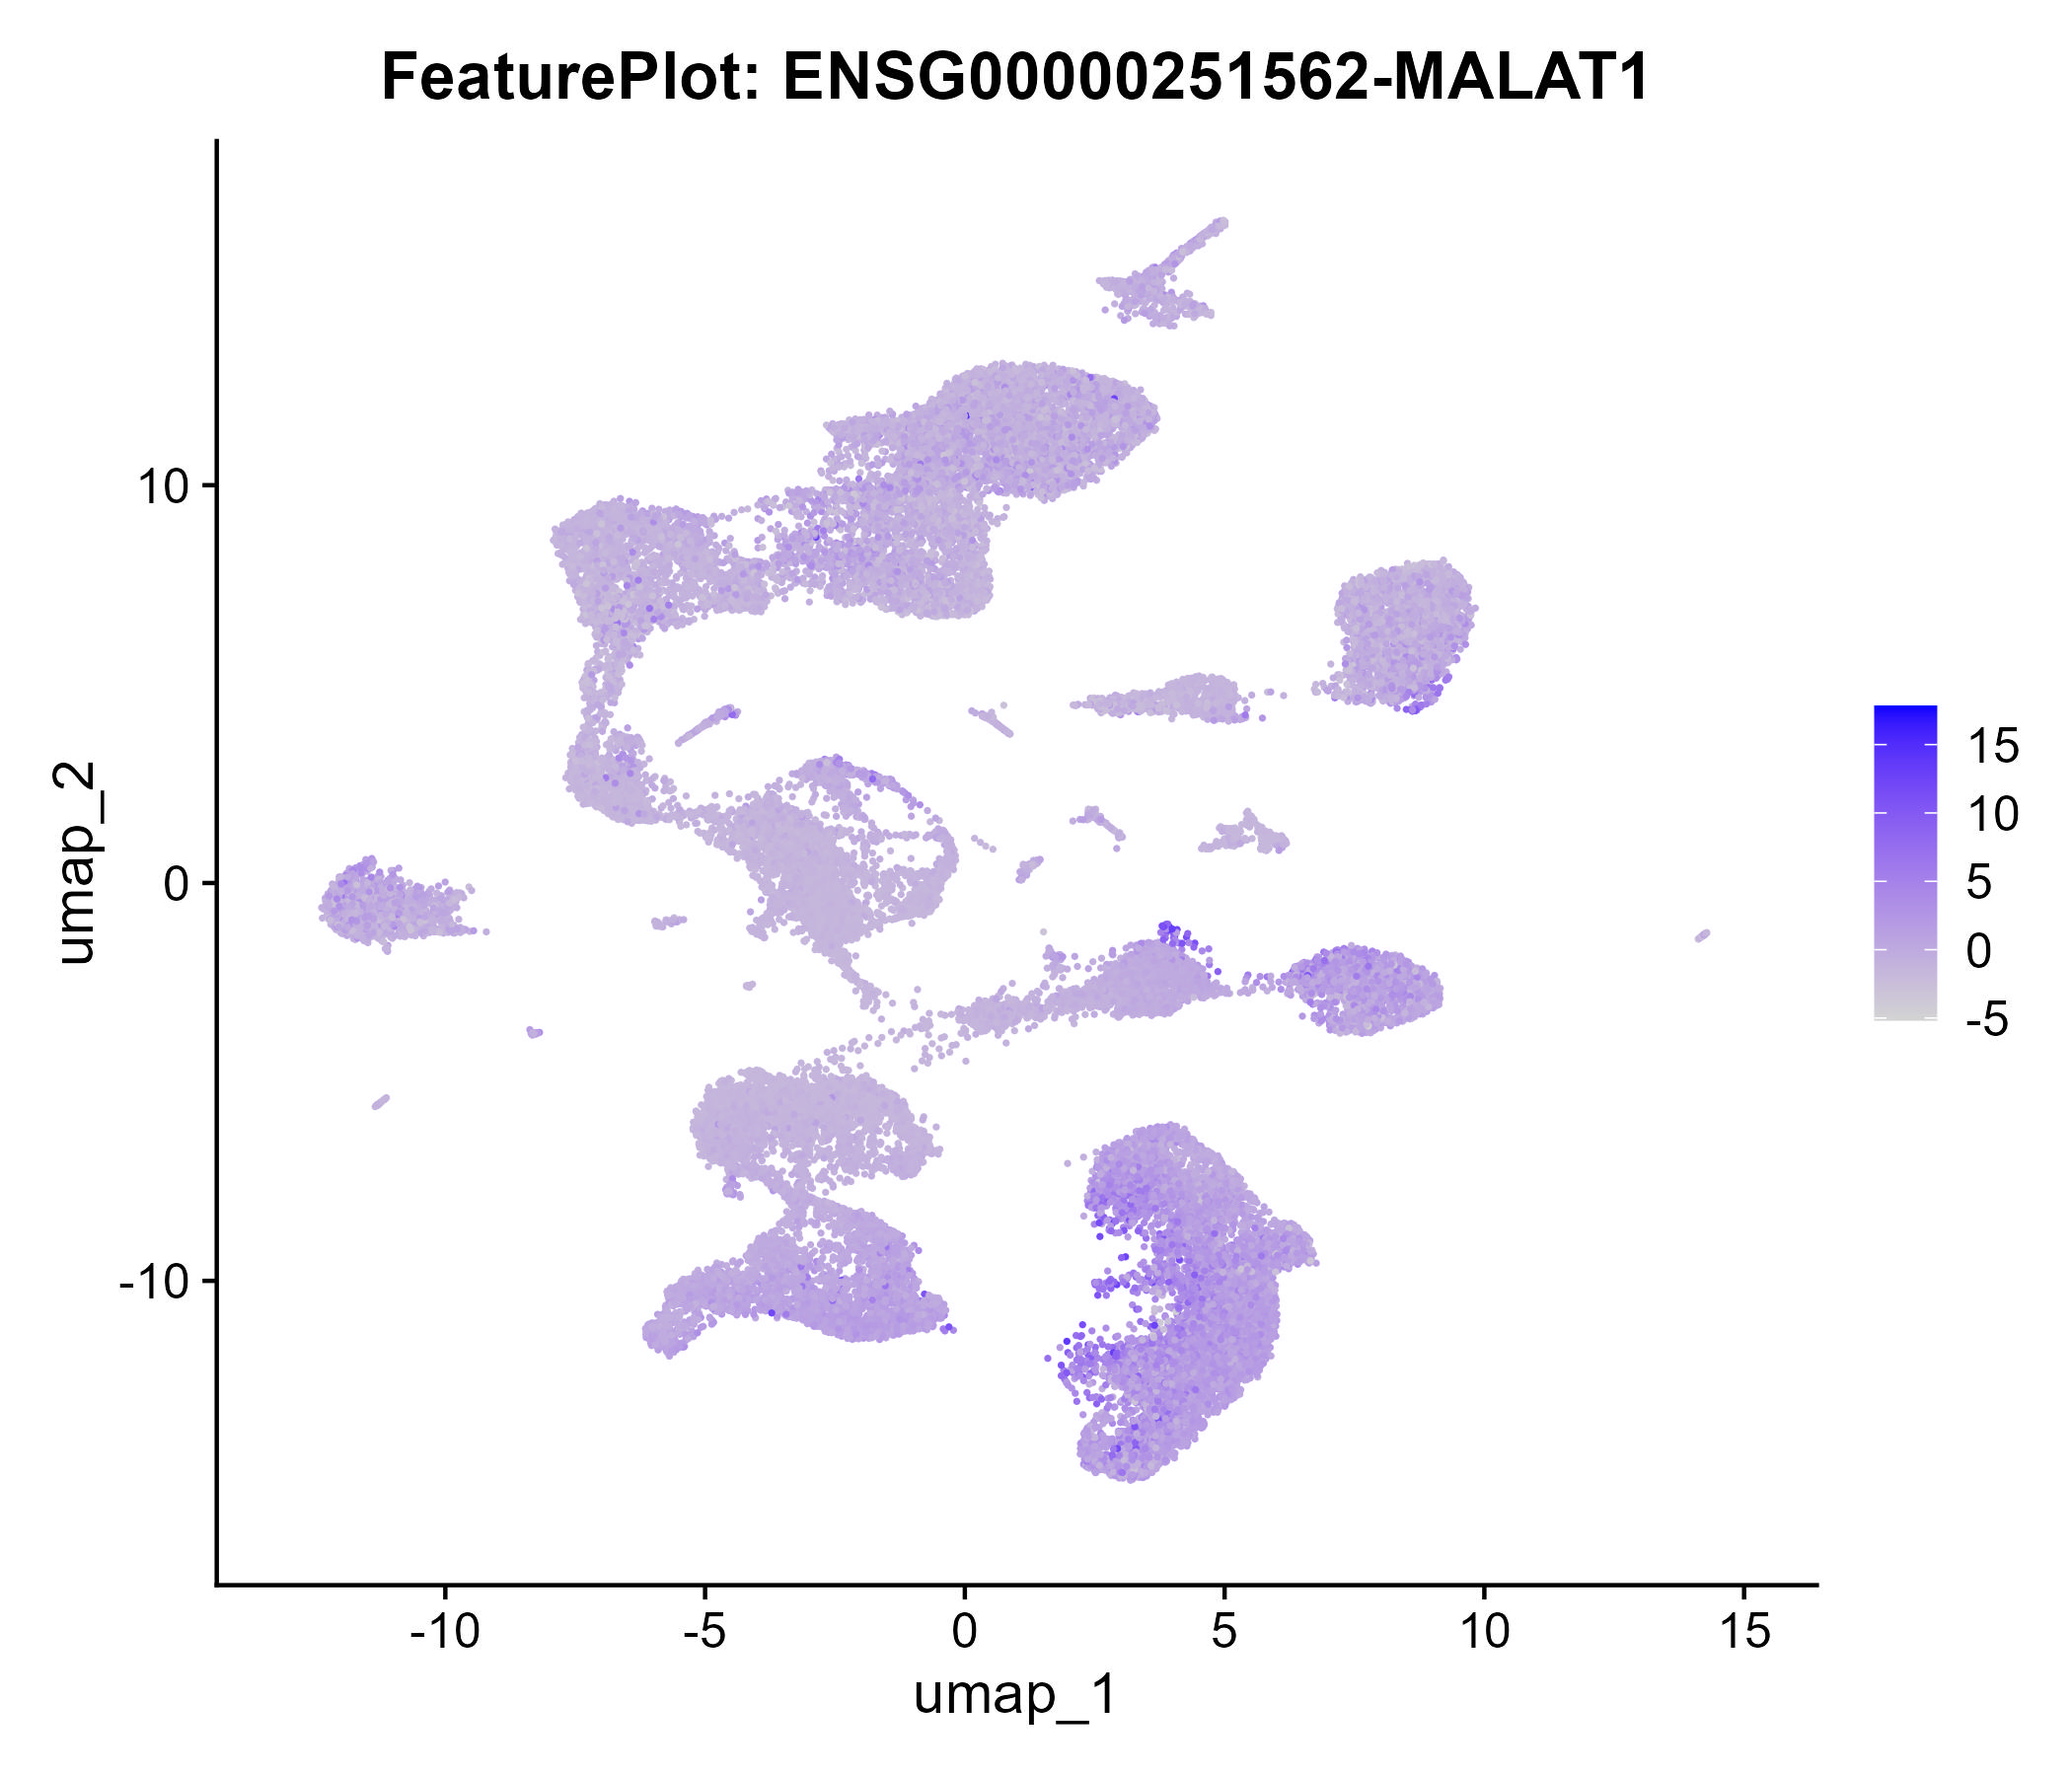
\includegraphics[width=\linewidth]{Figures/featureplot_ENSG00000251562-MALAT1.jpeg}
  \caption{\textit{MALAT1}}
\end{subfigure}
\hfill
\begin{subfigure}{0.4\textwidth}
  \centering
  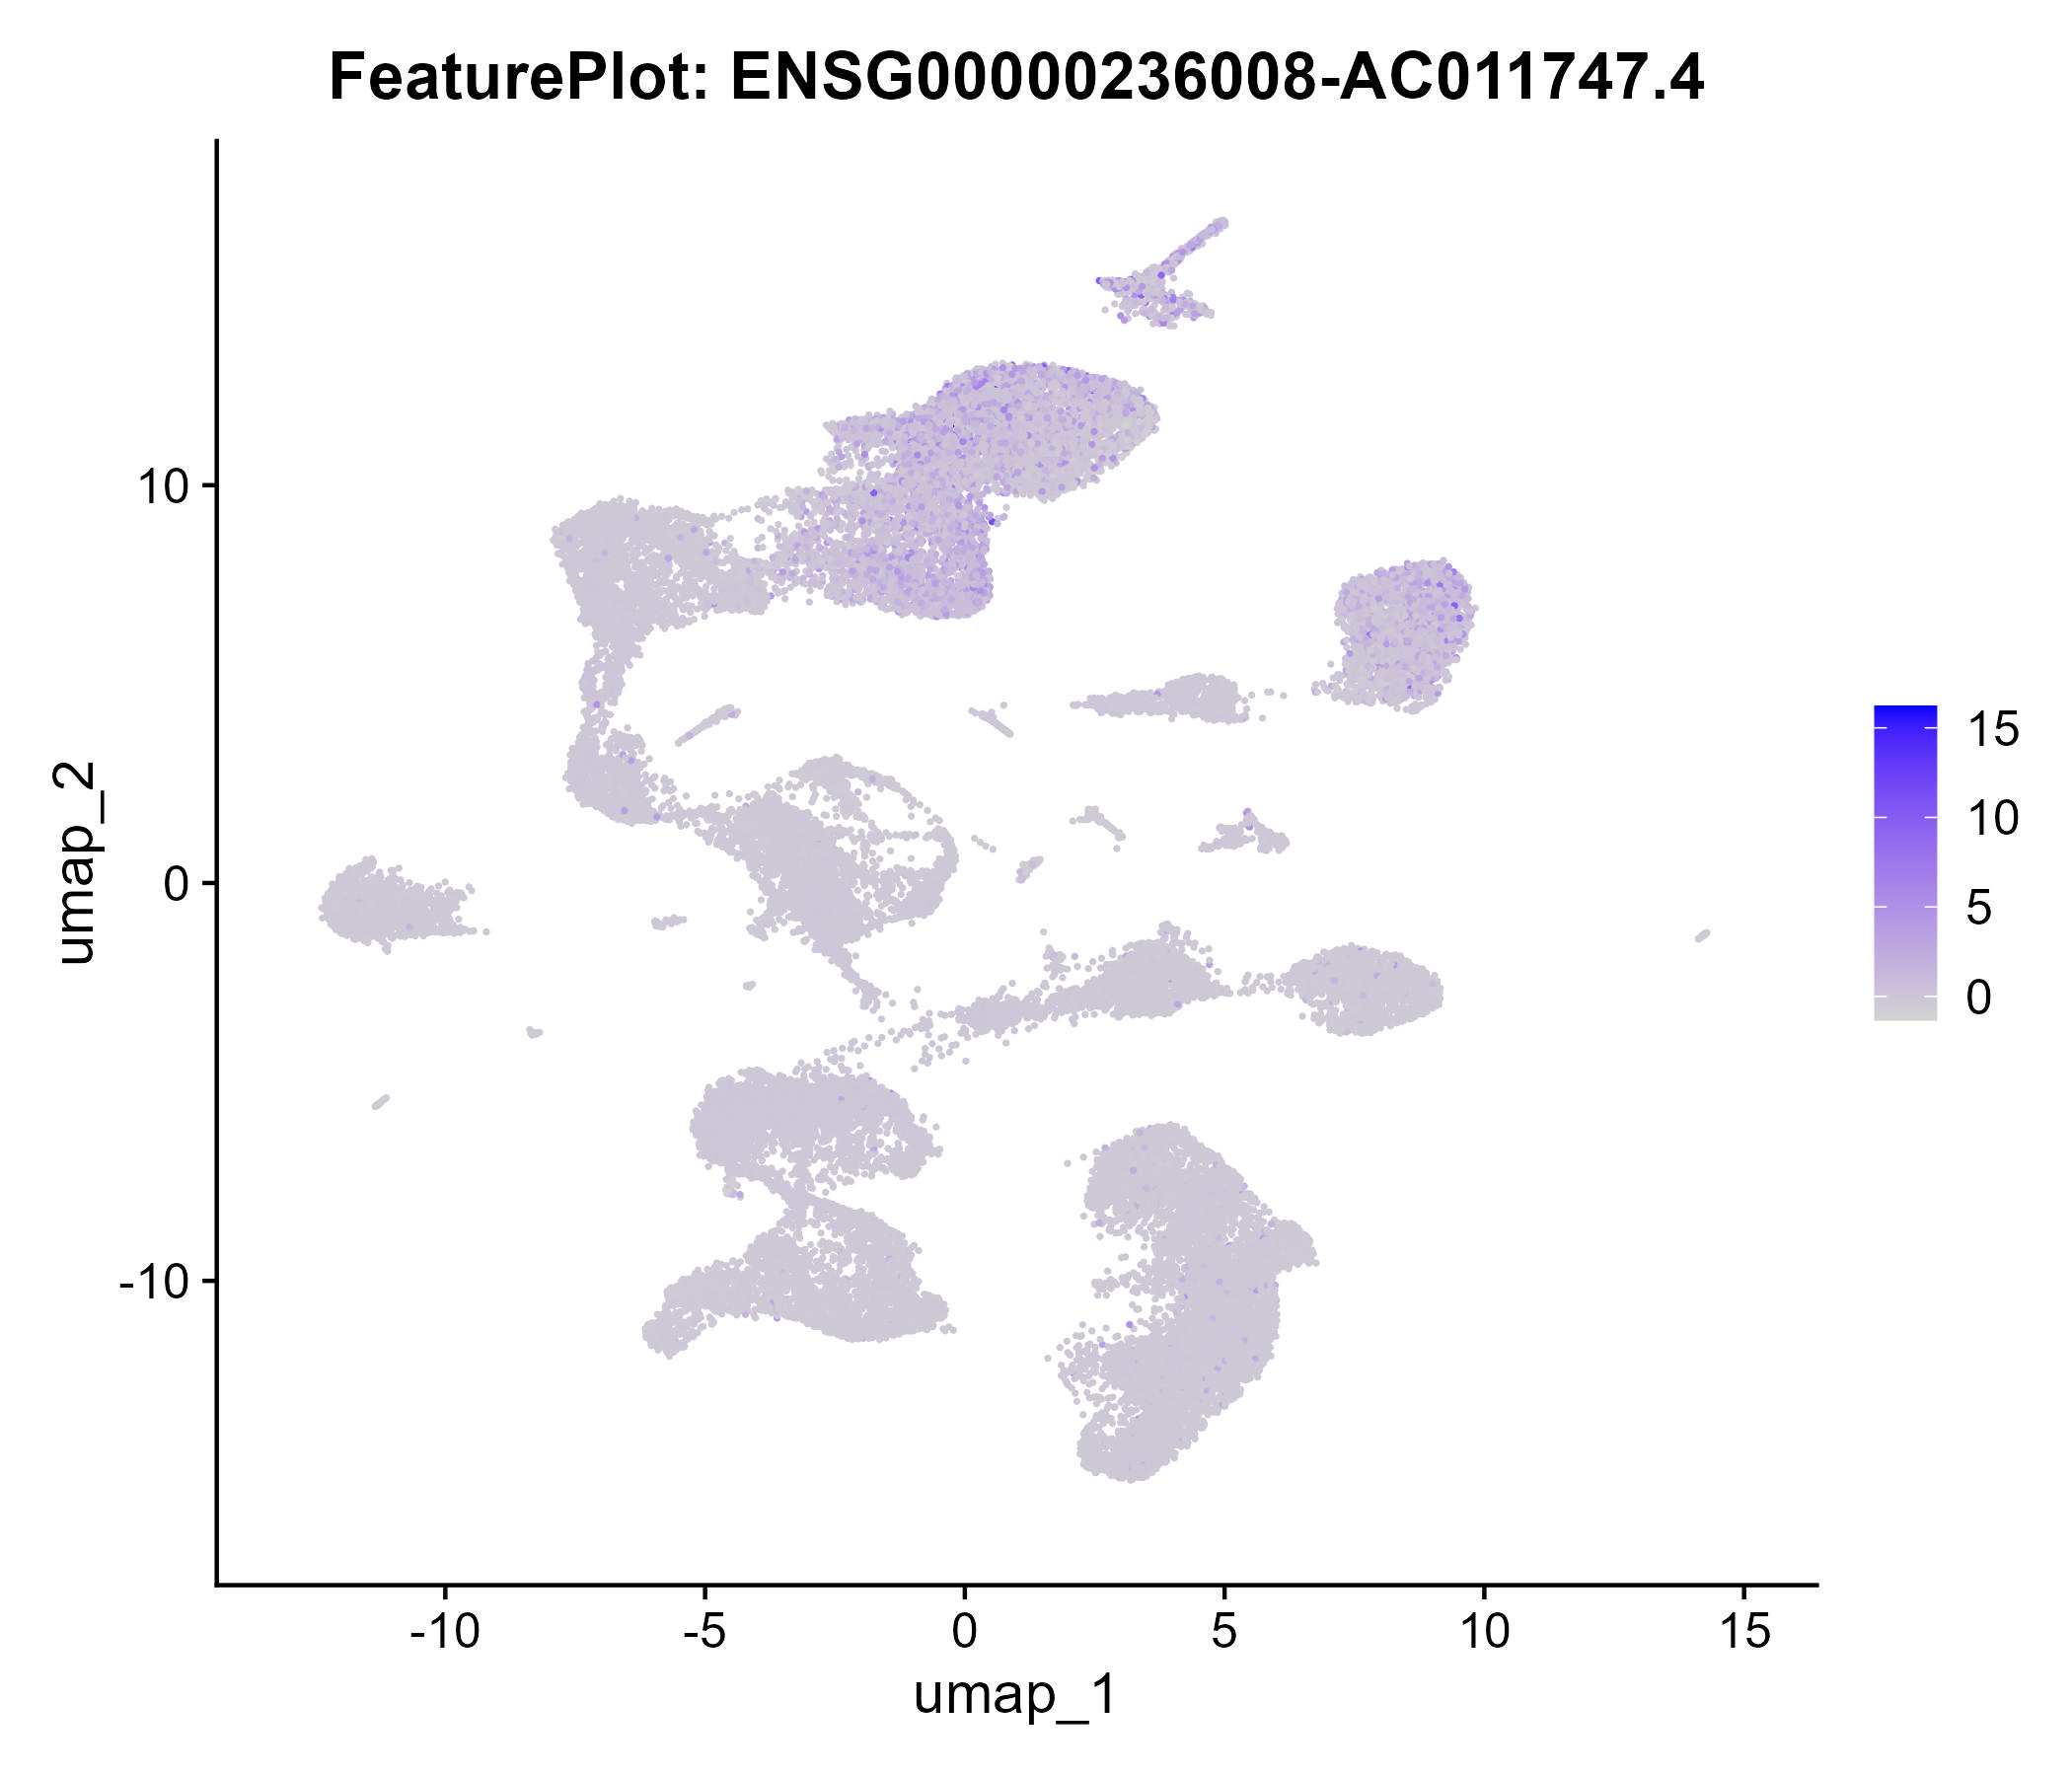
\includegraphics[width=\linewidth]{Figures/featureplot_ENSG00000236008-AC011747_4.jpeg}
  \caption{\textit{AC011747.4}}
\end{subfigure}

\vspace{0.4cm}

\begin{subfigure}{0.4\textwidth}
  \centering
  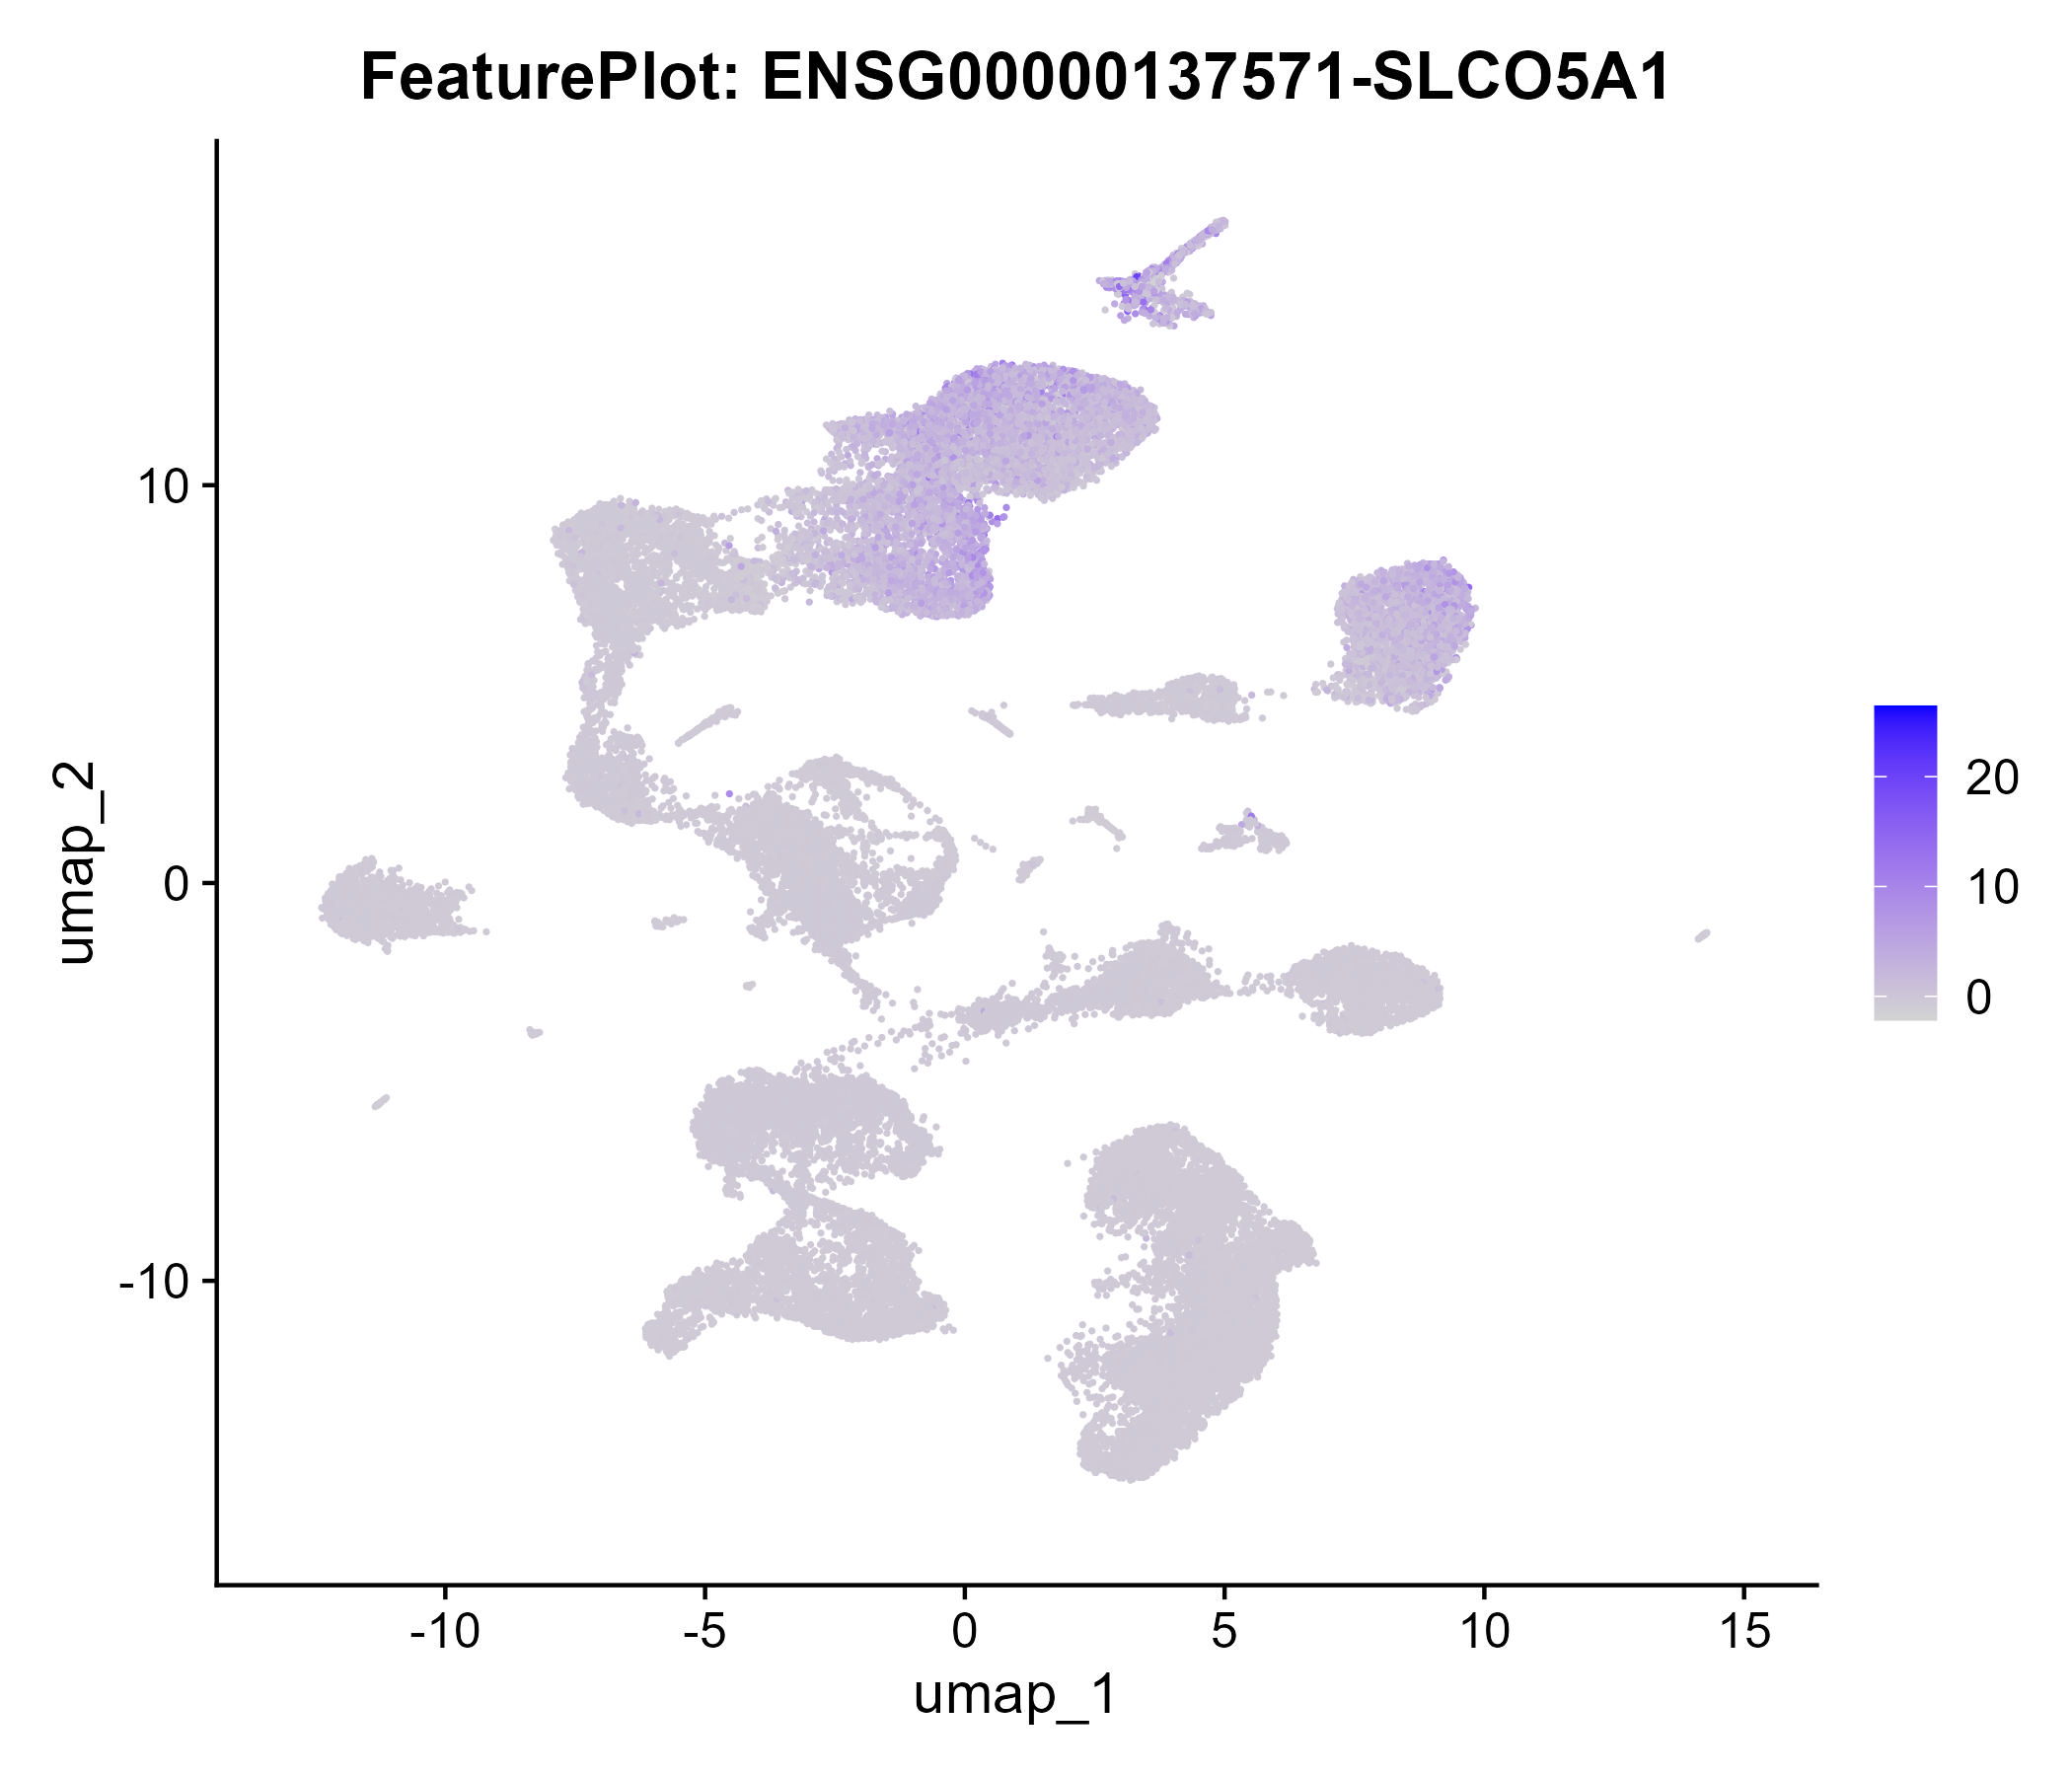
\includegraphics[width=\linewidth]{Figures/featureplot_ENSG00000137571-SLCO5A1.jpeg}
  \caption{\textit{SLCO5A1}}
\end{subfigure}
\hfill
\begin{subfigure}{0.4\textwidth}
  \centering
  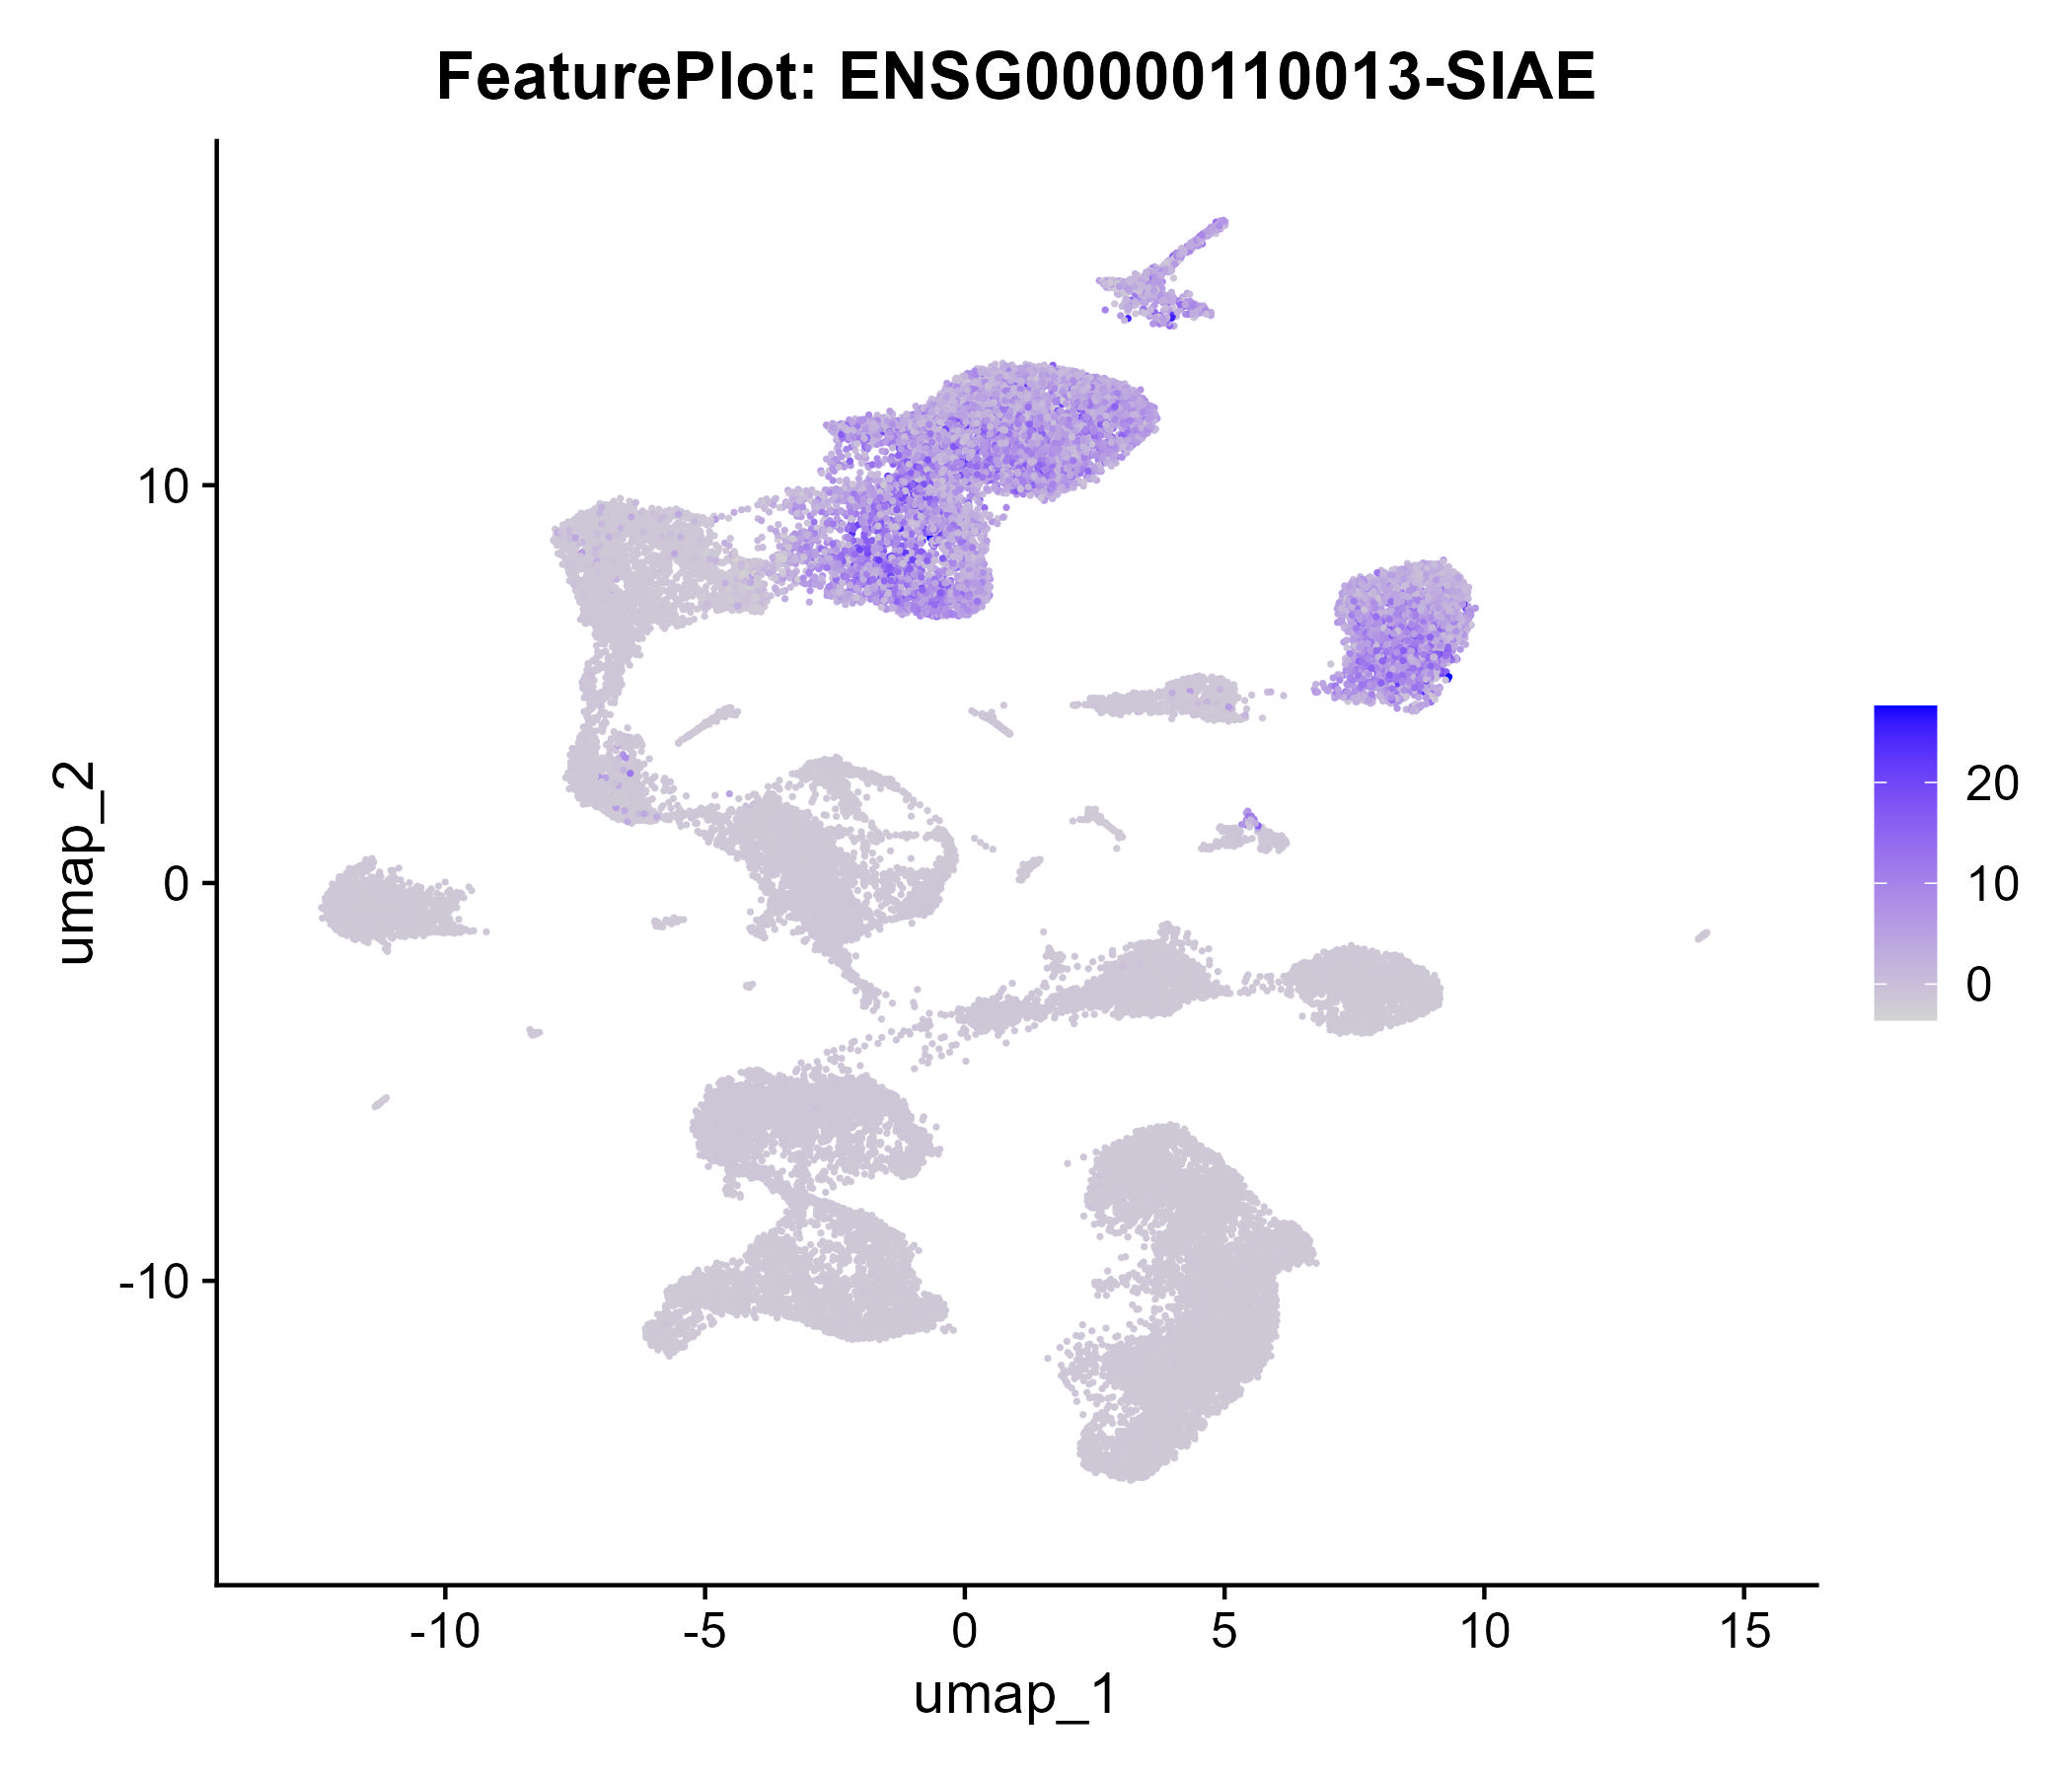
\includegraphics[width=\linewidth]{Figures/featureplot_ENSG00000110013-SIAE.jpeg}
  \caption{\textit{SIAE}}
\end{subfigure}

\caption{FeaturePlots showing expression of selected genes projected onto the UMAP embedding. Each panel illustrates a distinct expression pattern across cell populations, supporting biological interpretation and cluster validation.}
\label{fig:featureplots_2x2}
\end{figure}
\FloatBarrier

\section{Step 10 -- Visualization options}
\label{sec:viz}

\textbf{Purpose.}
This step makes three extra plots from an analyzed Seurat object: a UMAP with a chosen color palette, a heatmap of marker genes, and a bar chart of group composition per sample. Use it to prepare figures after clustering and annotation.

\textbf{What to do.}
Open the \textbf{Visualization Options} tab. By default it uses the Seurat object stored in the current session. Each of the three sections has its own controls and its own plot button, so you can run them in any order and as often as you like.

\textbf{What Cellivista does.}
\begin{itemize}
  \item Fills each \textbf{Group cells by} menu with \textbf{Active identity} and the object's categorical metadata columns that have between 1 and 200 distinct values.
  \item Picks a default grouping: \texttt{cell\_annotation} if the object has one, otherwise the cluster column (\texttt{seurat\_clusters}, or the first \texttt{*\_snn\_res.*} column), otherwise the active identity.
  \item Shows a preview of each plot in the main panel, with a short status message. The message also reports any change Cellivista made, such as a palette fallback or dropped genes.
  \item Saves the plot with the filename, format, and size you set when you click the download button under the preview.
  \item Leaves the Seurat object unchanged.
\end{itemize}

\textbf{Key options explained.}
These options apply to the whole tab or appear in every section.
\begin{itemize}
  \item \textbf{Load Seurat object from \texttt{.rds} file:} Uses an uploaded Seurat object instead of the object currently stored in the app session.
  \item \textbf{Group cells by:} The metadata column used to color or group cells. See the defaults above.
  \item \textbf{Filename:} Name of the downloaded file. Each section has its own default.
  \item \textbf{Format:} \texttt{png} (default), \texttt{pdf}, or \texttt{svg}. Exporting \texttt{svg} needs the optional \texttt{svglite} package.
  \item \textbf{Width and Height (in):} Size of the saved plot in inches, from 2 to 30. The preview is drawn at the same size.
\end{itemize}

\subsection*{UMAP palette}

\textbf{How to interpret the plot.}
Each point is a cell in the UMAP embedding, colored by the group chosen in \textbf{Group cells by}. Changing the palette changes only the colors. The positions of the cells stay the same. The object needs a UMAP, so run Step 6 first.

\textbf{Key options explained.}
\begin{itemize}
  \item \textbf{Label groups on plot:} Writes group names on the UMAP and moves them apart so they do not overlap. It is turned on by default when the default grouping is \texttt{cell\_annotation}.
  \item \textbf{Color palette:} \textbf{Default} keeps Seurat's colors. \textbf{Okabe-Ito} is a colorblind-safe palette with only 8 colors. If there are more than 8 groups, Cellivista uses viridis instead and says so in the status message. \textbf{viridis} spreads the groups along a dark-blue to yellow scale.
  \item \textbf{Export defaults:} Filename \texttt{umap\_palette}, 8 $\times$ 7 in.
\end{itemize}

\begin{figure}[H]
\centering
\begin{subfigure}[c]{0.34\textwidth}
  \centering
  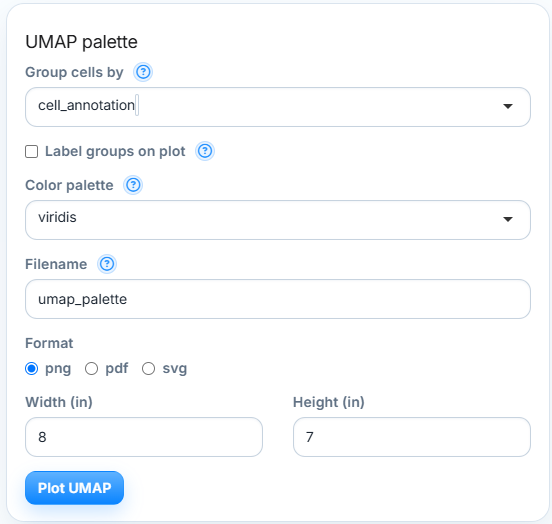
\includegraphics[width=\linewidth]{Figures/umap_palette_controls.png}
  \caption{Controls}
\end{subfigure}
\hfill
\begin{subfigure}[c]{0.62\textwidth}
  \centering
  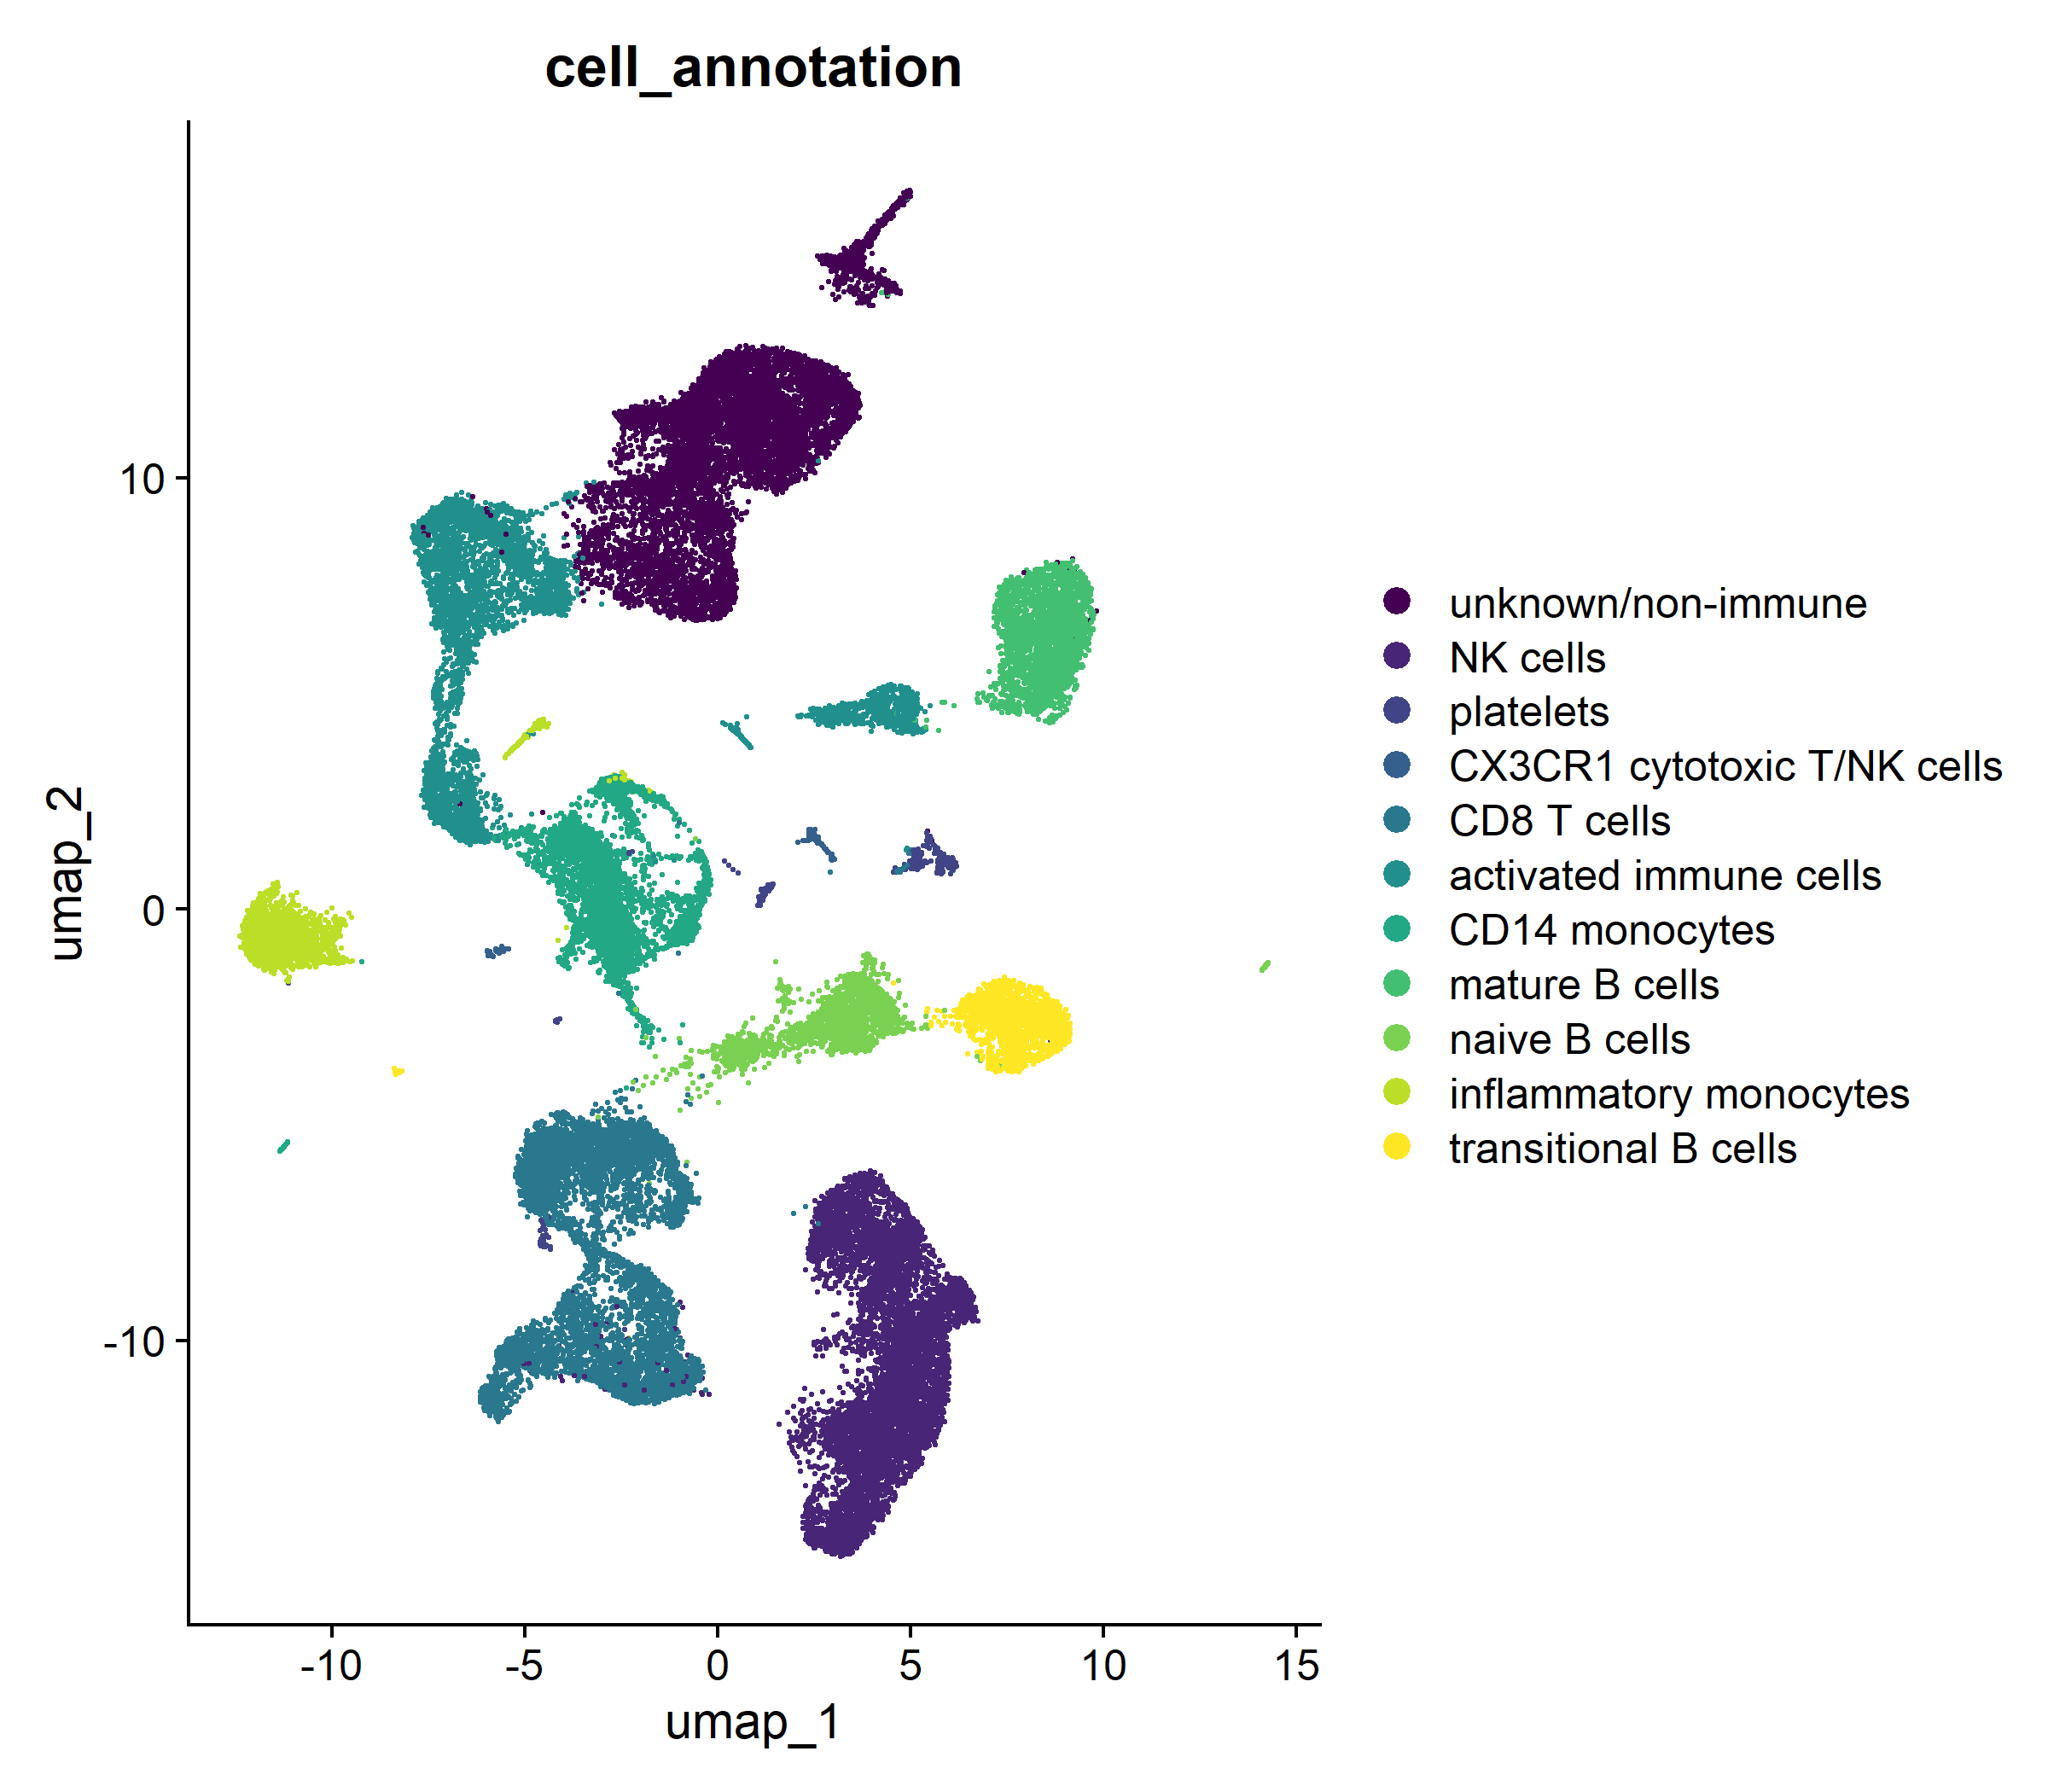
\includegraphics[width=\linewidth]{Figures/umap_palette_viridis.png}
  \caption{UMAP}
\end{subfigure}
\caption{UMAP palette section. Left: controls set to group cells by \texttt{cell\_annotation} with the viridis palette and labels off. Right: the resulting UMAP of the example data, colored by its 11 annotated cell types. Okabe-Ito is not shown, because with 11 groups it falls back to viridis.}
\label{fig:viz_umap}
\end{figure}
\FloatBarrier

\subsection*{Marker heatmap}

\textbf{How to interpret the plot.}
Rows are marker genes and columns are cells, grouped by the choice in \textbf{Group cells by}. The genes are listed cluster by cluster, so each block of rows holds the top markers of one cluster. Color shows scaled expression: yellow is higher than average for that gene and purple is lower. When the markers are specific, the bright blocks line up along a diagonal.

\textbf{Key options explained.}
\begin{itemize}
  \item \textbf{Upload marker table:} Optional. Upload \texttt{all\_marker.csv} or \texttt{top15\_marker.csv} from Step 7. If you upload nothing, Cellivista uses the markers from the Cluster-wise DGEA run in the current session. If neither is available, it stops and asks you to run Step 7 or upload a table.
  \item \textbf{Group cells by:} Groups the heatmap columns. If one cluster maps to more than one value of the chosen column, Cellivista groups by cluster instead and says so.
  \item \textbf{Top genes per cluster:} 3, 5, 10, or 15 positive markers per cluster, ranked by \texttt{avg\_log2FC}. The default is 5. \texttt{top15\_marker.csv} has no \texttt{avg\_log2FC} column, so its file order is kept and at most 15 genes per cluster are available. If a cluster has fewer genes than requested, the status message says so.
  \item \textbf{Cells per cluster:} The maximum number of cells drawn per cluster. The default is 200, and the allowed range is 10 to 5000. Cells are sampled with a fixed seed, so the same settings give the same plot. Lower values use less memory on large datasets.
  \item \textbf{Export defaults:} Filename \texttt{marker\_heatmap}, 18 $\times$ 12 in.
\end{itemize}

\textbf{Checks on the marker table.}
Cellivista uses the \texttt{SCT} assay when the object has one. It drops clusters and genes from the table that are not in the object, and reports both. It stops with an error if no cluster matches, or if fewer than half of the selected genes are found. That usually means the table came from a different object, so run Step 7 again on the current one.

\begin{figure}[H]
\centering
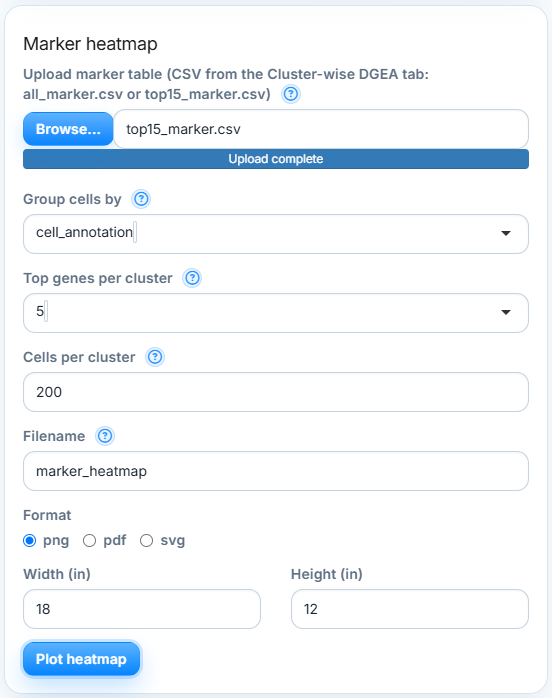
\includegraphics[width=0.4\textwidth]{Figures/heatmap_controls.png}
\caption{Marker heatmap controls, with \texttt{top15\_marker.csv} uploaded, cells grouped by \texttt{cell\_annotation}, the top 5 genes per cluster, 200 cells per cluster, and the default 18 $\times$ 12 in export size.}
\label{fig:viz_heatmap_controls}
\end{figure}

\begin{figure}[H]
\centering
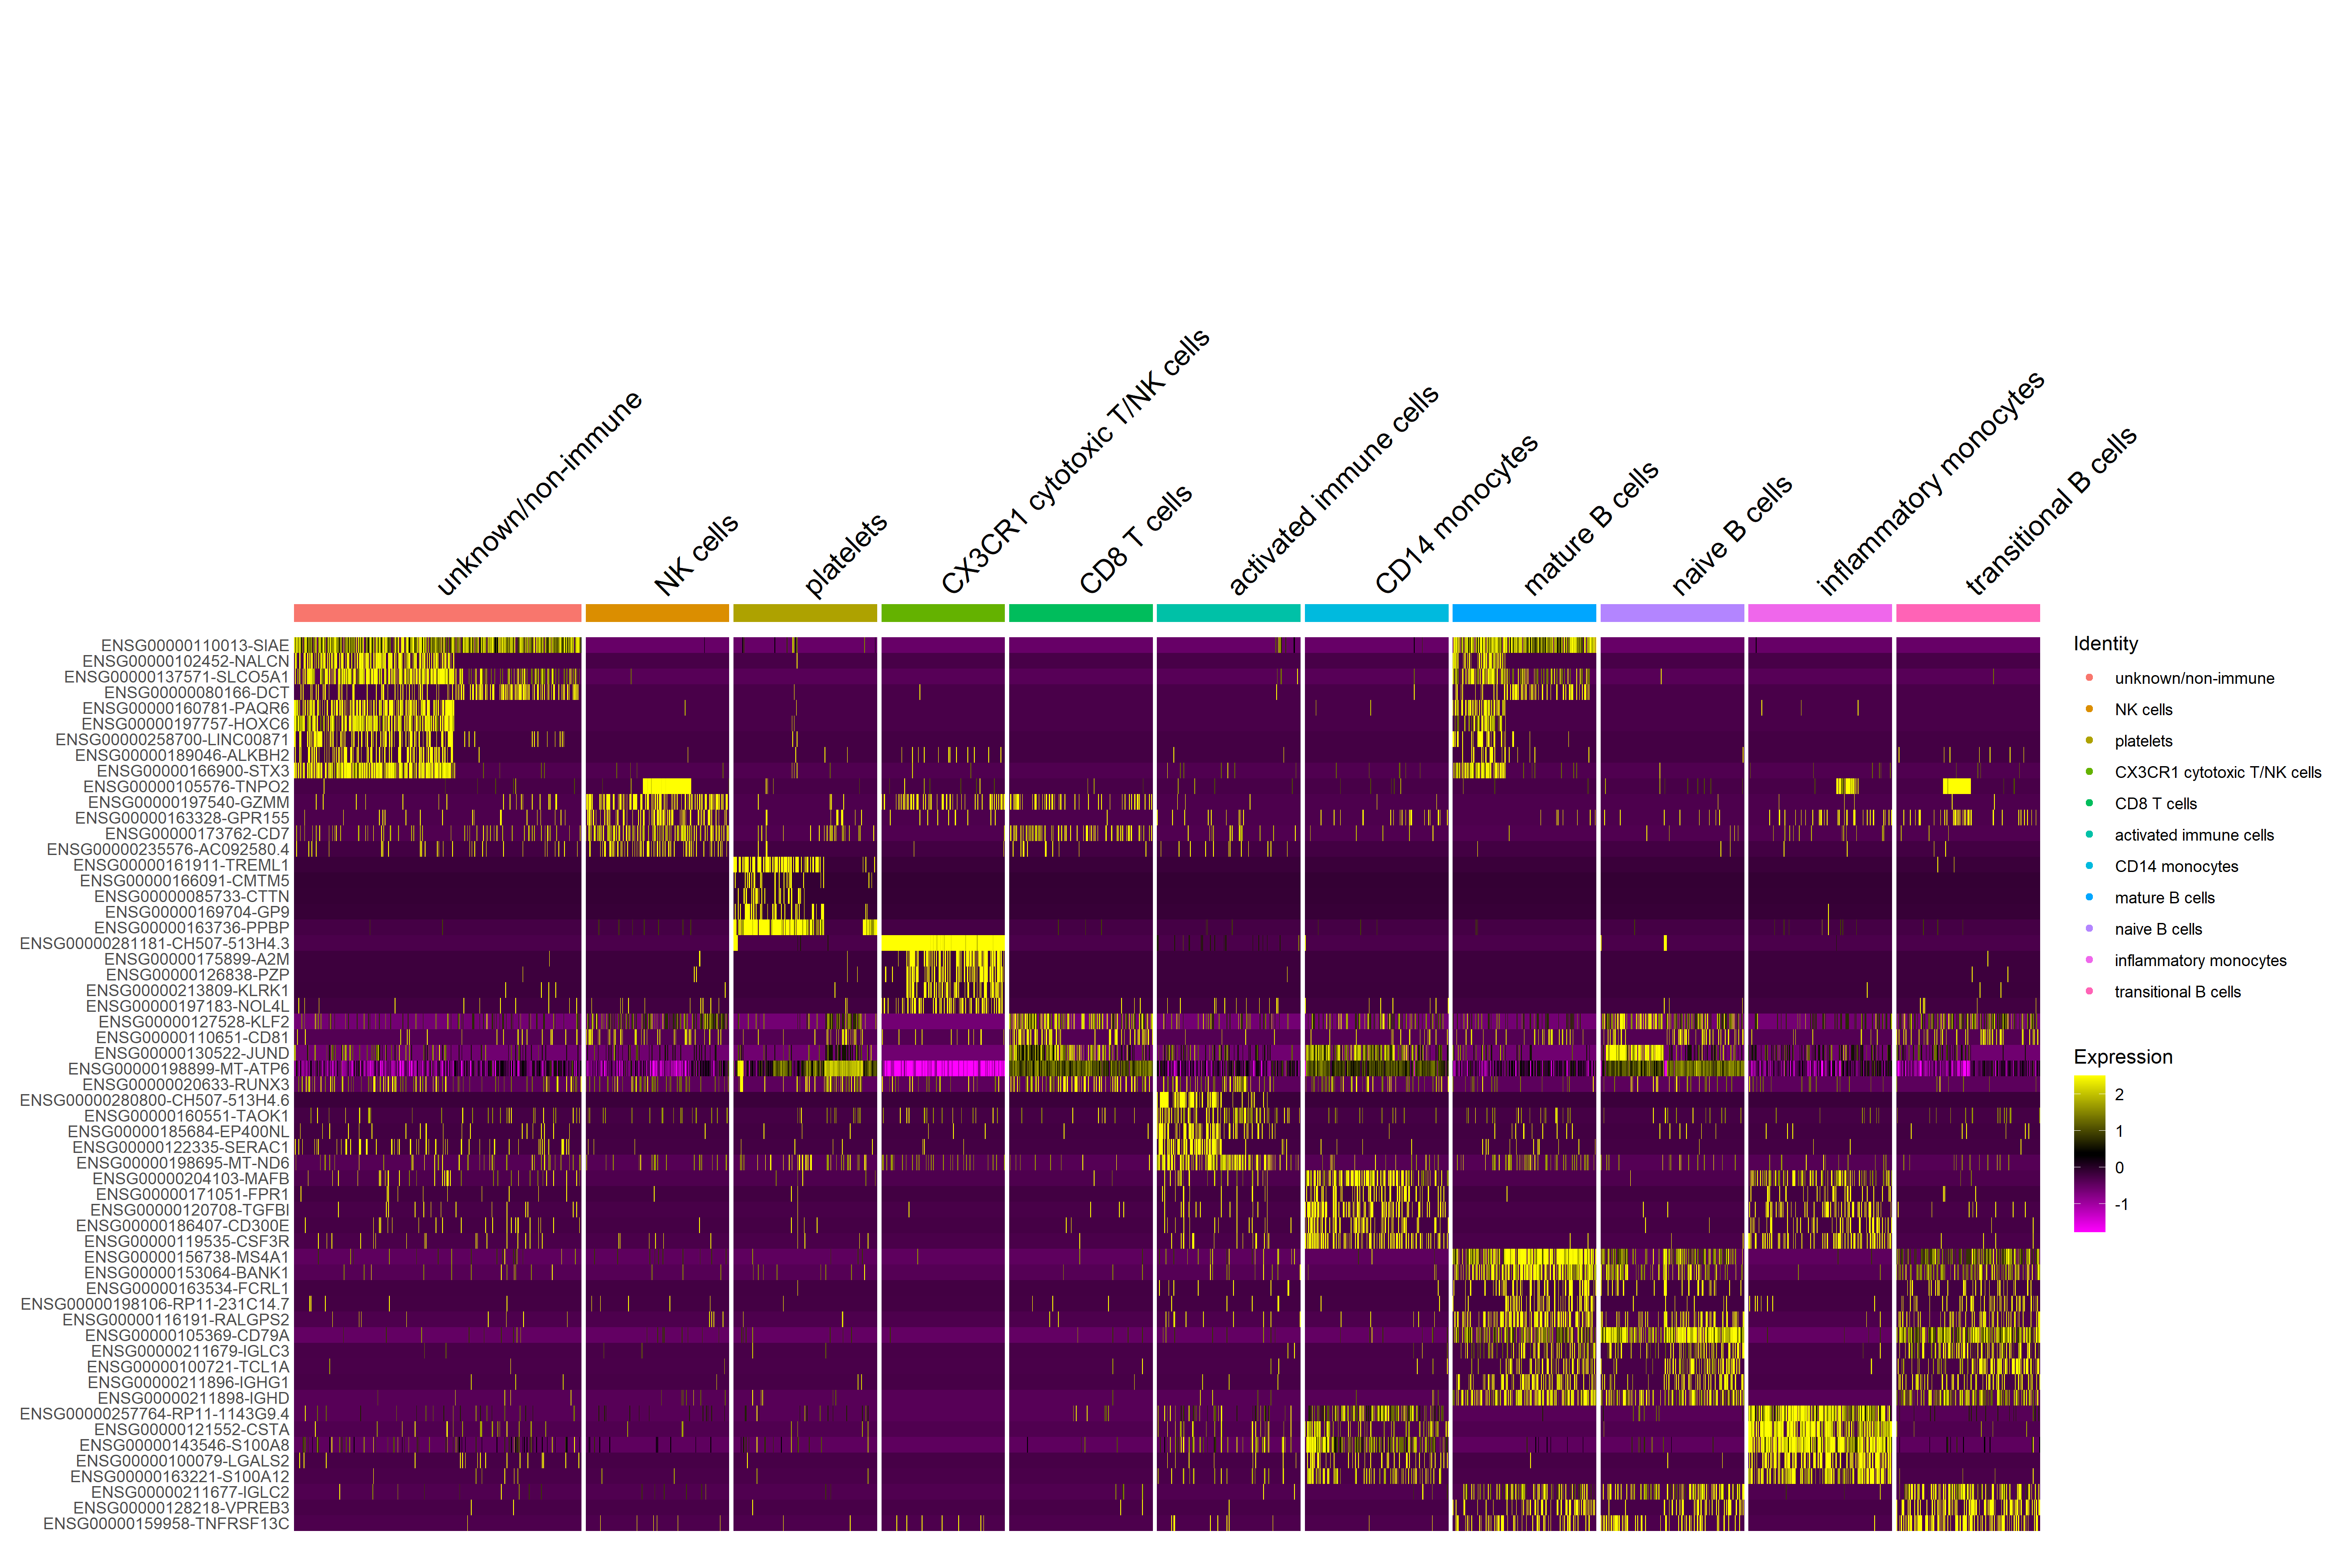
\includegraphics[width=\textwidth,trim=0 0 0 0.3\textwidth,clip]{Figures/marker_heatmap_top5.png}
\caption{Marker heatmap of the example data: the top 5 markers for each of the 11 annotated cell types, with up to 200 cells per cluster. The blank margin above the group labels is cropped in this figure.}
\label{fig:viz_heatmap}
\end{figure}
\FloatBarrier

\subsection*{Cluster composition}

\textbf{How to interpret the plot.}
Each bar adds up to 100\%. With \textbf{Bars} set to \texttt{samples}, there is one bar per sample, split into the groups chosen in \textbf{Group cells by}. Compare the bars to see whether a cell type is more common in one sample than in another. With \texttt{groups}, there is one bar per group, split by sample, which shows how much each sample contributes to that group. The bars show proportions, not cell counts.

\textbf{Key options explained.}
\begin{itemize}
  \item \textbf{Bars:} \texttt{samples} (default) draws one bar per sample, filled by group. \texttt{groups} draws one bar per group, filled by sample.
  \item \textbf{Export defaults:} Filename \texttt{cluster\_composition}, 8 $\times$ 6 in.
\end{itemize}

Samples come from the \texttt{SampleLabel} column. If the object has no usable \texttt{SampleLabel} column, Cellivista draws a single ``All cells'' bar and says so. Cells with a blank sample label are shown as ``Unlabeled''.

\begin{figure}[H]
\centering
\begin{subfigure}[c]{0.34\textwidth}
  \centering
  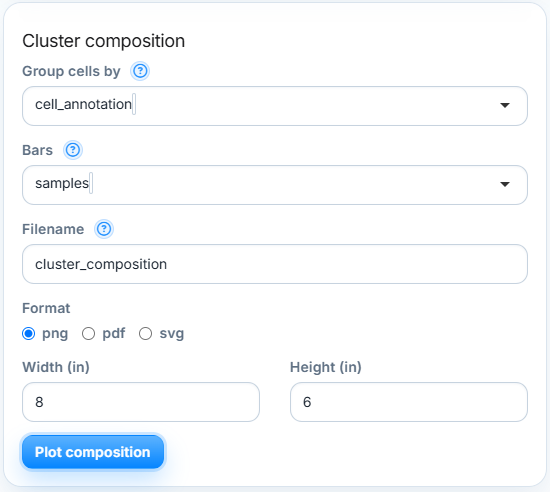
\includegraphics[width=\linewidth]{Figures/composition_controls.png}
  \caption{Controls}
\end{subfigure}
\hfill
\begin{subfigure}[c]{0.62\textwidth}
  \centering
  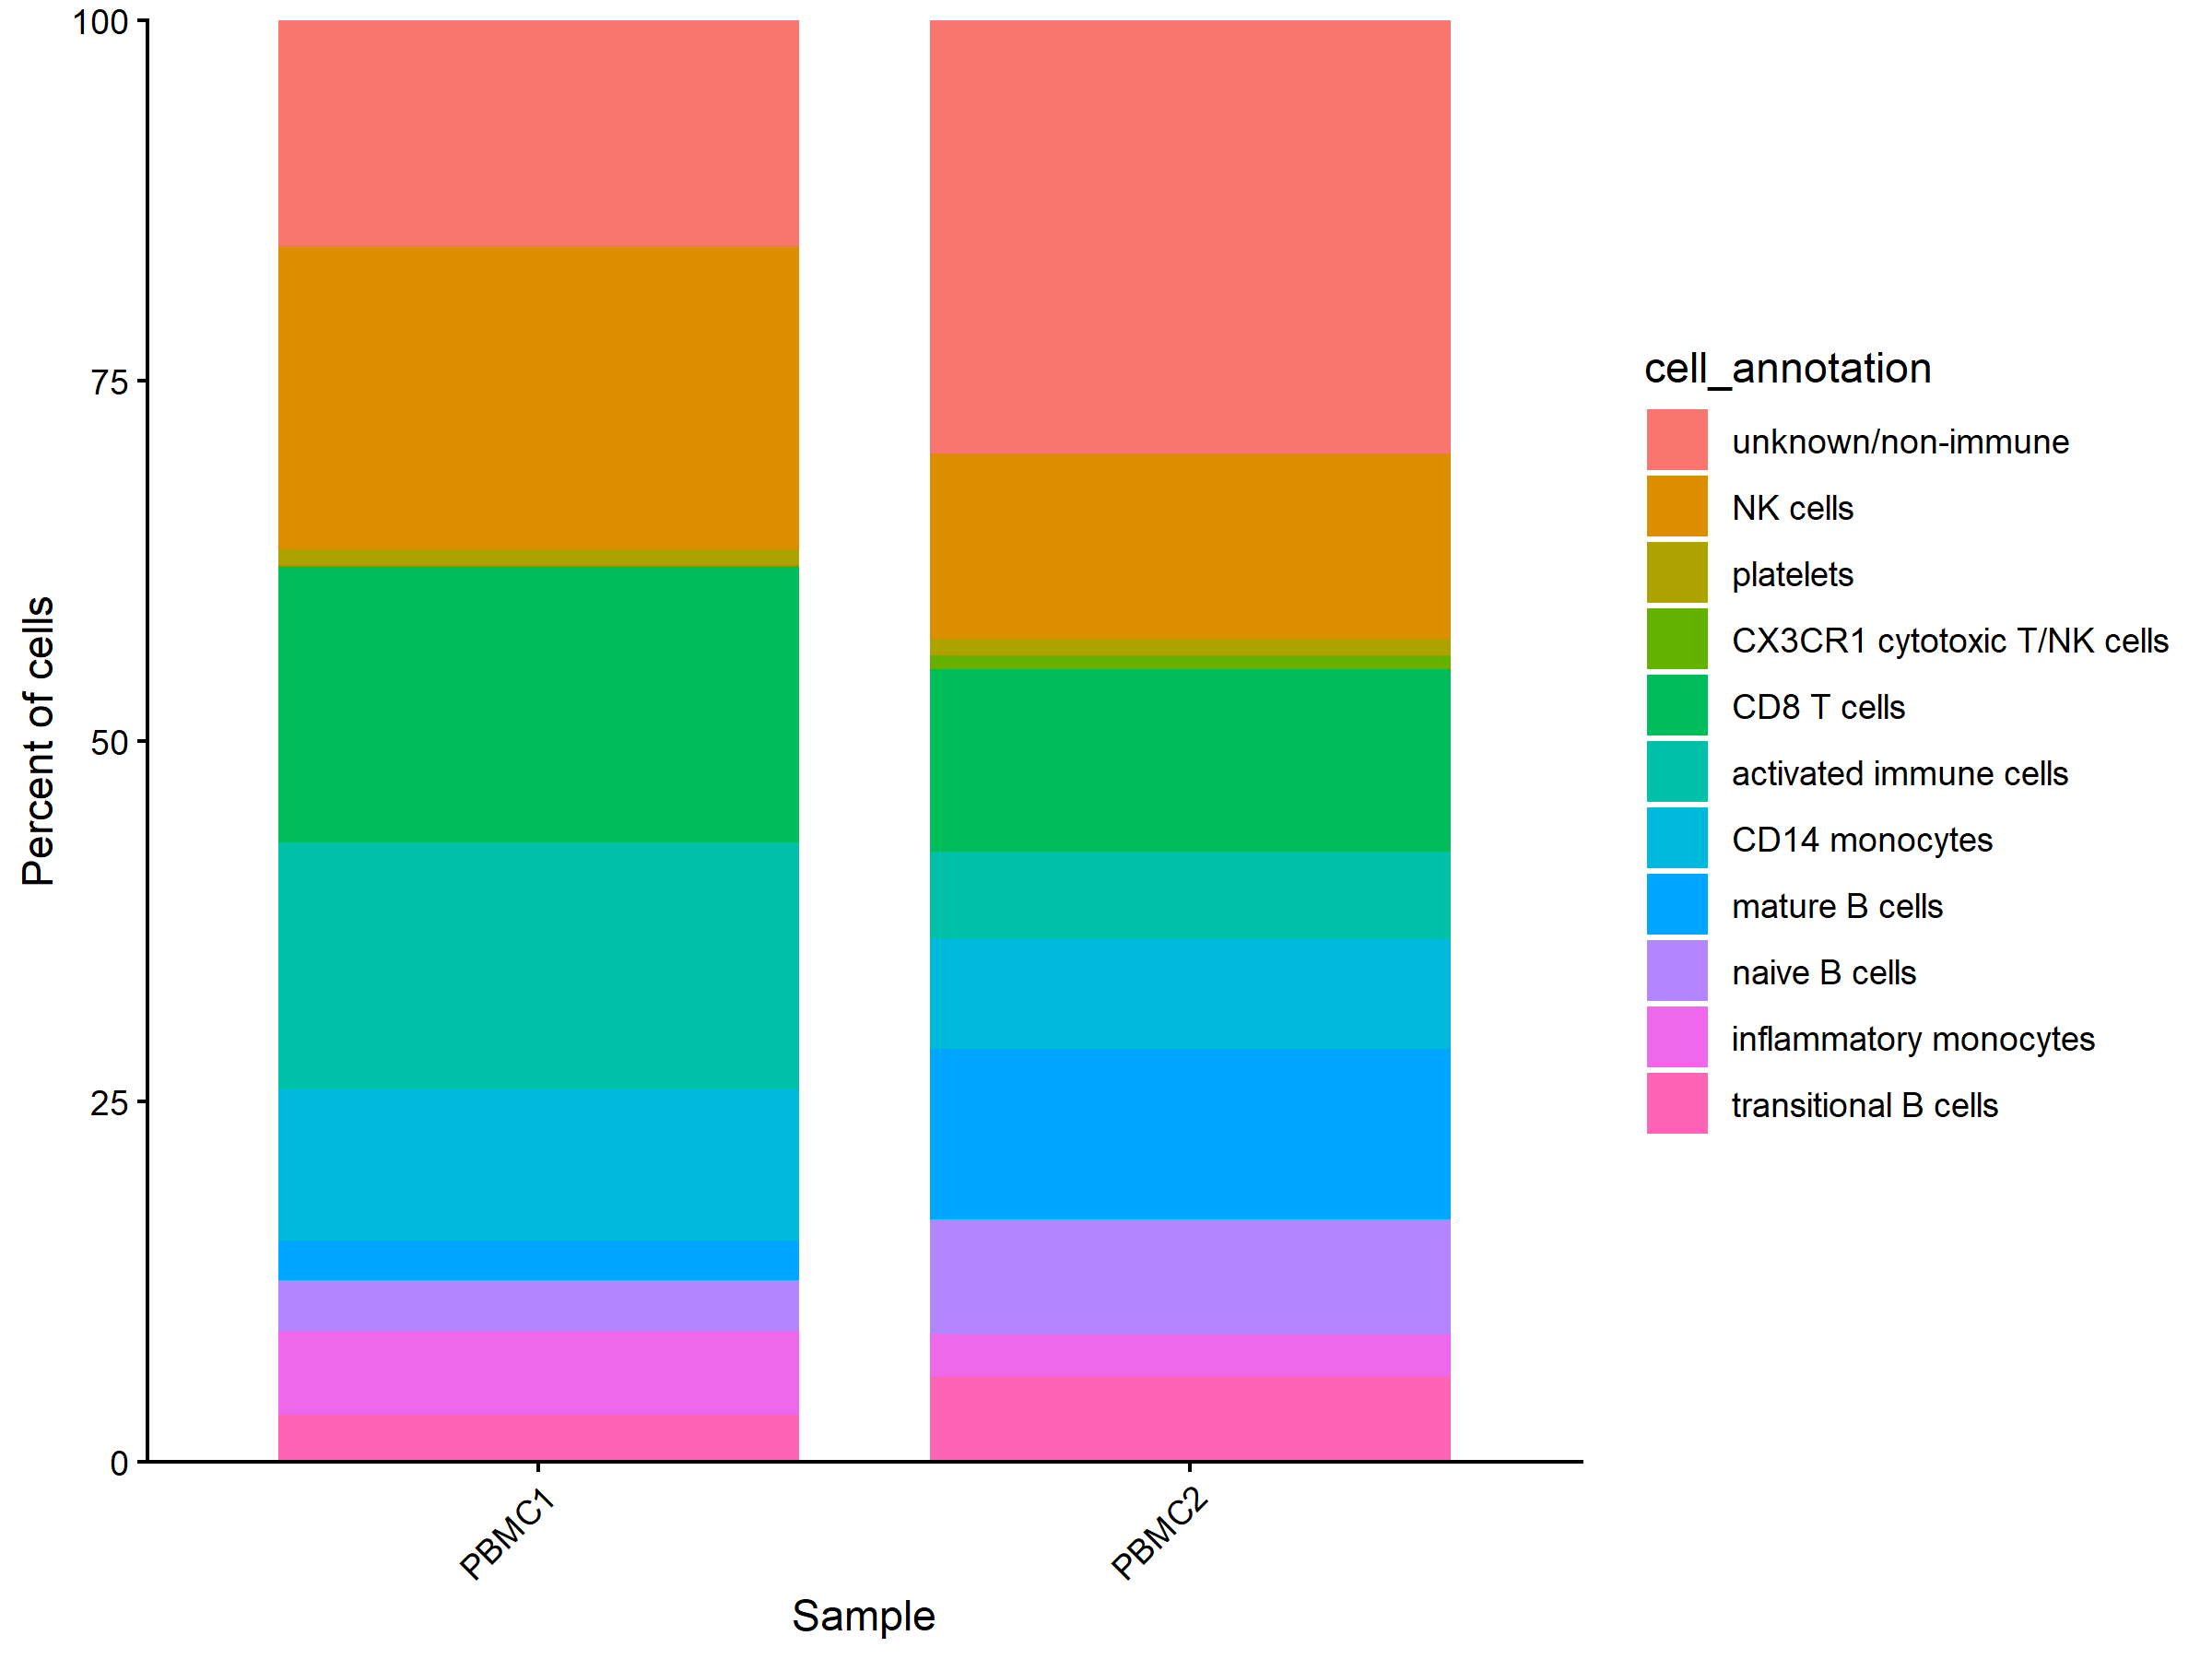
\includegraphics[width=\linewidth]{Figures/cluster_composition_plot.png}
  \caption{Composition}
\end{subfigure}
\caption{Cluster composition section. Left: controls set to group cells by \texttt{cell\_annotation} with one bar per sample. Right: the percent of cells in each of the 11 annotated cell types in samples PBMC1 and PBMC2.}
\label{fig:viz_composition}
\end{figure}
\FloatBarrier

\textbf{Output.}
Each section shows its plot in the app with a download button. The downloaded file uses the filename, format, and size set in that section. Plots are kept only for the current session (see \emph{Sessions and downloads} in the Overview).

\end{document}
